\documentclass{article}
\usepackage[utf8]{inputenc}
\usepackage{array}
\usepackage{multirow}
\usepackage{graphicx}
\usepackage{rotating}
\usepackage{color}   %May be necessary if you want to color links
\usepackage{hyperref}
\usepackage{longtable}
\usepackage{float}
\usepackage[table]{xcolor}
\usepackage{amssymb}
\usepackage{minted}
\setlength{\arrayrulewidth}{0.5mm}
\setlength{\tabcolsep}{18pt}
\renewcommand{\arraystretch}{2.5}
\hypersetup{
    colorlinks=false, %set true if you want colored links
    linktoc=all,     %set to all if you want both sections and subsections linked
    %linkcolor=blue,  %choose some color if you want links to stand out
}

\title{DREAM - RASD}
\author{Filippo Lazzati}
%\date{October 2021}

\begin{document}
\thispagestyle{empty} 
\begin{titlepage}
    \begin{center}
       %\vspace*{2cm}
       {\Huge \textbf{DREAM}} %%Replace this with the Title of your research
       \vspace{0.5cm}
       \\
    \begin{LARGE}
        {Data-dRiven PrEdictive FArMing in Telangana}
        \vspace{1.0cm}
        \\
        {\textit{Requirement Analysis and Specification Document - RASD}}
        
\includegraphics[width=13cm]{logo/polimi.png}
       \vspace{1.5cm}
        
        {Christian Grasso - Filippo Lazzati - Chiara Magri}
       \vspace{0.5cm}
       {Year: 2021/2022}
       
    \end{LARGE}  
   \end{center}
\end{titlepage}
\newpage
\tableofcontents 
\newpage
\listoffigures
\newpage
\listoftables
\newpage
\section{Introduction}
A RASD is a document that aims to present all the requirements of the system to be developed, explaining the 
domain in which it has to operate. A RASD should work as baseline for the following tasks in software development,
in particular in project planning, software evaluation and change control. Such document has a wide audience, and hence it has to
be written as clear as possible.
\subsection{Purpose}
The main goal that Telangana’s government wants to achieve with \verb|DREAM| is to help policy makers 
formulating policies in the field of agriculture. In order to accomplish this objective, Telangana’s 
government is asking for predictive models for food systems that can drive decisions exploiting huge 
amount of data. Therefore, \verb|DREAM| must be a software system that gathers data from some sensors and from the farmers and the agronomists and performs data analysis over it in order to help policy makers doing their job. Moreover, \verb|DREAM| aims to help farmers by putting them in contact with each other so that they can exchange advice and aids. Finally, \verb|DREAM| also schedules the daily work of agronomists and their visits to farmers.\\
Consequently, the goals of this project are:
\rowcolors{2}{gray!15}{gray!35}
 \begin{longtable}[c]{|m{0.75cm}|m{11cm}|}
  \caption{List of goals.}
 \label{Goals}
%%%%%%%%%%%%%%%%%%%%%%%%%%%%%%%%%%
 \hline
 \multicolumn{2}{|c|}{\cellcolor{white}\textbf{\emph{Goals}}}
 % do not write anything here
 \endfirsthead
 % do not write anything here
 \endhead
 % do not write anything here
 \endfoot
 % do not write anything here
 \endlastfoot
%%%%%%%%%%%%%%%%%%%%%%%%%%%%%%%%%
\hline
G1\label{G1} & The \verb|policy makers| are able to identify the best-performing farmers and the worst-performing farmers\footnote{See section \ref{Abbreviations}}.\\
  \hline
G2\label{G2} & The \verb|policy makers| are able to understand whether the initiatives involving agronomists and best-performing farmers have a good impact on the work of the farmers.\\
\hline
G3\label{G3} & \verb|Farmers| visualize weather forecasts regarding their piece of land.\\
  \hline
G4\label{G4} & The \verb|farmers| receive personalized suggestions about crops to plant and fertilizers to use.\\
  \hline
G5\label{G5} & The \verb|farmers| ask for and receive help from agronomists and other farmers.\\
  \hline
G6\label{G6} & The \verb|agronomists| can plan farm visits based on the farmers performances.\\
  \hline
  G7\label{G7} & The \verb|farmers| can interact with other farmers exchanging opinions about agriculture.\\
  \hline
  G8\label{G8} & The \verb|agronomists| visualize weather forecasts regarding the area they are responsible of.\\
  \hline
  G9\label{G9} & The \verb|agronomists| are able to identify the best-performing farmers and the worst-performing farmers\footnotemark[1] of the area they are responsible of.\\
  \hline
  \end{longtable}
\subsection{Scope}
\verb|DREAM| is a software system that has to work in a \textit{World}\footnote{The world is the portion of the real-world affected by the machine. See section \ref{Abbreviations}} where the following phenomena occur\footnote{Here World-only phenomena are listed, that is the World phenomena which are not shared with the Machine. If W is the set of World phenomena and M is the set of Machine phenomena, here elements of the (W - M) set are listed.}:
\rowcolors{2}{gray!15}{gray!35}
\begin{longtable}[c]{|m{0.75cm}|m{11cm}|}
 \caption{List of world phenomena.}
 \label{World phenomena}
 \hline
 \multicolumn{2}{|c|}{\cellcolor{white}\textbf{\emph{World phenomena}}}
 \hline
 % do not write anything here
 \endfirsthead
 % do not write anything here
 \endhead
 % do not write anything here
 \endfoot
 % do not write anything here
 \endlastfoot
 %%%%%%%%%%%%%%%%%%%%%%%%%%%%%%%% weather%%%%%%%%%%%%%%%%%%%%%%%%%%
 WP1\label{WP1} & In the mandal X, in the day YYYY/MM/DD, the \textbf{weather} is WW\footnote{WW is a label that, from now on, will be used to denote one of the following attributes: sunny, partially cloudy, cloudy, foggy, rainy, stormy, tornado, hurricane. See section \ref{Abbreviations}}.\\
 \hline
 WP2\label{WP2} & In the mandal X, the maximun, minimum and average \textbf{temperatures} in the day YYYY/MM/DD are TMAX, TMIN and TAVG.\\
 \hline
 WP3\label{WP3} & In the mandal X, the millimeters of \textbf{rain} fallen in the day YYYY/MM/DD are RR.\\
 \hline
 WP4\label{WP4} & In the mandal X, the average \textbf{wind} of the day YYYY/MM/DD has a speed of VV km/h and a direction DR\footnote{DR is a label that, from now on, will be used to denote one of the following directions: N, W, S, E, NW, NE, SE, SW. See section \ref{Abbreviations}}\\
 \hline
 WP5\label{WP5} & In the mandal X, the average \textbf{humidity} of the day YYYY/MM/DD  rate is HR.\\
 \hline
 WP6\label{WP6} & In the mandal X, the average atmospheric \textbf{pressure} of the day YYYY/MM/DD  rate is AP millibars.\\
 %%%%%%%%%%%%%%%%%%%%%%%%%%% soil sensors%%%%%%%%%%%%%%%%%%%%
 
 \hline
 WP7\label{WP7} & The soil moisture\footnote{The soil moisture is defined as the mass of water/mass of solid particles in the terrain – or volume, depending on the definition} on a terrain T is SM.\\
 \hline
 %%%%%%%%%%%%%%%%%%%%%%%%%% water irrigation system %%%%%%%%%%%%%%%%%%

 WP8\label{WP8} & The water irrigation system  of a terrain TT spreads a quantity WI of water during the day YYYY/MM/DD.\\
 \hline
 %%%%%%%%%%%%%%%%%%%%%%%%farmers %%%%%%%%%%%%%%%%%%%%%%%%%%%%%%%
 WP9\label{WP9} & A farmer works in a plot of land of area A (and/or lives in the corresponding farm) in the mandal X.\\
 \hline
 WP10\label{WP10} & A terrain of area A is cultivated with product P.\\
 \hline
 WP11\label{WP11} & A farmer during the day YYYY/MM/DD plants an area A of product PR.\\
 \hline
  WP12\label{WP11} & A farmer during the day YYYY/MM/DD seeds an area A of product PR.\\
 \hline
 WP13\label{WP12} & A farmer during the day YYYY/MM/DD harvests a quantity of K kgs of product PR.\\
 \hline
 WP14\label{WP13} & A farmer during the day YYYY/MM/DD uses a quantity FQ of fertilizer on a plant P.\\
 \hline
 WP15\label{WP14} & A farmer manually irrigates one of his fields.\\
 \hline
 WP16\label{WP15} & A farmer faces a problem during his work.\\
 \hline
 %%%%%%%%%%%%%%%%%%%%%%%%% policy makers 
 WP17\label{WP18} & A policy maker is given a password by the Telangana administration.\\
 \hline
 %%%%%%%%%%%%%%%%%%%%%%%% agronomists %%%%%%%%%%%%%%%%%%%%%%%%%%%%%
 
 WP18\label{WP20} & An agronomist is given a password by the Telangana administration.\\
 \hline
 WP19\label{WP21} & An agronomist visits a farm.\\
 \hline
  WP20\label{WP22} & An agronomist is responsible for an area A of terrains.\\
 \hline
 \end{longtable}
 \newpage
 The shared phenomena\footnote{Shared phenomena are the intersection between World phenomena W and Machine phenomena M: W\cap  M} are:
 \rowcolors{2}{gray!15}{gray!35}
 \begin{longtable}[c]{|m{0.75cm}|m{11cm}|}
  \caption{List of shared phenomena.}
 \label{Shared phenomena}
 \hline
 \multicolumn{2}{|c|}{\cellcolor{white}\textbf{\emph{Shared phenomena}}}
 % do not write anything here
 \endfirsthead
 % do not write anything here
 \endhead
 % do not write anything here
 \endfoot
 % do not write anything here
 \endlastfoot
  \hline
  %%%%%%%%%%%%%%%%%%%%%%%%%%%%%%%%% forecasts %%%%%%%%%%%%%%%%%%%%%%%%%%%%%%%%%%
 SP1\label{SP1} & The forecast indicates that in the mandal X, in the day YYYY/MM/DD, the weather will be WW.\\
 \hline
 SP2 & The forecast indicates that in the mandal X, in the day/week/month the maximun, minimum and average temperatures will be TMAX, TMIN and TAVG.\\
 \hline
 SP3 & The forecast indicates that in the mandal X, in  the day/week/month the millimeters of rain fallen will be RR.\\
 \hline
 SP4 & The forecast indicates that in the mandal X, in the day/week/month, the average wind will have a speed of VV km/h and a direction DR.\\
 \hline
 SP5 & The forecast indicates that in the mandal X, in the day/week/month, the average humidity  rate will be HR.\\
 \hline
 SP6 & The forecast indicates that in the mandal X, in the day/week/month, the average pressure will be AP millibars.\\
 \hline
 %%%%%%%%%%%%%%%%%%%%%%%%%%%%%%%% weather reports %%%%%%%%%%%%%%%%%%%%%%%%%%%%%%%%%%%%%

 SP7 & The weather reports indicate that in the mandal X, in the day YYYY/MM/DD,  the weather was WW.\\
 \hline
 SP8 & The weather reports indicate that in the mandal X, in  the day/week/month the maximun, minimum and average temperatures in the day YYYY/MM/DD were TMAX, TMIN and TAVG.\\
 \hline
 SP9 & The weather reports indicate that in the mandal X, in the day/week/month the millimeters of rain fallen were RR.\\
 \hline
 SP10 & The weather reports indicate that in the mandal X, in the day/week/month, the average wind had a speed of VV km/h and a direction DR.\\
 \hline
 SP11 & The weather reports indicate that in the mandal X, in  the day/week/month, the average humidity rate was HR.\\
 \hline
 SP12 & The weather reports indicate that in the mandal X, in the day/week/month, the average atmospheric pressure was AP millibars.\\
 \hline
 %%%%%%%%%%%%%%%%%%%%%%%soil sensors%%%%%%%%%%%%%%%%%%%%%%%%%%%%

 SP13 & The soil moisture sensor detects a soil moisture on a terrain T of SM\%.\\
 \hline
 %%%%%%%%%%%%%%%%%%%%%%%%%%water irrigation system%%%%%%%%%%%%%%%%%%%%%%%%%%%

  SP14 & The water irrigation system  sensor of a terrain TT measures that a quantity WI of water  has been spread during the day YYYY/MM/DD.\\
 \hline
 %%%%%%%%%%%%%%%%%%%%%%%%%%%% farmers%%%%%%%%%%%%%%%%%%%%%%%%%%%%%%%%%%%%%%%

  SP15 & A farmer creates an account.\\
 \hline
  SP16 & A farmer logs in.\\
 \hline
 SP17 & A farmer inserts in \verb|DREAM| his personal data (name, surname, contacts).\\
 \hline
 SP18 & A farmer inserts in \verb|DREAM| the location and the area of the plot of land that he owns/is responsible of.\\
 \hline
 SP19 & A farmer inserts in \verb|DREAM| that in his piece of land, an area A is devoted to the cultivation of product P.\\
 \hline
 SP20 & A farmer inserts in \verb|DREAM| that during the day YYYY/MM/DD  he has sowed an area A of product PR.\\
  \hline
 SP21 & A farmer inserts in \verb|DREAM| that during the day YYYY/MM/DD  he has planted an area A of product PR.\\
 \hline
 SP22 & A farmer inserts in \verb|DREAM| that during the day YYYY/MM/DD he has harvested a quantity of K kgs of product PR.\\
 \hline
 SP23 & A farmer inserts in \verb|DREAM| during the day YYYY/MM/DD  that he has used a quantity FQ of fertilizer on a plant P.\\
 \hline
 SP24 & A farmer inserts in \verb|DREAM| that that during the day YYYY/MM/DD he has manually irrigated a piece of land PL with a quantity of water WI.\\
 \hline
 SP25 & A farmer visualizes the weather forecasts relative to its farm's location.\\
 \hline
 SP26 & A farmer visualizes a suggestion regarding a crop to plant or a fertilizer to use in its land.\\
 \hline
 SP27 & A farmer inserts into \verb|DREAM| data regarding a problem he has or he faced.\\
 \hline
 SP28 & A farmer issues a request for a visit of an agronomist.\\
 \hline
 SP29 & A farmer issues a request for help to an agronomist.\\
 \hline
 SP30 & A farmer issues a request for help to another farmer.\\
 \hline
 SP31 & A farmer responds to a request for help received by another farmer.\\
 \hline
 SP32 & A farmer shares a post on the discussion forum.\\
 \hline
 SP33 & A farmer creates a new discussion thread on the forum.\\
 \hline
  SP34 & A farmer receives the notification of the visit of an agronomist.\\
 \hline
 %%%%%%%%%%%%%%%%%%%%%%%%%%%%% policy makers %%%%%%%%%%%%%%%%%%%%%%%%%%%%%

 SP35 & A policy maker logs in.\\
 \hline
 SP36 & \verb|DREAM| shows statistics regarding farmers (type of products, amount produced, fertilizers, watering, location…).\\
 \hline
 SP37 & \verb|DREAM| shows a list of the best-performing farmers.\\
 \hline
 SP38 & \verb|DREAM| shows a list of the worst-performing farmers.\\
 \hline
 SP39 & \verb|DREAM| shows correlations between agronomists and good farmers interventions and farmers statistics\\
 \hline
 SP40 &  A policy maker selects a farmer from a list of best performing farmers and saves it as well performing farmer .\\
 \hline
 SP41 & A policy maker selects a farmer from a list of worst performing farmers and saves it as badly performing farmer .\\
 \hline
  %%%%%%%%%%%%%%%%%%%%%%%%%%%%% agronomists %%%%%%%%%%%%%%%%%%%%%%%%%%%%%

 SP42 & An agronomists logs in in the \verb|DREAM| system.\\
 \hline
 SP43 & An agronomist inserts the area A of terrains he is responsible of into the \verb|DREAM| system.\\
 \hline
 SP44 & An agronomist receives a request for help from a farmer.\\
 \hline
 SP45 & An agronomist replies to a request for help from a farmer.\\
 \hline
 SP46 & An agronomist visualizes the weather forecast for the area he is responsible of.\\
 \hline
 SP47 & An agronomist visualizes a list of the best-performing farmers in the area he is responsible of.\\
 \hline
 SP48 & \verb|DREAM| computes a daily plan  for an agronomist to visit the farms he is responsible of.\\
 \hline
 SP49 & An agronomist updates his daily plan for visiting farms.\\
 \hline
 SP50 & At the end of a work day, an agronomist confirms the execution of his daily plan for visiting farms.\\
 \hline
 SP51 & At the end of a work day, an agronomist specifies a deviation for his daily plan for visiting farms.\\
 \hline
 SP52 & An agronomist inserts into the system information regarding a visit to a farm.\\
 \hline
 SP53 & An agronomist visualizes data about a farmer he has to visit: the type of plants he grows, the seeded or planted quantities and the harvested quantities for each cultivation starting from the agronomist's last visit to the farmer and the problems inserted by the farmer since the last visit of the agronomist.\\
 \hline
 \end{longtable}

\subsection{Definitions, Acronyms, Abbreviations}\label{Abbreviations}
\begin{itemize}
    \item WW = sunny | partially cloudy |  cloudy | foggy  |  rainy | stormy | tornado | hurricane
    \item DR = North | West | South | East | North-West | North-East | South-East | South-West 
    \item farmer = citizen of Telangana who works on a piece of land
    \item agronomist = expert of agriculture in Telangana
    \item policy-maker = devises policies to regulate the agricultural
production of Telangana
    \item best/worst -performing farmer = farmer chosen by a policy-maker (or an agronomist) taking into account its performances
    \item world\footnote{{Michael Jackson. 1995. The world and the machine. In Proceedings of the 17th international conference on Software engineering (ICSE '95) Association for
Computing Machinery, New York, NY, USA, 283–292.
DOI:https://doi.org/10.1145/225014.225041}} = portion of the real-world
affected by the machine.
\item TSDPS = Telangana State Development Planning Society
\item machine = the portion of system to be developed.
\item weather report = historical meteorological data (so, referred to the past)
\item weather forecast= predicted meteorological data (so, referred to the future)
\end{itemize}
\subsection{Revision history}
\begin{left}
\begin{tabular}{ |c | c |}
\hline
 revision & changes \\ 
 \hline
 1.0 &  initial version\\ 
 \hline
\end{tabular}
\end{left}
\subsection{Reference Documents}
\begin{itemize}
\item \textit{IEEE 29148-2018 Requirements engineering}, the IEEE specification document that “provides details for the construct of well-formed textual requirements, to include characteristics and attributes, in the context of system and software engineering”;
\item course slides;
\item assignment document.
\end{itemize}
\subsection{Document Structure}
This document complies with the SRS\footnote{Software Requirements Specification} standard structure as it is defined in the \textit{IEEE 29148-2018 Requirements engineering}, section 9.6. Nevertheless, the order of the contents has been slightly changed in order to facilitate the readers in the reading of this specific RASD\footnote{Requirements Analysis and Specification Document} and an additional section about Alloy\footnote{\url{https://alloytools.org/}.} formal analysis has been added.
Therefore, the document is divided in 4 main parts:
\begin{enumerate}
\item the first part (to which this section belongs) provides an introduction to the system to-be, \verb|DREAM|, making clear which are the goals it is required to achieve and in which context it is going to operate;
\item the second part provides a more detailed description of the functions that \verb|DREAM| has to implement relating them to the main concepts of the system and to the user needs; it also provides the main assumptions under which \verb|DREAM| will work properly;

\item the third part contains the out-and-out requirements of the system, from both the functional and the non-functional points of view;
\item the fourth and last part contains a detailed analysis using a first order logic language (Alloy) of the trickiest requirements of the system.
\end{enumerate}
It should be remarked that the structure of this document does not follow a logic or temporal order, but whoever is interested in the reading can jump from a section to another, because the purpose of it is to be a reference document.
\newpage
\section{Overall description}
\subsection{Product perspective}
The requirements-level class diagram of \verb|DREAM| is:

\begin{sidewaysfigure}
    \centering
    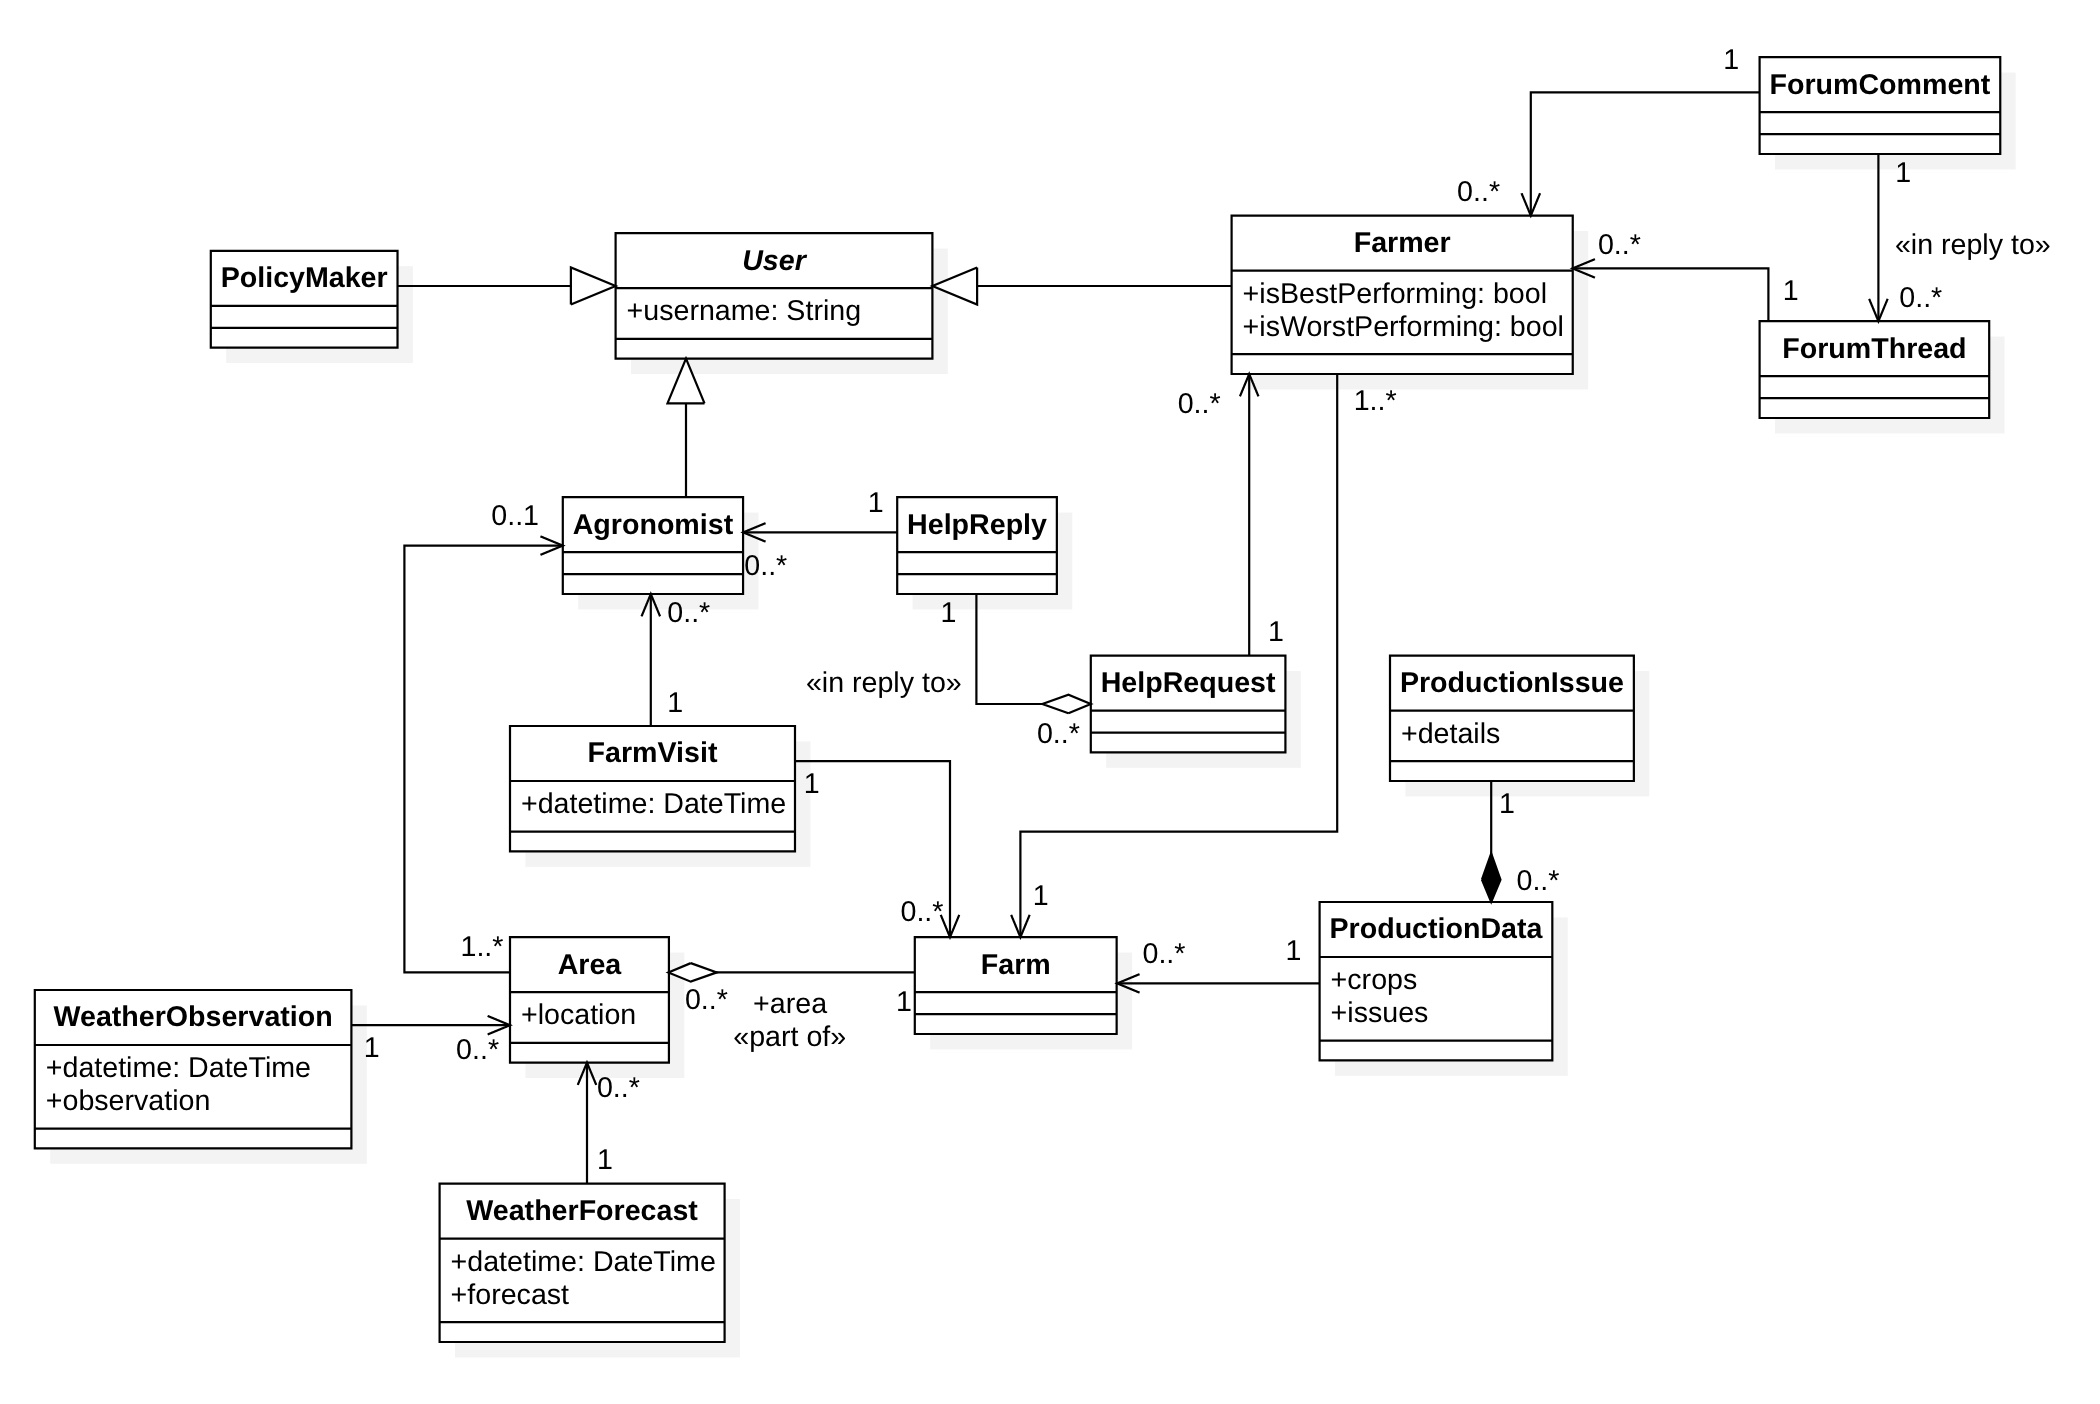
\includegraphics[scale=0.2]{class_diagrams/requirements-level class diagram.png}
    \caption{Requirements-level class diagram of DREAM.}
\end{sidewaysfigure}
\clearpage

The activity diagram for the creation of a new help request is:
\begin{figure}[H]
    \centering
	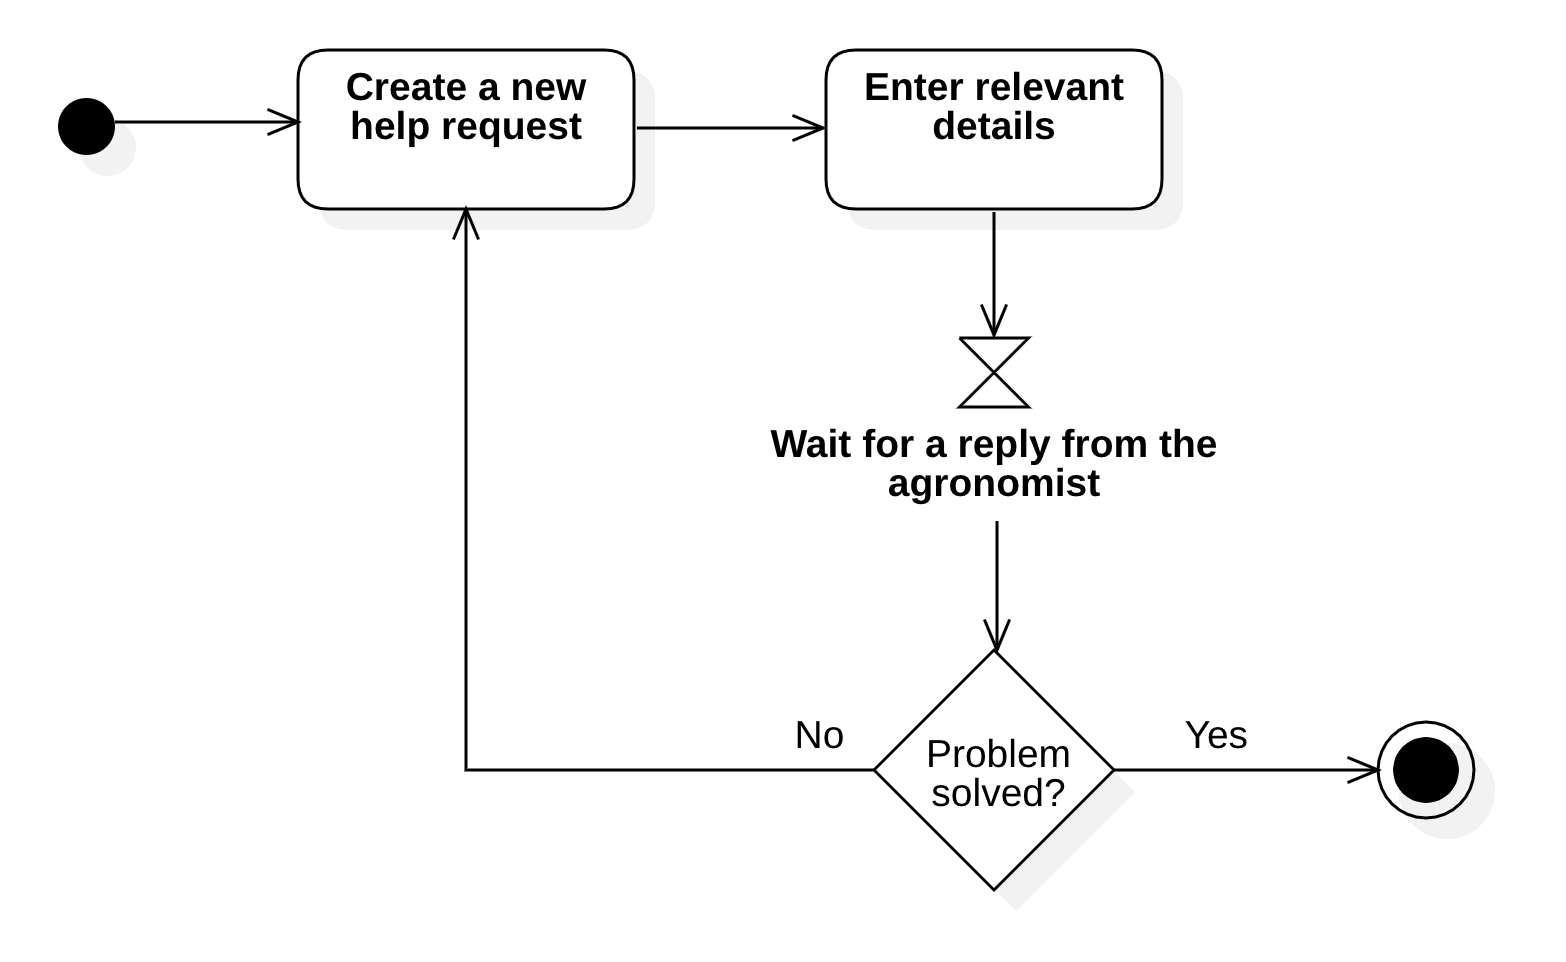
\includegraphics[scale=0.35]{state_machine_diagrams/statediagram1.png}
    \caption{Activity diagram for the creation of a new help request.}
\end{figure}

The activity diagram for the generation of a new daily plan is:
\begin{figure}[H]
    \centering
	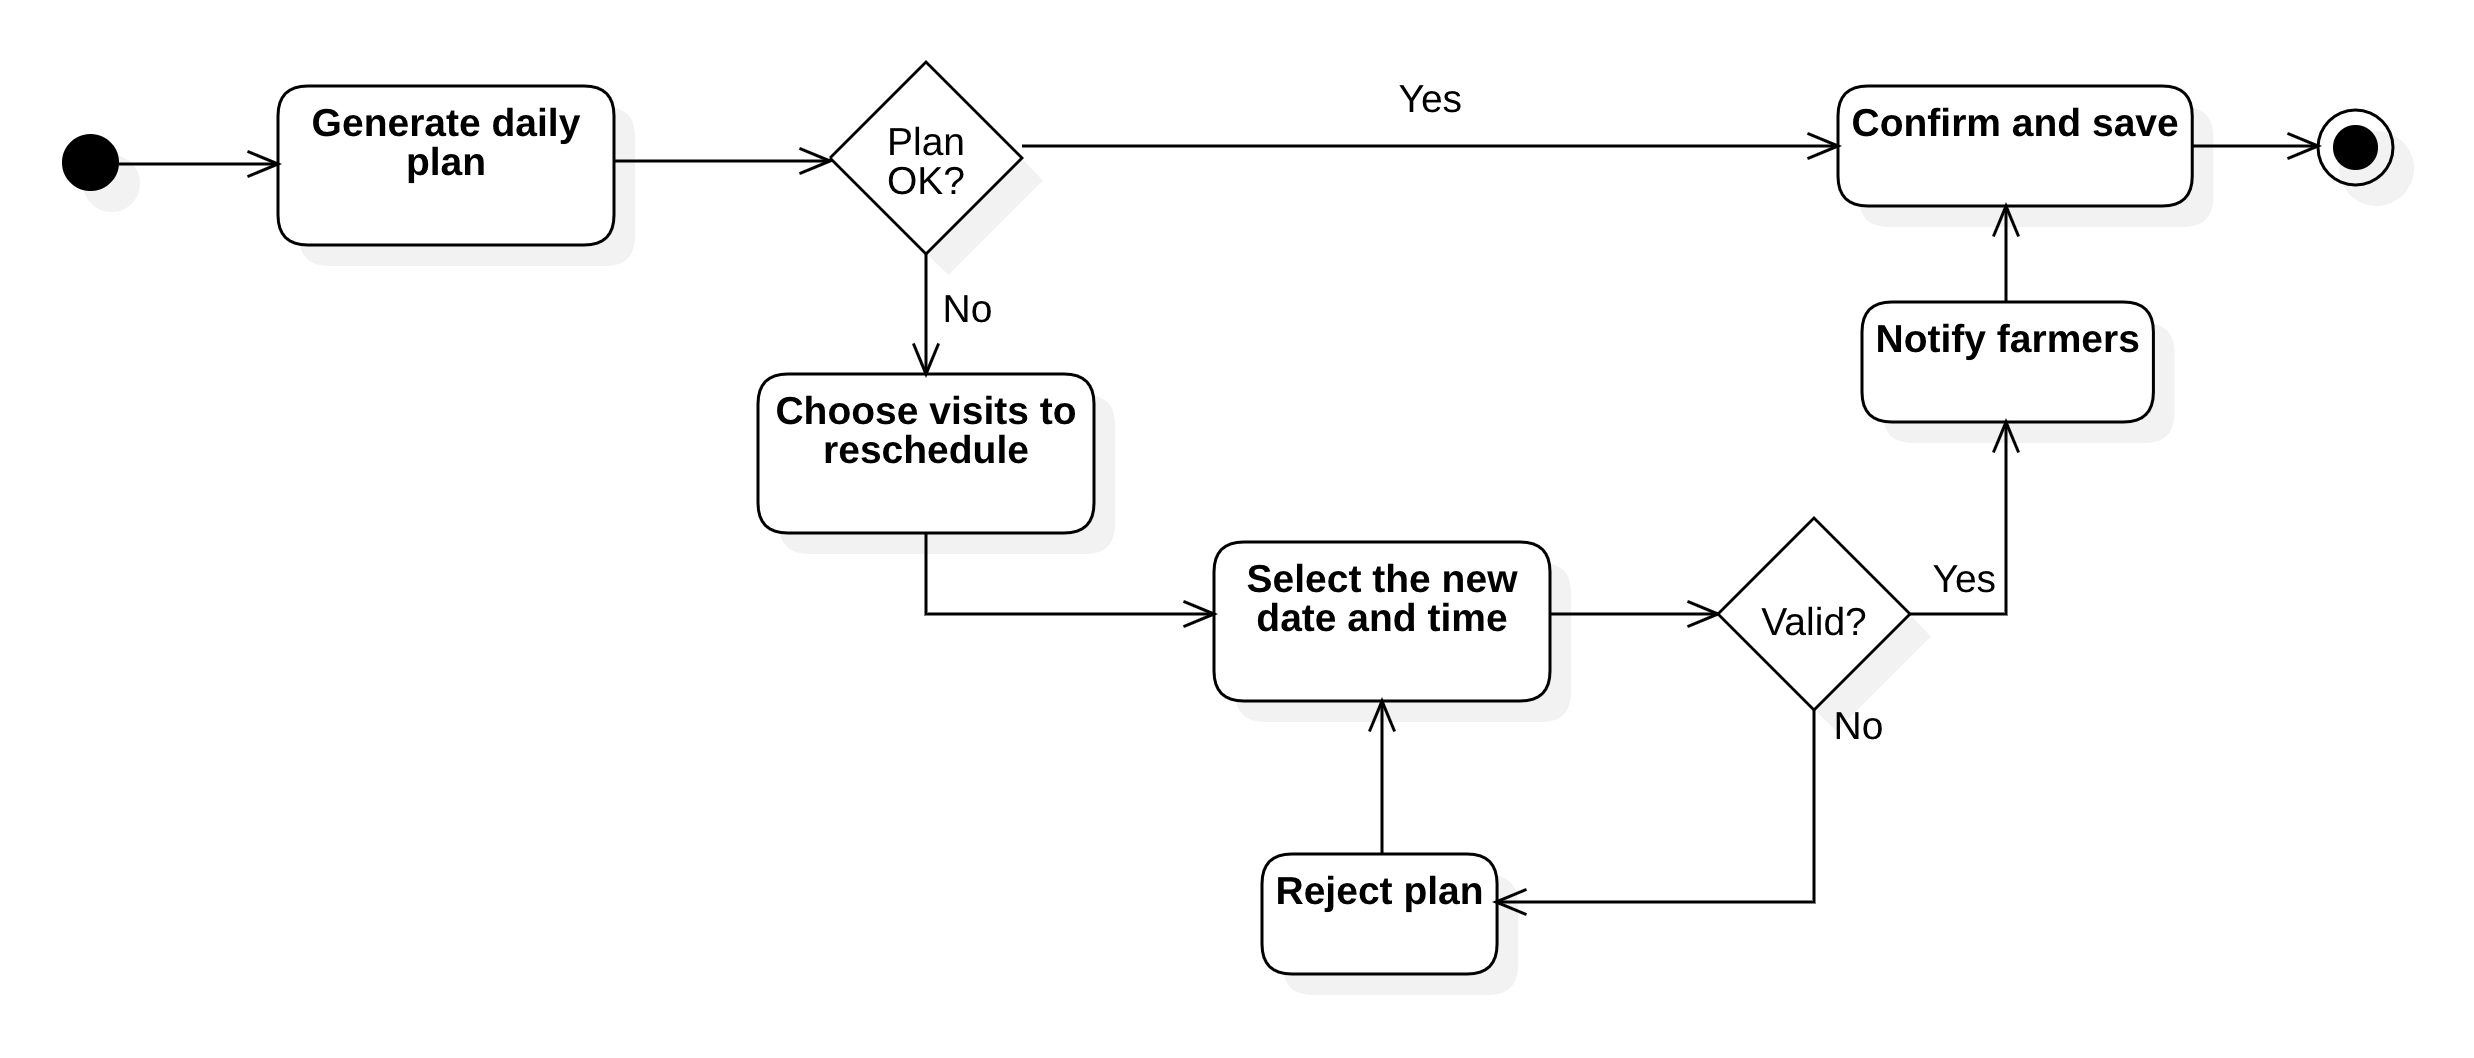
\includegraphics[scale=0.35]{state_machine_diagrams/statediagram2.png}
    \caption{Activity diagram for the generation of a new daily plan.}
\end{figure}
The activity diagram for the creation of a new production report is:
\begin{figure}[H]
    \centering
	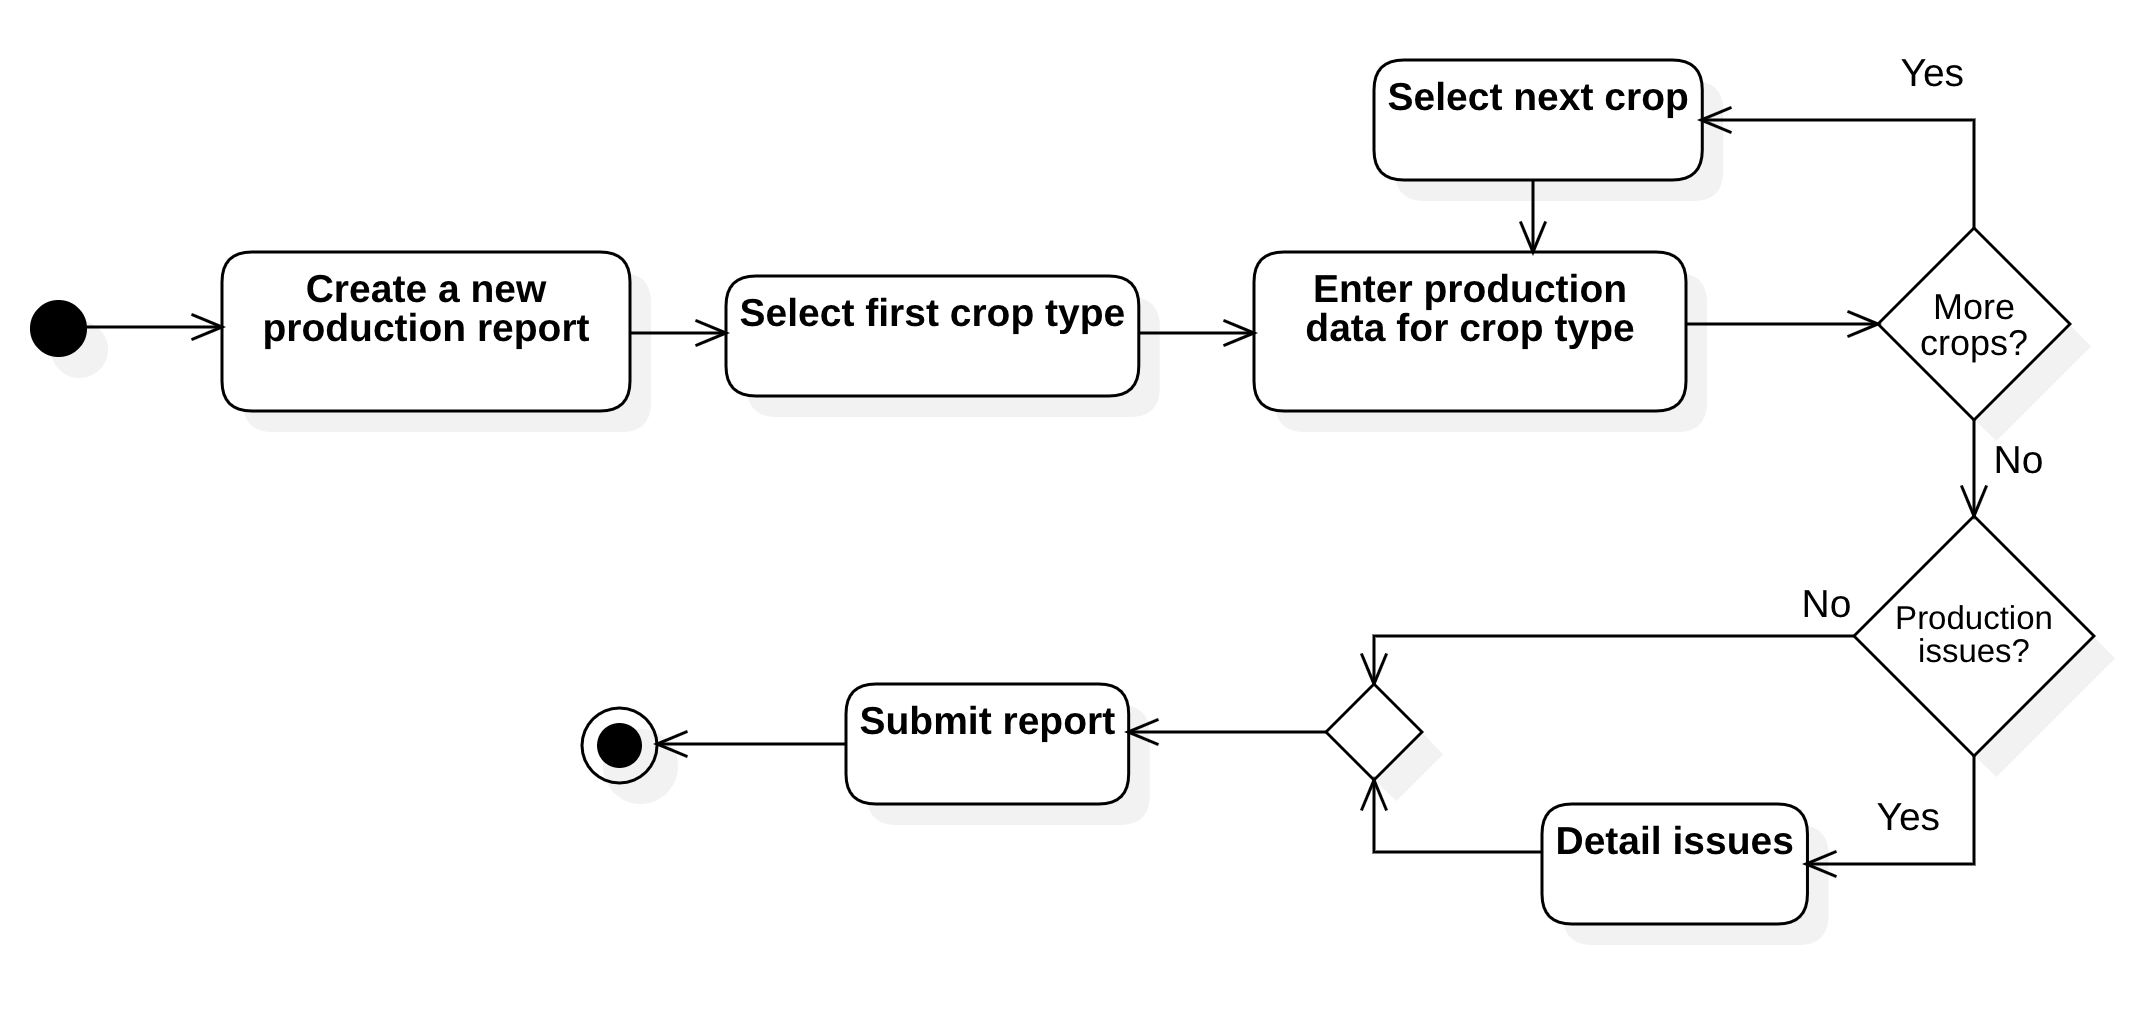
\includegraphics[scale=0.35]{state_machine_diagrams/statediagram3.png}
    \caption{Activity diagram for the creation of a new production report.}
\end{figure}
\subsection{Product functions} \label{Product functions}
In this section, a list of the most important requirements of the system is provided; notice 
that they are just briefly described, since they will be analysed in-depth in chapter 3.
\subsubsection{Data collection}
\verb |DREAM| must be able to manage different kinds of data coming from different sources:
\begin{enumerate}
\item agronomists and farmers insert into the system standard kind of information about the farms they 
respectively visit and own, but also other kinds of information like, for example, the types of products 
cultivated and the production volume for each product (kinds of information that allow the analytics to 
profile these users). \verb |DREAM| also allows them to insert less-structured data, for instance full-text feedback 
about the inserted data (farmers can insert data about any problem they face);
\item data gathered by sensors deployed on the territory and by the water irrigation system are automatically 
collected by \verb|DREAM| through effective interfaces interacting with such systems;
\item already existing systems are integrated with \verb|DREAM|;
\item the last but not the least, farmers can interact through discussion forums, that are stored by \verb|DREAM|.
\end{enumerate}
\subsubsection{Data analysis}
The raw data collected by \verb|DREAM| must be processed before being delivered to the end-user. Therefore, 
starting with the big volume of information “ingested”, various kinds of analytics are performed in order to 
provide a more aggregate version of the data:
\begin{itemize}
%machine learning techniques are used to customize (for example) the suggestions recommended to the 
%farmers based on their location and their type of production;
\item the suggestions provided to the farmers are customized according to their information;
\item information about farmers’ production is used to distinguish among farmers who are performing well 
and those who are not;% (classification problem);
%data mining algorithms are used to track patterns and identify relations
\item  patterns and relations are identified among the data (for instance between weather 
forecasts and production volumes);
% statistical algorithms are applied for quantifying the improvement (if present) in the crop after having 
% adopted agronomists’ suggestions.
\item analytics are also used for quantifying the improvement (if present) in the crop after having adopted agronomists’ suggestions.
\end{itemize}
\subsubsection{Forum}
As previously mentioned, farmers are allowed to open discussion forums on \verb|DREAM| with other farmers. 
This allows to keep in touch with other people doing the same job and, hence, to ask for advice in case of 
needing.
\subsubsection{Request and supply of help}
There are four different ways for a farmer to ask for help: ask for it directly to other farmers, ask in the forum, ask to
the agronomists or ask for a visit of an agronomist. It should be remarked that a farmer can contact only 
agronomists in the same area.
\subsubsection{Daily plan}
\verb|DREAM| automatically devises a daily plan for each agronomist consisting in a list of farms that must be visited and provides a possible time schedule for such meetings. Every daily plan must be actively accepted 
by the agronomist before the involved farmer is notified. Anyway, the agronomist can apply some changes 
to the schedule, but the system will not approve them if some constraints are violated.
\subsection{User characteristics}
With regards to the possible actors of \verb|DREAM|, three different main user classes can be identified:
\begin{description}
\item \textbf{Policy makers}: their job is to devise policies to regulate the agricultural production. \verb|DREAM| helps 
them providing aggregate data. Policy makers access the system and then receive high-level 
information about which farmers are performing well and which not, and possible reasons to this 
fact. Furthermore, \verb|DREAM| helps to understand the impact of agronomists’ clues in farmers’ 
productions;
\item \textbf{Farmers}: they have a farm and some plots of land to cultivate. They access the system and insert 
data about themselves, helping \verb|DREAM| to profile them. They insert data about their productions, 
the area where they work, eventual problems they must face, questions in the forum … and so on. 
On the other side, \verb|DREAM| puts them in touch with someone who can help them and provides data 
that may be relevant to them;
\item \textbf{Agronomists}: an agronomist has to find methods for increasing the production and the quality of 
the harvest. They insert the area they are responsible of and the they receive data about the best 
performing farmers and weather forecasts. They can answer to farmers’ questions and they receive 
a daily plan about which farmers they should visit.
\end{description}
\subsection{Assumptions, dependencies and constraints}

\rowcolors{2}{gray!15}{gray!35}
\begin{longtable}[c]{|m{0.75cm}|m{11cm}|}
 \caption{List of domain assumptions.}
 \label{Domain assumptions}
%%%%%%%%%%%%%%%%%%%%%%%%%%%%%%%%%%
 \hline
 \multicolumn{2}{|c|}{\cellcolor{white}\textbf{\emph{Domain assumptions}}}
 % do not write anything here
 \endfirsthead
 % do not write anything here
 \endhead
 % do not write anything here
 \endfoot
 % do not write anything here
 \endlastfoot
%%%%%%%%%%%%%%%%%%%%%%%%%%%%%%%%%
  \hline
  D1 & The location of the sensors is known to the \verb|DREAM| system.\\
  \hline
   D2 & The location of the water irrigation systems is known to the \verb|DREAM| system.\\
  \hline
  D3 & The TSDPS provides weather forecasts and reports which can be accessed by \verb|DREAM|.\\
  \hline
  D4 & The weather reports provide sufficiently accurate data.\\
  \hline
  D5 & The water irrigation system provides data with a sufficiently accurate precision.\\
  \hline
  D6 & Soil moisture sensors provide data with a sufficiently accurate precision.\\
  \hline
  D7 & Each farmer owns at least one device connected to Internet.\\
  \hline
  D8 & Each farmer has the competences for properly accessing the \verb|DREAM| system and registering to it.\\
  \hline
  D9 & All the data the farmers insert is correct.\\
  \hline
  D10 & (Best-performing) farmers answer to help requests sent to them.\\
  \hline
  D11 & When a farmer does something to a certain area (for example, applies a fertilizer or harvests), he covers the whole area.\\
  \hline
  D12 & Each policy maker owns a personal computer, connected to the Internet network and with a browser installed.\\
 \hline
  D13 & Each policy maker has the competences for properly accessing the \verb|DREAM| system and using it.\\
  \hline
  D14 & Every policy maker is given a password – associated to his e-mail – by the Telangana agriculture department, and such account is known to \verb|DREAM|.\\
  \hline
  D15 & Each agronomist owns a device connected to the Internet network and with a browser installed.\\
  \hline
  D16 & The agronomists are given a password – associated to their mail – by the Telangana agriculture department and such account is known to \verb|DREAM|.\\
  \hline
  D17 & Each agronomist has the competences for properly accessing the \verb|DREAM| system and using it.\\
  
   \hline
  D18 & All the data the agronomists insert is correct.\\
  \hline
  D19 & Agronomists reply to help requests issued by farmers.\\
  \hline
  \end{longtable}
  \newpage
\section{Specific requirements}
\subsection{External Interface Requirements}
\subsubsection{User interfaces}
\verb|DREAM| is provided to the users, namely farmers, agronomists and policy makers, as a webapp, accessible through a browser on the web. Therefore, \verb|DREAM| is not given with a CLI\footnote{Command Line Interface} but only with a GUI\footnote{Graphical User Interface}. The rest of this subsection contains some wireframes that show an example of suitable user interface for \verb|DREAM|\footnote{According to the “IEEE 29148-2018 Requirements engineering” document, section 9.6.4.2, “A style guide for the user interface can provide consistent rules for organization, coding and interaction of the user with the system”.}.
\begin{figure}[H]
    \centering
    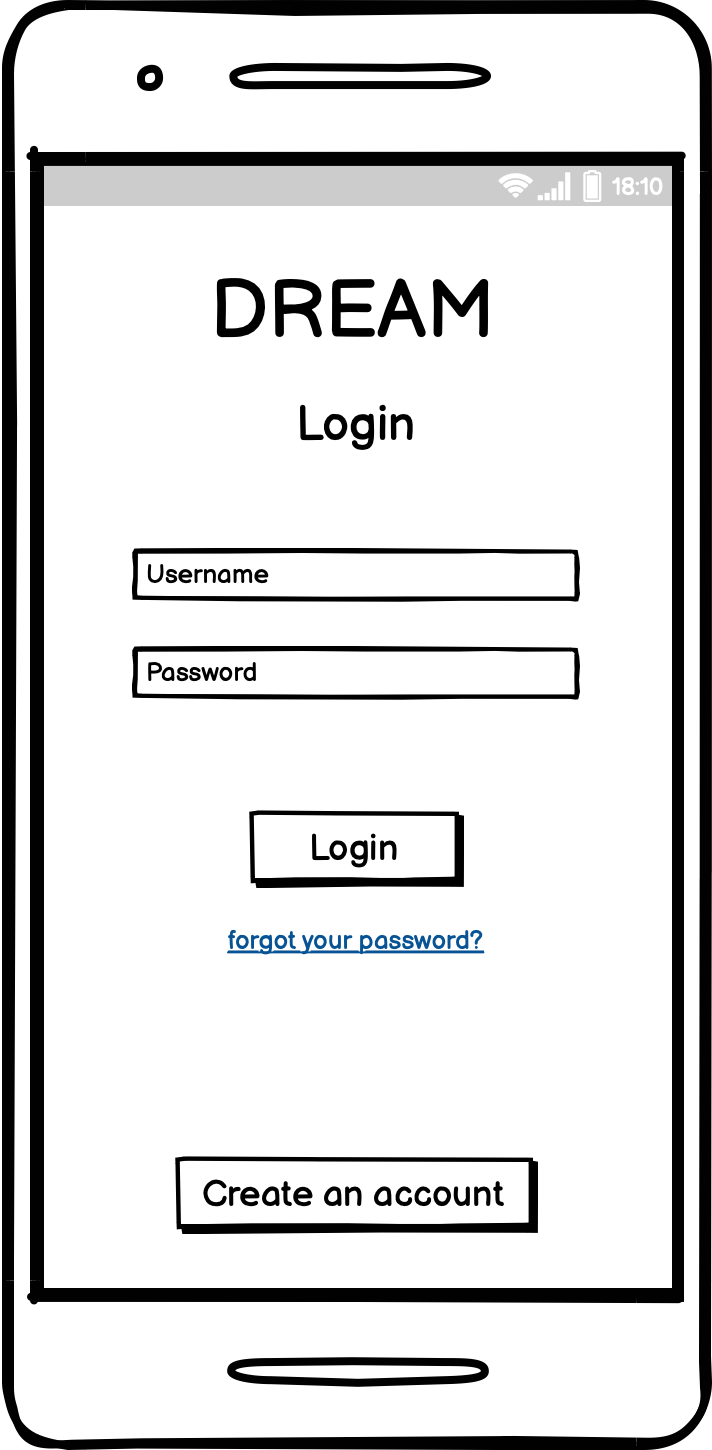
\includegraphics[scale=0.15]{wireframes/login.png}
    \caption{Wireframe of the initial page of the system.}
\end{figure}
\begin{figure}[H]
    \centering
    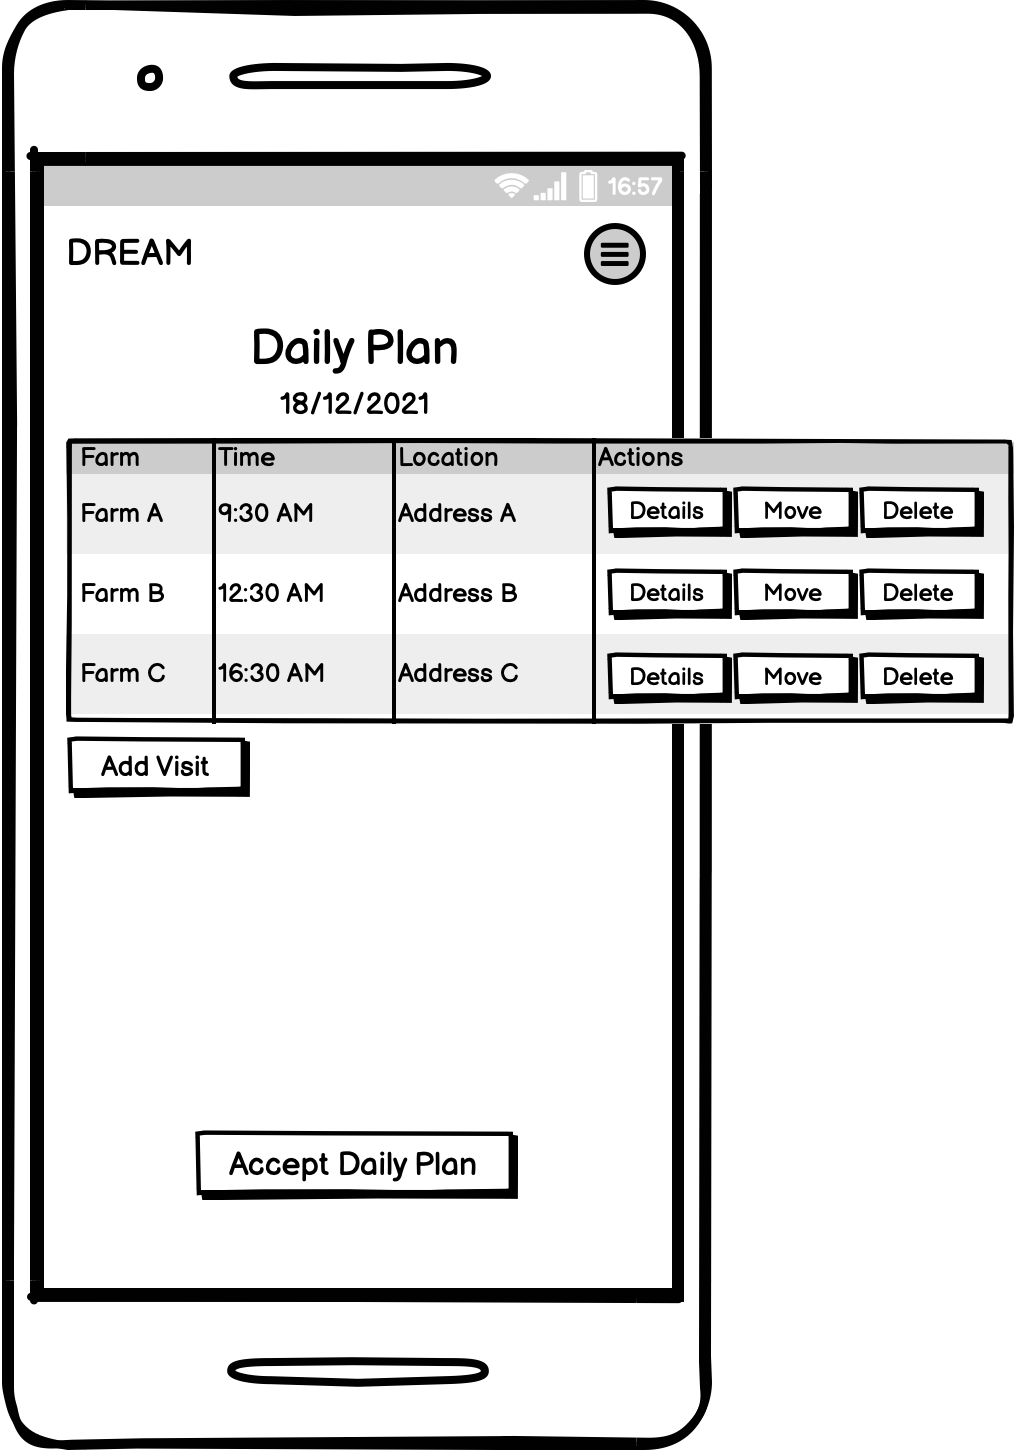
\includegraphics[scale=0.15]{wireframes/dailyplan.png}
    \caption{Wireframe of the page that allows to manage the daily plan.}
\end{figure}
\begin{figure}[H]
    \centering
    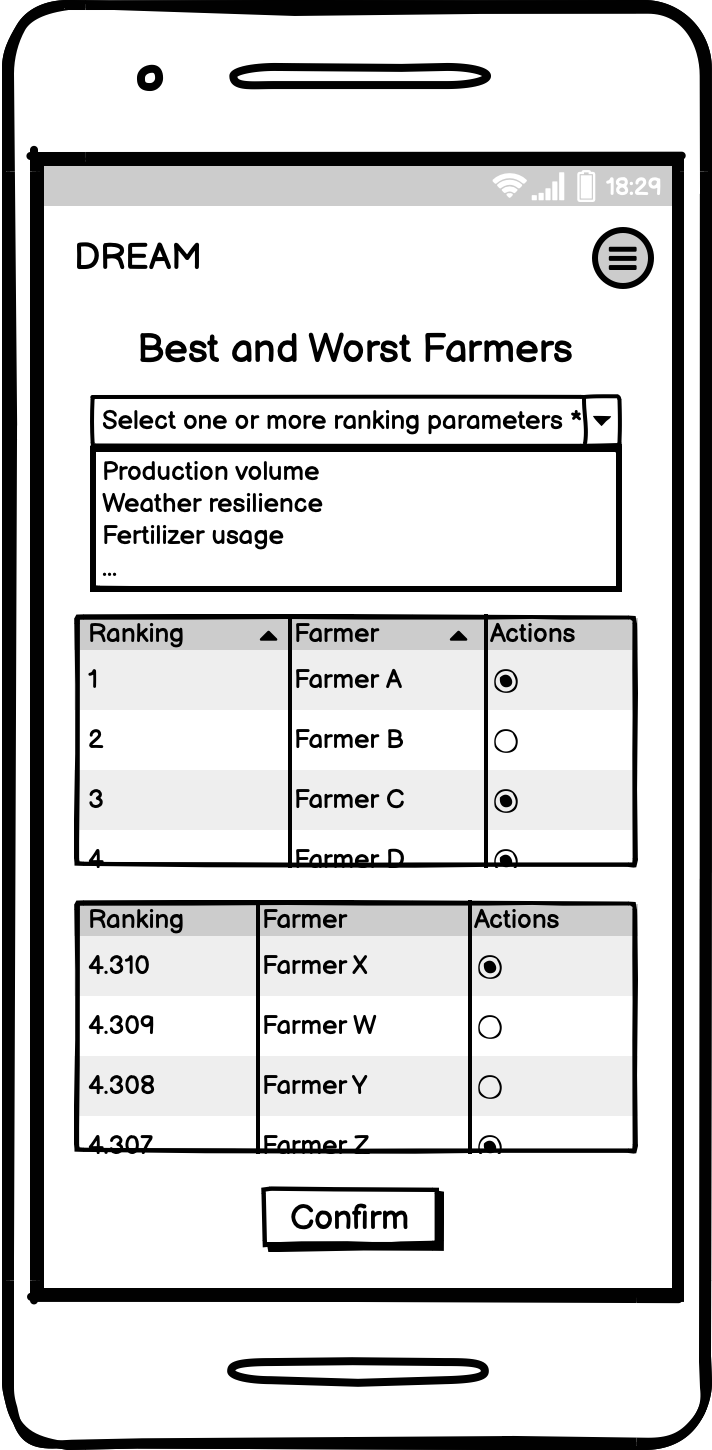
\includegraphics[scale=0.15]{wireframes/bestworstfarmers.png}
    \caption{Wireframe of the page that allows to rank the farmers.}
\end{figure}
\begin{figure}[H]
    \centering
    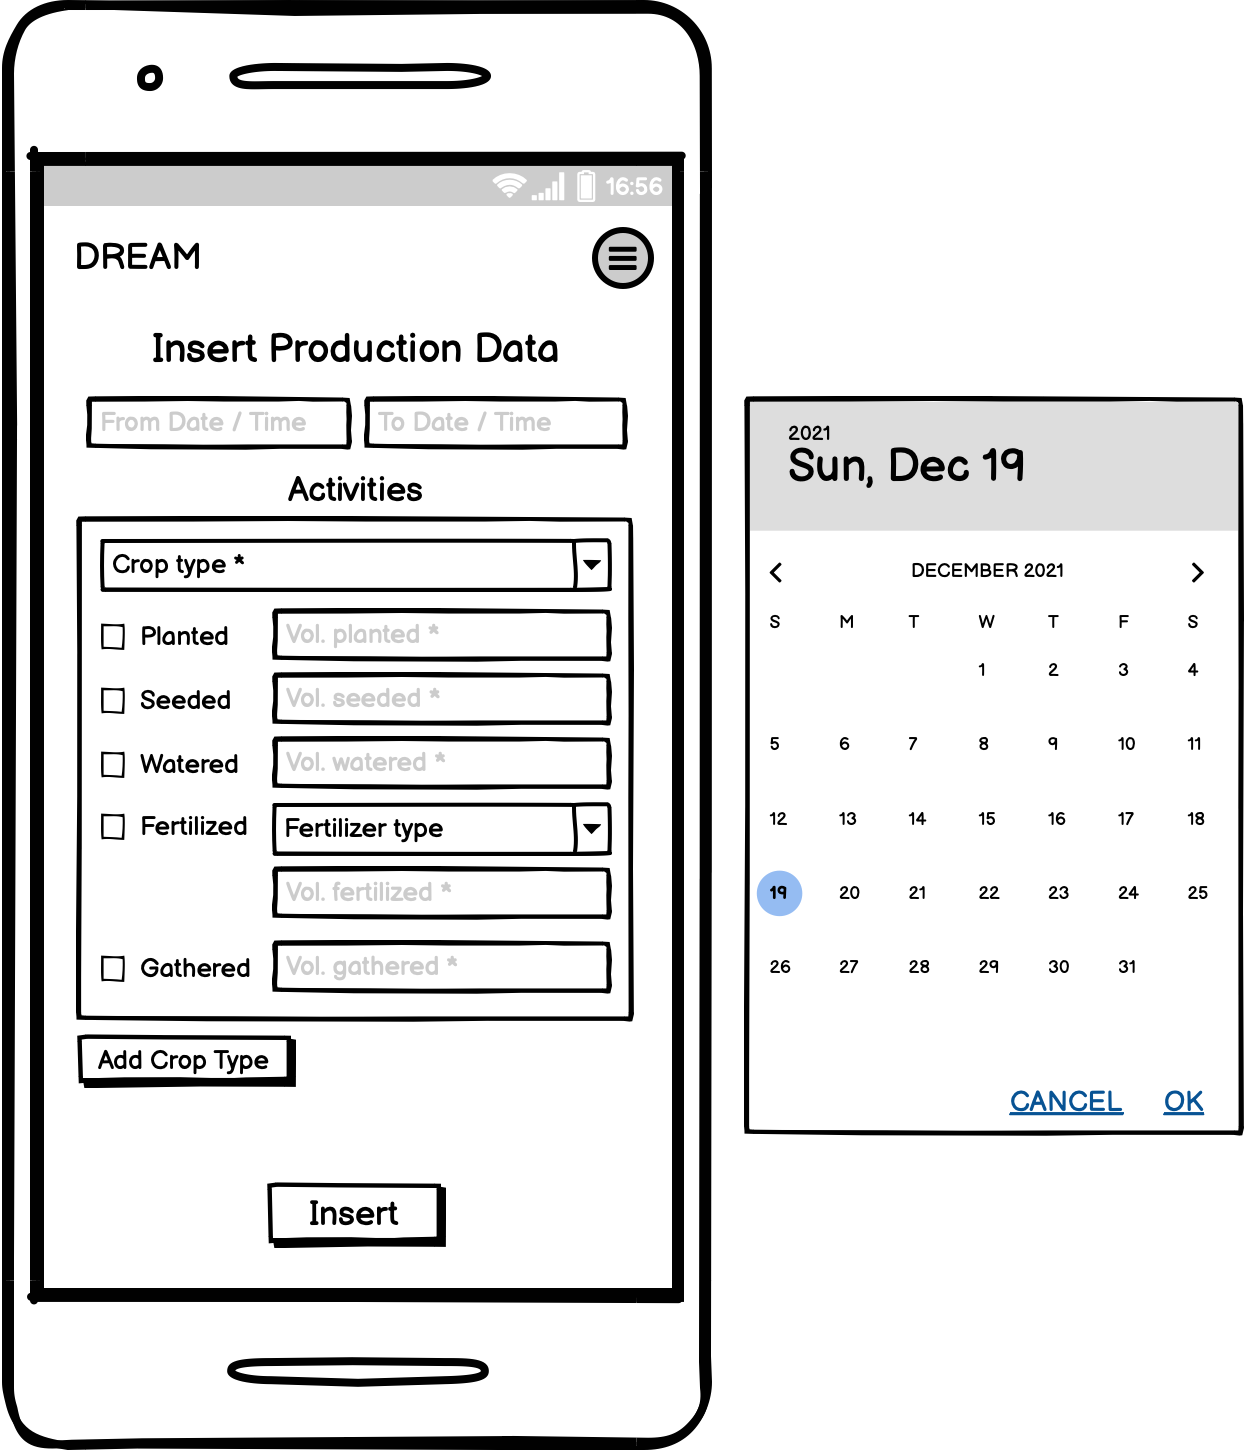
\includegraphics[scale=0.15]{wireframes/productiondata.png}
    \caption{Wireframe of the page that allows the insertion of production data.}
\end{figure}
\subsubsection{Hardware interfaces}
\begin{itemize}
\item Because \verb|DREAM| is to be implemented as a webapp, every user can access it through the device he prefers, that is personal computers, smartphones, tablets … and there is no requirement on the size of the device since the webapp has to be responsive (scale properly to different devices’ sizes). Every device of this kind suffices to achieve the goals.
\item \verb|DREAM| has to interact with various hardware components to gather the data it will use. In particular, \verb|DREAM| has to interact with soil sensors and a water irrigation system. Both these two systems are able to gather data and share it through a third already existing system (an IoT hub), to which they are connected through cables.
\end{itemize}
\subsubsection{Software interfaces}
The following software interfaces are required to make \verb|DREAM| work properly:
\begin{enumerate}
\item every user’s device must have a browser installed on it through which the user can access the \verb|DREAM|’s website; no other software requirements are requested to these kind of devices;
\item \verb|DREAM| requires the APIs to the Telangana’s government website\footnote{\url{https://www.tsdps.telangana.gov.in/aws.jsp}.} in order to retrieve weather reports and meteorological short-term and long-term forecasts;
\item \verb|DREAM| requires also an interface to the system that provides access to the data gathered by soil sensors and by the water irrigation system.
\end{enumerate}
\subsubsection{Communication interfaces}
As far as the communication interfaces are concerned, \verb|DREAM| uses:
\begin{enumerate}
    \item the HTTP protocol at the application layer (layer 7 of the stack) to exchange information (web pages) with the clients (users’ devices) and to access the data offered by the Telangana’s government systems;
    \item specific protocols for the communication to the sensor hub.
\end{enumerate}

\subsection{Functional Requirements}
\verb |DREAM| allows its users to perform many tasks, and \verb |DREAM| itself is able to interact with other different systems to achieve some results (see section \ref{Product functions}). In order to provide the main requirements of the system and a summary of the possible situations in which \verb |DREAM| is involved and used, this paragraph first lists all the requirements of the system, then it lists some concrete scenarios \footnote{“A narrative description of what people do and experience as
they try to make use of computer systems and applications” [M.
Carrol, Scenario-based Design, Wiley, 1995]} and finally it abstracts from details and specificities showing the corresponding use cases.
\subsubsection{Requirements}

\rowcolors{2}{gray!15}{gray!35}
\begin{longtable}[c]{|m{0.75cm}|m{11cm}|}
 \caption{List of requirements.}
 \label{Requirements}
%%%%%%%%%%%%%%%%%%%%%%%%%%%%%%%%%%
 \hline
 \multicolumn{2}{|c|}{\cellcolor{white}\textbf{\emph{Requirements}}}
 % do not write anything here
 \endfirsthead
 % do not write anything here
 \endhead
 % do not write anything here
 \endfoot
 % do not write anything here
 \endlastfoot
%%%%%%%%%%%%%%%%%%%%%%%%%%%%%%%%%
  \hline
  R1\label{R} & \verb|DREAM| collects soil moisture data from the soil moisture sensors;\\
  \hline
  R2\label{R} & \verb|DREAM| accesses weather reports data provided by the TSDPS system;\\
  \hline
  R3\label{R} & \verb|DREAM| collects watering data from the water irrigation system;\\
  \hline
R4\label{R} & \verb|DREAM| shall allow agronomists to insert feedback about the farmers they visited;\\
  \hline
R5\label{R} & \verb|DREAM| shall allow farmers to insert the location and the area of their plot of land;\\
\hline
R6\label{R} & \verb|DREAM| shall allow farmers to insert the type of products they grow in a certain area of their farms;\\
\hline
R7\label{R} & \verb|DREAM| shall allow farmers to insert data about their sowing activity;\\
\hline
R8\label{R} & \verb|DREAM| shall allow farmers to insert data about their planting activity;\\
  \hline
  R9\label{R} & \verb|DREAM| shall allow farmers to insert data about their harvesting activity;\\
  \hline
  R10\label{R} & \verb|DREAM| shall allow farmers to insert data about the irrigation of their plantations;\\
  \hline
  R11\label{R} & \verb|DREAM| shall allow farmers to insert descriptions of problems they face;\\
  \hline
  R12\label{R} & \verb|DREAM| shall allow farmers to request a visit of an agronomist when inserting a problem;\\
  \hline
  R13\label{R} & When a farmer requests a visit of an agronomist, \verb|DREAM| inserts the visit to the farmer into the daily plan of an agronomist assigned to the area of the farmer;\\
  \hline
  R14\label{R} & When a farmer requests a visit of an agronomist, if no agronomist is available in the area of the farmer during the seven days after the request (excluding the day when the request is made), \verb|DREAM| notifies the farmer about this situation.\\
  \hline
R15\label{R} & \verb|DREAM| can use different criteria (namely, productivity in terms of harvested quantity over sowed quantity, productivity in presence of adverse meteorological events, productivity in presence of drought, and so on) and/or combinations of them to rank farmers;\\
  \hline
R16\label{R} & \verb|DREAM| shall allow policy makers and agronomists to choose the criteria to use for ranking farmers and the associated weights (for combinations of them);\\
  \hline
R17\label{R} & \verb|DREAM| shall allow policy makers and agronomists to choose the time period and the area to consider for ranking the farmers;\\
  \hline
  R18\label{R} & \verb|DREAM| allows policy makers and agronomists to mark/unmark a farmer as best-performing
or worst-performing;\\
  \hline
R19\label{R} & \verb|DREAM| can compare different time periods of a farmer work according to various production criteria (e.g. production volume, fertilizers adopted, fraction of harvested plants over sowed ones, etc);\\
  \hline
R20\label{R} & \verb|DREAM| can compare different time periods of a  farmer work with respect to environmental factors (e.g. weather reports data, soil moisture, ...);\\
  \hline
R21\label{R} & \verb|DREAM| allows policy makers to choose an initiative taken by an agronomist or a farmer to help a farmer - i.e., visit to the farm or reply to a question - and two time periods of the farmer to compare the two time periods;\\
  \hline
R22\label{R} & \verb|DREAM| can show the impact of a certain initiative taken by an agronomist or a farmer to help a farmer - i.e., visit to the farm or reply to a question - during a certain time period.\\
  \hline
  R23\label{R} & \verb|DREAM| is able to find correlations among environmental factors, fertilisers adopted and crops planted with the volume of production of the farmers;\\
  \hline
  R24\label{R} & \verb|DREAM| is able to send suggestions to farmers about fertilizers to use; \\
  \hline
  R25\label{R} & \verb|DREAM| is able to send suggestions to farmers about crops to plant; \\ 
  \hline
 
R26\label{R} & \verb|DREAM| allows farmers to choose the date of the forecasts to visualize;\\
  \hline
R27\label{R} & \verb|DREAM| is able to connect to the Telangana government website to fetch forecasts for the chosen date;\\
  \hline
R28\label{R} & \verb|DREAM| can show weather forecast data for a certain location and date.\\
  \hline
R29\label{R} & \verb|DREAM| shall allow agronomists to insert the area they are responsible of;\\
  \hline
R30\label{R} & \verb|DREAM| shall allow agronomists to choose the date of the weather forecasts to visualize;\\
  \hline
R31\label{R} & \verb|DREAM| allows farmers to choose the (best-performing) farmer or agronomist (assigned to his area) who to issue a request;\\
  \hline
R32\label{R} & \verb|DREAM| allows the farmers to send a request to a best-performing farmer or agronomist;\\
  \hline
R33\label{R} & \verb|DREAM| notifies (best-performing) farmers and agronomists of the requests of help from other farmers;\\
  \hline
R34\label{R} & \verb|DREAM| allows best-performing farmers and agronomists to insert a message of response to the farmers who have made a request for help to them;\\
  \hline
R35\label{R} & \verb|DREAM| sends the response to the farmer who issued the corresponding request;\\
  \hline
R36\label{R} & \verb|DREAM| allows farmers to initiate a new thread in the forum;\\
  \hline
R37\label{R} & \verb|DREAM| allows the farmers to add a post to a thread in the forum;\\
  \hline
R38\label{R} & \verb|DREAM| is able to generate a daily plan of visits for each agronomist evenly distributing (with exceptions to bad-performing farmers) over the year the number of visits to each farmer;\\
  \hline
R39\label{R} & \verb|DREAM| enforces that every farmer is assigned a visit in the daily plan of an agronomist at least twice a year;\\
  \hline
R40\label{R} & \verb|DREAM| enforces that no agronomist in a certain area is assigned more than twice of the visits than an agronomist of the same area;
    \hline
R41\label{R} & \verb|DREAM| enforces that the daily plan of agronomists includes more visits to worst-performing farmers than to other ones;\\
  \hline
R42\label{R} & \verb|DREAM| allows agronomists to accept or modify -i.e.: remove, add or move a visit - the automatically generated daily plan;\\
  \hline
R43\label{R} & \verb|DREAM| allows agronomists to confirm a daily plan at the end of the working day; \\
  \hline
 R44\label{R} & \verb|DREAM| allows agronomists to specify deviations -i.e.: remove, add or move a visit- from a daily plan at the end of the working day; \\
  \hline
R45\label{R} & \verb|DREAM| is able to notify farmers involved by a visit of an agronomist;\\
  \hline
R46\label{R} & \verb|DREAM| allows agronomists to visualize data about farmers to visit - such as name, surname and location of the farm -  and their production since their last visit to the farm; \\
\hline
R47\label{R} & \verb|DREAM| allows agronomists to visualize the problems inserted by a farmer to be visited since their last visit to the farm;
\hline
R48\label{R} & \verb|DREAM| shall allow users to log in the system by using an email and a password;
\hline
R49\label{R} & \verb|DREAM| shall allow farmers to visualize data inserted by them about their production.
\hline
  \end{longtable}
  \newpage
\subsubsection{Mapping \texorpdfstring{$R \wedge D \vDash G$}{TEXT}}
This section is about showing that the previously listed requirements and domain assumptions can be used to satisfy the goals. In table \ref{rg mapping} you can see a summary of the implications, while in the rest of the section you can find some explanations of such entailments.

\rowcolors{2}{gray!15}{gray!35}
\begin{longtable}[c]{|m{0.15cm}|m{0.15cm}|m{0.15cm}|m{0.15cm}|m{0.15cm}|m{0.15cm}|m{0.15cm}|m{0.15cm}|m{0.15cm}|m{0.15cm}|m{0.15cm}|}
 \caption{Traceability matrix of requirements and domain assumptions to goals.}
 \label{rg mapping}
%%%%%%%%%%%%%%%%%%%%%%%%%%%%%%%%%%
 \hline
 \multicolumn{10}{|c|}{\cellcolor{white}$R \wedge D \vDash G$}
 % do not write anything here
 \endfirsthead
 \hline
  \cellcolor{yellow!30} & \cellcolor{white}G1 & \cellcolor{white}G2 & \cellcolor{white}G3 & \cellcolor{white}G4 & \cellcolor{white}G5 & \cellcolor{white}G6 & \cellcolor{white}G7 & \cellcolor{white}G8 & \cellcolor{white}G9  \\
 \endhead
 % do not write anything here
 \endfoot
 % do not write anything here
 \endlastfoot
%%%%%%%%%%%%%%%%%%%%%%%%%%%%%%%%%
 \hline
  \cellcolor{yellow!30} & \cellcolor{white}G1 & \cellcolor{white}G2 & \cellcolor{white}G3 & \cellcolor{white}G4 & \cellcolor{white}G5 & \cellcolor{white}G6 & \cellcolor{white}G7 & \cellcolor{white}G8 & \cellcolor{white}G9  \\
 \hline
 D1 &X   &X   &   & X  &   &   &   &   &  X    \\
 \hline
 D2 &X   & X  &   &  X &   &   &   &   &  X    \\
 \hline
 D3 &X   &  X & X  &  X &   &   &   & X  &  X    \\
 \hline
 D4 &X   &   X&   & X  &    &   &   &   &  X    \\
 \hline
 D5 &X   & X  &   & X  &   &   &   &   &   X   \\
 \hline
 D6 &X   & X  &   & X  &   &   &   &   &  X    \\
 \hline
 D7 &X   & X  & X  & X  & X  & X  & X  &   &  X    \\
 \hline
 D8 &X   & X  & X  & X  & X  & X  & X  &   & X     \\
 \hline
 D9 &X   & X  & X  & X  & X  & X  &   &   &  X    \\
 \hline
 D10 &   &   &   &   & X  &   &   &   &     \\
 \hline
 D11 &X   & X  &   & X  &   &   &   &   & X     \\
 \hline
 D12 &X   & X  &   &   &   &   &   &   &      \\
 \hline
 D13 &X   & X  &   &   &   &   &   &   &      \\
 \hline
 D14 &X   & X  &   &   &   &   &   &   &      \\
 \hline
 D15 &X   & X  &   &   &X   & X  &   &  X & X     \\
 \hline
 D16 &X   & X  &   &   & X  & X  &   & X  &  X    \\
 \hline
 D17 &X   & X  &   &   & X  & X  &   & X  & X     \\
 \hline
 D18 &X   & X  &   &   & X  & X  &   &  X & X     \\
 \hline
 D19 &   &   &   &   & X  &   &   &   &      \\
 \hline
 R1 & X & X &  & X  &  &   &  &   &X    \\
 \hline
 R2 & X & X &  & X  &  &   &  &   &    X \\
 \hline
 R3 & X & X &  & X  &  &   &  &   &    X \\
 \hline
 R4 & X & X &  &  &  &   &  &   &    X \\
 \hline
 R5 & X & X  & X  & X  & X  & X  &  &   &    X \\
 \hline
 R6 & X & X  &   & X  &   &   &   &   &  X    \\
 \hline
 R7 & X & X  &   & X  &   &   &   &   & X     \\
 \hline
 R8 & X & X  &   & X  &   &   &   &   &  X   \\
 \hline
 R9 &X   & X &   &  X &   &   &   &   & X     \\
 \hline
 R10 &X   & X &  & X  &   &   &   &   & X    \\
 \hline
 R11 &X   & X &  &   & X  & X  &   &   &   X   \\
 \hline
 R12 &    &   &  &   & X  & X  &   &   &   \\
 \hline
 R13 &    &   &  &   & X  &  X &   &   &   \\
 \hline
 R14 &    &   &  &   & X  & X  &   &   &   \\
 \hline
 R15 &X   &  &   &   &   &   &   &   & X     \\
 \hline
 R16 &X   &  &   &   &   &   &   &   & X     \\
 \hline
 R17 & X  &   &  &   &  &   &   &   &  X    \\
 \hline
 R18 & X  &   &  &   & X  & X  &   &   &  X    \\
 \hline
 R19 &   & X  &   &  &   &   &   &   &      \\
 \hline
 R20 &   & X  &   &  &  &   &   &   &     \\
 \hline
 R21 &   & X  &   &  &   &   &   &   &     \\
 \hline
 R22 &   & X  &   &   &   &   &  &   &     \\
 \hline
 R23 &   &   &   & X  &   &   &   &   &     \\
 \hline
 R24 &   &   &   & X  &   &   &   &   &     \\
 \hline
 R25 &   &   &   & X  &   &   &   &   &     \\
 \hline
 R26 &   &   & X  &   &  &   &   &   &      \\
 \hline
 R27 &   &   & X  & X  &  &   &   & X  &      \\
 \hline
 R28 &   &   & X  &   &   &  &   &  X &      \\
 \hline
 R29 &   &   &   &   & X  & X &   & X  & X  \\
 \hline
 R30 &   &   &   &   &   &  &   & X  &      \\
 \hline
 R31 &   &   &   &   & X  &  &   &   &      \\
 \hline
 R32 &   &   &   &   & X  &  &   &   &      \\
 \hline
 R33 &   &   &   &   & X  &  &   &   &      \\
 \hline
 R34 &   &   &   &   & X  &   &   &  &      \\
 \hline
 R35 &   &   &   &   & X  &   &   &  &      \\
 \hline
 R36 &   &   &   &   &   &   & X  &  &      \\
 \hline
 R37 &   &   &   &   &   &   & X  &  &      \\
 \hline
 R38 &   &   &   &   &   & X  &  &   &     \\
 \hline
 R39 &   &   &   &   &   & X  &  &   &     \\
 \hline
 R40 &   &   &   &   &   & X  &  &   &     \\
 \hline
 R41 &   &   &   &   &   & X  &  &   &      \\
 \hline
 R42 &   &   &   &   &   & X  &  &   &      \\
 \hline
 R43 &   &   &   &   &   & X  &  &   &      \\
 \hline
 R44 &   &   &   &   &   & X  &  &   &      \\
 \hline
 R45 &   &   &   &   &   &  X &  &   &      \\
 \hline
 R46 &   &   &   &   &   &  X &  &   &      \\
 \hline
 R47 &   &   &   &   &   & X  &  &   &      \\
 \hline
 R48\footnote{This requirement is mapped with every goal, as in order to allow policy makers, agronomists and farmers to interact with the system, logging in is necessary. This detail is omitted for brevity in the following explanations of the mapping between goals and requirements.} & X  & X  & X  & X  & X  & X  &X  &  X &   X   \\
 \hline
 R49\footnote{This requirement is not mapped with any goal, thus to be rigorous it should be removed from here; however, it describes a useful functionality that \verb|DREAM| shall provide, therefore we maintain it.} &    &    &    &    &    &    &   &    &     \\
 \hline
\end{longtable}
Now an explanation of why a certain goal is entailed by certain requirements and certain domain assumptions is provided.


\vspace{1cm}
\newline
\textbf{G1: The policy makers are able to identify the best-performing farmers and the worst-performing farmers.}
\begin{itemize}
    \item R1: \verb|DREAM| collects soil moisture data from the soil moisture sensors;
    \item R2: \verb|DREAM| accesses weather reports data provided by the TSDPS system;

    \item R3: \verb|DREAM| collects watering data from the water irrigation system;

    \item R4: \verb|DREAM| shall allow agronomists to insert feedback about the farmers they visited;

    \item R5: \verb|DREAM| shall allow farmers to insert the location and the area of their plot of land;

    \item R6: \verb|DREAM| shall allow farmers to insert the type of products they grow in a certain area of their farms;

    \item R7: \verb|DREAM| shall allow farmers to insert data about their sowing activity;

    \item R8: \verb|DREAM| shall allow farmers to insert data about their planting activity;
    
    \item R9: \verb|DREAM| shall allow farmers to insert data about their harvesting activity;
    
    \item R10: \verb|DREAM| shall allow farmers to insert data about the irrigation of their plantations;
    
    \item R11: \verb|DREAM| shall allow farmers to insert descriptions of problems they face;
    
    \item R15: \verb|DREAM| can use different criteria (namely, productivity in terms of harvested quantity over sowed quantity, productivity in presence of adverse meteorological events, productivity in presence of drought, and so on) and/or combinations of them to rank farmers;
    
    \item R16: \verb|DREAM| shall allow policy makers and agronomists to choose the criteria to use for ranking farmers and the associated weights (for combinations of them);
    
    \item R17: \verb|DREAM| shall allow policy makers and agronomists to choose the time period and the area to consider for ranking the farmers;
    
    \item R18: \verb|DREAM| allows policy makers and agronomists to mark/unmark a farmer as best-performing or worst-performing;
    
    \item R48: \verb|DREAM| shall allow users to log in the system by using an email and a password;
    
    \item D1: The location of the sensors is known to the \verb|DREAM| system;
    
    \item D2: The location of the water irrigation systems is known to the \verb|DREAM| system;
    
    \item D3: The TSDPS provides weather forecasts and reports which can be accessed by \verb|DREAM|;
    
    \item D4: The weather reports provide sufficiently accurate data;
    
    \item D5: The water irrigation system provides data with a sufficiently accurate precision;
    
    \item D6: Soil moisture sensors provide data with a sufficiently accurate precision;
    
    \item D7: Each farmer owns at least one device connected to Internet;
    
    \item D8: Each farmer has the competences for properly accessing the \verb|DREAM| system and registering to it;
    
    \item D9: All the data the farmers insert is correct;
    
    \item D11: When a farmer does something to a certain area (for example, applies a fertilizer or harvests), he covers the whole area;
    
    \item D12: Each policy maker owns a personal computer, connected to the Internet network and with a browser installed;
    
    \item D13: Each policy maker has the competences for properly accessing the \verb|DREAM| system and using it;
    
    \item D14: Every policy maker is given a password – associated to his e-mail – by the Telangana agriculture department, and such account is known to \verb|DREAM|.
  
    \item D15: Each agronomist owns a device connected to the Internet network and with a browser installed.
  
    \item D16: The agronomists are given a password – associated to their mail – by the Telangana agriculture department and such account is known to \verb|DREAM|.
  
    \item D17: Each agronomist has the competences for properly accessing the \verb|DREAM| system and using it.
   
    \item D18: All the data the agronomists insert is correct.
  
\end{itemize}

In order to achieve this goal, \verb|DREAM| must be able to collect all the data that may be related to the performances of farmers (R1, R2, R3, R4, R5, R6, R7, R8, R9, R10, R11); moreover, it must be able to order farmers according to specified criteria - possibly restricting the scope of ordering spatially or temporally - (R15, R16, R17). Finally, policy makers and agronomists are able to mark/unmark farmers as best- or worst- performing (R18).
Data used by \verb|DREAM| to rate the farmers should be correct.
\newline

\vspace{5mm}
\textbf{G2: The policy makers are able to understand whether the initiatives involving agronomists and best-performing farmers have a good impact on the work of the farmers.}
\begin{itemize}
    \item R1: \verb|DREAM| collects soil moisture data from the soil moisture sensors;
    \item R2: \verb|DREAM| accesses weather reports data provided by the TSDPS system;

    \item R3: \verb|DREAM| collects watering data from the water irrigation system;

    \item R4: \verb|DREAM| shall allow agronomists to insert feedback about the farmers they visited;

    \item R5: \verb|DREAM| shall allow farmers to insert the location and the area of their plot of land;

    \item R6: \verb|DREAM| shall allow farmers to insert the type of products they grow in a certain area of their farms;

    \item R7: \verb|DREAM| shall allow farmers to insert data about their sowing activity;

    \item R8: \verb|DREAM| shall allow farmers to insert data about their planting activity;
    
    \item R9: \verb|DREAM| shall allow farmers to insert data about their harvesting activity;
    
    \item R10: \verb|DREAM| shall allow farmers to insert data about the irrigation of their plantations;
    
    \item R11: \verb|DREAM| shall allow farmers to insert descriptions of problems they face;

    \item R19: \verb|DREAM| can compare different time periods of a farmer work according to various production criteria (e.g. production volume, fertilizers adopted, fraction of harvested plants over sowed ones, etc);
  
    \item R20: \verb|DREAM| can compare different time periods of a  farmer work with respect to environmental factors (e.g. weather reports data, soil moisture, ...);

    \item R21: \verb|DREAM| allows policy makers to choose an initiative taken by an agronomist or a farmer to help a farmer - i.e., visit to the farm or reply to a question - and two time periods of the farmer to compare the two time periods;

    \item R22: \verb|DREAM| can show the impact of a certain initiative taken by an agronomist or a farmer to help a farmer - i.e., visit to the farm or reply to a question - during a certain time period;
    
    \item R48: \verb|DREAM| shall allow users to log in the system by using an email and a password;
    
    \item D1: The location of the sensors is known to the \verb|DREAM| system;
    
    \item D2: The location of the water irrigation systems is known to the \verb|DREAM| system;
    
    \item D3: The TSDPS provides weather forecasts and reports which can be accessed by \verb|DREAM|;
    
    \item D4: The weather reports provide sufficiently accurate data;
    
    \item D5: The water irrigation system provides data with a sufficiently accurate precision;
    
    \item D6: Soil moisture sensors provide data with a sufficiently accurate precision;
    
    \item D7: Each farmer owns at least one device connected to Internet;
    
    \item D8: Each farmer has the competences for properly accessing the \verb|DREAM| system and registering to it;
    
    \item D9: All the data the farmers insert is correct;
    
    \item D11: When a farmer does something to a certain area (for example, applies a fertilizer or harvests), he covers the whole area;
    
    \item D12: Each policy maker owns a personal computer, connected to the Internet network and with a browser installed;
    
    \item D13: Each policy maker has the competences for properly accessing the \verb|DREAM| system and using it;
    
    \item D14: Every policy maker is given a password – associated to his e-mail – by the Telangana agriculture department, and such account is known to \verb|DREAM|.
  
    \item D15: Each agronomist owns a device connected to the Internet network and with a browser installed.
  
    \item D16: The agronomists are given a password – associated to their mail – by the Telangana agriculture department and such account is known to \verb|DREAM|.
  
    \item D17: Each agronomist has the competences for properly accessing the \verb|DREAM| system and using it.
   
    \item D18: All the data the agronomists insert is correct.
\end{itemize}

Goal G2 is achieved \verb|DREAM| collecting all the data that may be involved in correlations between initiatives and impact on work (R1, R2, R3, R4, R5, R6, R7, R8, R9, R10, R11); furthermore, \verb|DREAM| must be able to compare different periods of farmers work (R19, R20) according to the choice of the policy maker (R21) and to show the results (R22).
Data used by \verb|DREAM| regarding the farmers' work, the agronomists' interventions and the natural phenomena influencing agriculture (weather, soil moisture, water irrigation) should be correct for the goal to be achieved.

\vspace{5mm}

\textbf{G3 Farmers visualize weather forecasts regarding their piece of land.}
\begin{itemize}
    \item R5: \verb|DREAM| shall allow farmers to insert the location and the area of their plot of land;

    \item R26: \verb|DREAM| allows farmers to choose the date of the forecasts to visualize;
  
    \item R27: \verb|DREAM| is able to connect to the Telangana government website to fetch forecasts for the chosen date;
  
    \item R28: \verb|DREAM| can show weather forecast data for a certain location and date.
    
    \item R48: \verb|DREAM| shall allow users to log in the system by using an email and a password;
    
    \item D3: The TSDPS provides weather forecasts and reports which can be accessed by \verb|DREAM|.
    
    \item D7: Each farmer owns at least one device connected to Internet;
    
    \item D8: Each farmer has the competences for properly accessing the \verb|DREAM| system and registering to it;
    
    \item D9: All the data the farmers insert is correct;
\end{itemize}
In order to achieve this goal, \verb|DREAM| must fetch the forecasts (R27) according to the area of the farmer (R5) and the selected date (R26) and it must be able to show the results (R28).

\vspace{5mm}
\textbf{G4 The farmers receive personalized suggestions about crops to plant and fertilizers to use.}
\begin{itemize}
    \item R1: \verb|DREAM| collects soil moisture data from the soil moisture sensors;
    \item R2: \verb|DREAM| accesses weather reports data provided by the TSDPS system;

    \item R3: \verb|DREAM| collects watering data from the water irrigation system;

    \item R5: \verb|DREAM| shall allow farmers to insert the location and the area of their plot of land;

    \item R6: \verb|DREAM| shall allow farmers to insert the type of products they grow in a certain area of their farms;

    \item R7: \verb|DREAM| shall allow farmers to insert data about their sowing activity;

    \item R8: \verb|DREAM| shall allow farmers to insert data about their planting activity;
    
    \item R9: \verb|DREAM| shall allow farmers to insert data about their harvesting activity;
    
    \item R10: \verb|DREAM| shall allow farmers to insert data about the irrigation of their plantations;
    
    \item R23: \verb|DREAM| is able to find correlations among environmental factors, fertilisers adopted and crops planted with the volume of production of the farmers;
 
    \item R24: \verb|DREAM| is able to send suggestions to farmers about fertilizers to use;
    
    \item R25: \verb|DREAM| is able to send suggestions to farmers about crops to plant; 
 
    \item R27: \verb|DREAM| is able to connect to the Telangana government website to fetch forecasts for the chosen date;
    
    \item R48: \verb|DREAM| shall allow users to log in the system by using an email and a password;
    
    \item D1: The location of the sensors is known to the \verb|DREAM| system;
    
    \item D2: The location of the water irrigation systems is known to the \verb|DREAM| system;
    
    \item D3: The TSDPS provides weather forecasts and reports which can be accessed by \verb|DREAM|;
    
    \item D4: The weather reports provide sufficiently accurate data;
    
    \item D5: The water irrigation system provides data with a sufficiently accurate precision;
    
    \item D6: Soil moisture sensors provide data with a sufficiently accurate precision;
    
    \item D7: Each farmer owns at least one device connected to Internet;
    
    \item D8: Each farmer has the competences for properly accessing the \verb|DREAM| system and registering to it;
    
    \item D9: All the data the farmers insert is correct;
    
    \item D11: When a farmer does something to a certain area (for example, applies a fertilizer or harvests), he covers the whole area;
\end{itemize}
Goal G4 requires that all the relevant data is known to \verb|DREAM| (R1, R2, R3, R5, R6, R7, R8, R9, R10), that \verb|DREAM| is able to retrieve weather forecasts (R27) and that \verb|DREAM| is able to find correlations among the production of the farmers, environmental factors and fertilizers using past data (R23) in order to make predictions for the future, provided to farmers in the form of suggestions (R24, R25).

\vspace{5mm}
\textbf{G5 The farmers ask for and receive help from agronomists and other farmers.}
\begin{itemize}
    \item R5: \verb|DREAM| shall allow farmers to insert the location and the area of their plot of land;
    
    \item R11: \verb|DREAM| shall allow farmers to insert descriptions of problems they face;
    
  \item R12: \verb|DREAM| shall allow farmers to request a visit of an agronomist when inserting a problem;

  \item R13: When a farmer requests a visit of an agronomist, \verb|DREAM| inserts the visit to the farmer into the daily plan of an agronomist assigned to the area of the farmer;

  \item R14: When a farmer requests a visit of an agronomist, if no agronomist is available in the area of the farmer during the seven days after the request (excluding the day when the request is made), \verb|DREAM| notifies the farmer about this situation.
    
    \item R18: \verb|DREAM| allows policy makers and agronomists to mark/unmark a farmer as best-performing or worst-performing;
    
    \item R29: \verb|DREAM| shall allow agronomists to insert the area they are responsible of;
  
    \item R31: \verb|DREAM| allows farmers to choose the (best-performing) farmer or agronomist (assigned to his area) who to issue a request;
  
    \item R32: \verb|DREAM| allows the farmers to send a request to a best-performing farmer or agronomist;
    
    \item R33: \verb|DREAM| notifies (best-performing) farmers and agronomists of the requests of help from other farmers;

    \item R34: \verb|DREAM| allows best-performing farmers and agronomists to insert a message of response to the farmers who have made a request for help to them;

    \item R35: \verb|DREAM| sends the response to the farmer who issued the corresponding request;
    
    \item R48: \verb|DREAM| shall allow users to log in the system by using an email and a password;
    
    \item D7: Each farmer owns at least one device connected to Internet;
    
    \item D8: Each farmer has the competences for properly accessing the \verb|DREAM| system and registering to it;
    
    \item D9: All the data the farmers insert is correct;
    
    \item D10: (Best-performing) farmers answer to help requests sent to them;
    
    \item D15: Each agronomist owns a device connected to the Internet network and with a browser installed;

    \item D16: The agronomists are given a password – associated to their mail – by the Telangana agriculture department and such account is known to \verb|DREAM|;

    \item D17: Each agronomist has the competences for properly accessing the \verb|DREAM| system and using it;
  
    \item D18: All the data the agronomists insert is correct;
  
    \item D19: Agronomists reply to help requests issued by farmers;

\end{itemize}
Farmers can ask for help through the \verb|DREAM| system in two ways: by requesting an agronomist's visit when inserting a problem they are facing (R5, R11, R12, R13, R14, R15, R29) or by asking a question to an agronomist or a best performing farmer (R5, R18, R29, R31, R32, R33, R34, R35) .

\vspace{5mm}
\textbf{G6 The agronomists can plan farm visits based on the farmers performances.}
\begin{itemize}
    \item R5: \verb|DREAM| shall allow farmers to insert the location and the area of their plot of land;
    
    \item R12: \verb|DREAM| shall allow farmers to request a visit of an agronomist when inserting a problem;

  \item R13: When a farmer requests a visit of an agronomist, \verb|DREAM| inserts the visit to the farmer into the daily plan of an agronomist assigned to the area of the farmer;
    
    \item R18: \verb|DREAM| allows policy makers and agronomists to mark a farmer as best-performing or worst-performing;
    
    \item R29: \verb|DREAM| shall allow agronomists to insert the area they are responsible of;
    
    \item R38: \verb|DREAM| is able to generate a daily plan of visits for each agronomist evenly distributing (with exceptions to bad-performing farmers) over the year the number of visits to each farmer;

    \item R39: \verb|DREAM| enforces that every farmer is assigned a visit in the daily plan of an agronomist at least twice a year;

    \item R40: \verb|DREAM| enforces that no agronomist in a certain area is assigned more than twice of the visits than an agronomist of the same area;

    \item R41: \verb|DREAM| enforces that the daily plan of agronomists includes more visits to worst-performing farmers than to other ones;

    \item R42: \verb|DREAM| allows agronomists to accept or modify -i.e.: remove, add or move a visit - the automatically generated daily plan;

    \item R43: \verb|DREAM| allows agronomists to confirm a daily plan at the end of the working day; 

    \item R44: \verb|DREAM| allows agronomists to specify deviations -i.e.: remove, add or move a visit- from a daily plan at the end of the working day; 

    \item R45: \verb|DREAM| is able to notify farmers involved by a visit of an agronomist;
    
    \item R46: \verb|DREAM| allows agronomists to visualize data about farmers to visit - such as name, surname and location of the farm -  and their production since their last visit to the farm;
    
    \item R47: \verb|DREAM| allows agronomists to visualize the problems inserted by a farmer to be visited since their last visit to the farm;
    
    \item R48: \verb|DREAM| shall allow users to log in the system by using an email and a password;
    
    \item D7: Each farmer owns at least one device connected to Internet;
    
    \item D8: Each farmer has the competences for properly accessing the \verb|DREAM| system and registering to it;
    
    \item D9: All the data the farmers insert is correct;
    
    \item D15: Each agronomist owns a device connected to the Internet network and with a browser installed;

    \item D16: The agronomists are given a password – associated to their mail – by the Telangana agriculture department and such account is known to \verb|DREAM|;

    \item D17: Each agronomist has the competences for properly accessing the \verb|DREAM| system and using it;
  
    \item D18: All the data the agronomists insert is correct;
\end{itemize}
In order to achieve this goal, \verb|DREAM| must be able to identify farmers belonging to the area of the agronomist (R5, R29) and among them the ones who are not performing well, that are the ones marked as worst-performing by policy makers and agronomists (R18) and the ones who requested for a visit by an agronomist (R12). Then, \verb|DREAM| must be able to generate a proposal of daily plan (R13, R38, R39, R40, R41) which can be modified or accepted by the agronomist (R42, R43, R44). Finally, \verb|DREAM| must be able to notify the involved farmer of the meeting (R45). Moreover, agronomists must be able to prepare themselves for the visit by visualizing data about farmers and problems inserted by them (R46, R47)

\vspace{5mm}
\textbf{G7 The farmers can interact with other farmers exchanging opinions about agriculture.}
\begin{itemize}
    \item R36: \verb|DREAM| allows farmers to initiate a new thread in the forum;
  
    \item R37: \verb|DREAM| allows the farmers to add a post to a thread in the forum;
    
    \item R48: \verb|DREAM| shall allow users to log in the system by using an email and a password;
    
    \item D7: Each farmer owns at least one device connected to Internet;
    
    \item D8: Each farmer has the competences for properly accessing the \verb|DREAM| system and registering to it;
  
\end{itemize}
To achieve goal G7, \verb|DREAM| is required to put in contact different farmers through a forum (R36, R37).

\vspace{5mm}
\textbf{G8 The agronomists visualize weather forecasts regarding the area they are responsible of.}
\begin{itemize}
    \item R27: \verb|DREAM| is able to connect to the Telangana government website to fetch forecasts for the chosen date;

    \item R28: \verb|DREAM| can show weather forecast data for a certain location and date;

    \item R29: \verb|DREAM| shall allow agronomists to insert the area they are responsible of;

    \item R30: \verb|DREAM| shall allow agronomists to choose the date of the weather forecasts to visualize;
    
    \item R48: \verb|DREAM| shall allow users to log in the system by using an email and a password;
    
    \item D3: The TSDPS provides weather forecasts and reports which can be accessed by \verb|DREAM|;
    
    \item D15: Each agronomist owns a device connected to the Internet network and with a browser installed;

    \item D16: The agronomists are given a password – associated to their mail – by the Telangana agriculture department and such account is known to \verb|DREAM|;

    \item D17: Each agronomist has the competences for properly accessing the \verb|DREAM| system and using it;
  
    \item D18: All the data the agronomists insert is correct;

\end{itemize}
Goal G8 imposes that \verb|DREAM| is able to fetch weather forecasts (R27) according to the area of an agronomist (R29) and the date he has chosen (R30). Of course it shall be able to show the results (R28).

\vspace{5mm}
\textbf{G9 The agronomists are able to identify the best-performing farmers and the worst-performing farmers of the area they are responsible of.}
\begin{itemize}
    \item R1: \verb|DREAM| collects soil moisture data from the soil moisture sensors;
    \item R2: \verb|DREAM| accesses weather reports data provided by the TSDPS system;

    \item R3: \verb|DREAM| collects watering data from the water irrigation system;

    \item R4: \verb|DREAM| shall allow agronomists to insert feedback about the farmers they visited;

    \item R5: \verb|DREAM| shall allow farmers to insert the location and the area of their plot of land;

    \item R6: \verb|DREAM| shall allow farmers to insert the type of products they grow in a certain area of their farms;

    \item R7: \verb|DREAM| shall allow farmers to insert data about their sowing activity;

    \item R8: \verb|DREAM| shall allow farmers to insert data about their planting activity;
    
    \item R9: \verb|DREAM| shall allow farmers to insert data about their harvesting activity;
    
    \item R10: \verb|DREAM| shall allow farmers to insert data about the irrigation of their plantations;
    
    \item R11: \verb|DREAM| shall allow farmers to insert descriptions of problems they face;
    
    \item R15: \verb|DREAM| can use different criteria (namely, productivity in terms of harvested quantity over sowed quantity, productivity in presence of adverse meteorological events, productivity in presence of drought, and so on) and/or combinations of them to rank farmers;
    
    \item R16: \verb|DREAM| shall allow policy makers and agronomists to choose the criteria to use for ranking farmers and the associated weights (for combinations of them);
    
    \item R17: \verb|DREAM| shall allow policy makers and agronomists to choose the time period and the area to consider for ranking the farmers;
    
    \item R18: \verb|DREAM| allows policy makers and agronomists to mark/unmark a farmer as best-performing or worst-performing;
    
    \item R29: \verb|DREAM| shall allow agronomists to insert the area they are responsible of;
    
    \item R48: \verb|DREAM| shall allow users to log in the system by using an email and a password;
    
    \item D1: The location of the sensors is known to the \verb|DREAM| system;
    
    \item D2: The location of the water irrigation systems is known to the \verb|DREAM| system;
    
    \item D3: The TSDPS provides weather forecasts and reports which can be accessed by \verb|DREAM|;
    
    \item D4: The weather reports provide sufficiently accurate data;
    
    \item D5: The water irrigation system provides data with a sufficiently accurate precision;
    
    \item D6: Soil moisture sensors provide data with a sufficiently accurate precision;
    
    \item D7: Each farmer owns at least one device connected to Internet;
    
    \item D8: Each farmer has the competences for properly accessing the \verb|DREAM| system and registering to it;
    
    \item D9: All the data the farmers insert is correct;
    
    \item D11: When a farmer does something to a certain area (for example, applies a fertilizer or harvests), he covers the whole area;
    
    \item D15: Each agronomist owns a device connected to the Internet network and with a browser installed;

    \item D16: The agronomists are given a password – associated to their mail – by the Telangana agriculture department and such account is known to \verb|DREAM|;

    \item D17: Each agronomist has the competences for properly accessing the \verb|DREAM| system and using it;
  
    \item D18: All the data the agronomists insert is correct;
\end{itemize}
This goal forces the system to own all the relevant data for the analysis (R1, R2, R3, R4, R5, R6, R7, R8, R9, R10, R11) and to be able to compare such data (R15) according to choices of the agronomists (R16, R17). Finally, \verb|DREAM| shall allow agronomists to mark farmers as worst-performing or best-performing (R18).
\subsubsection{Scenarios}
\paragraph{A storm ruined the harvest}
Arin is a farmer who mainly cultivates potatoes, onions and tomatoes in the fields of his family. The harvest of March was really good, and Arin hoped that the same volume of production might have been repeated in April as well. Unfortunately, the North Indian Ocean cyclone season starts in April, and in the second week of this month Tauktae storm, the strongest storm of of the season, violently hit Arin's lands, halving the crop.\par
\noindent Consequently, Arin wants to share in the system (\verb|DREAM|) the outcome of the storm. Arin opens its browser and accesses the system using its credentials. Next, he selects from a menu in the incoming webpage the entry for inserting data about production and problems. Then he fills the form with a description about the storm and what it caused to its fields, and finally he sends it.\par
\noindent Arin hopes to receive some aid.
\paragraph{Great year for the potatoes}
Like many other farmers in India, Ikbal knows that the best period for cultivating potatoes is during the months from October to December. The weather is neither hot nor cold and the monsoons are nearly over at this time. Therefore, last October Ikbal planted many potatoes, and in February, with the help of some peasants who work for him, has picked up all of them. \par
\noindent In order to publish in \verb|DREAM| the results of this year potatoes' harvest, he access the system through its computer, opens the form for inserting data about the production and then starts to fill it. The form is quite structured, and requires some data for each entry. After having inserted all the objective information about the crop, Ikbal would like to share something he has found out during this year, namely that planting the potatoes at depth x allows to retrieve substantial crops of this vegetable. Thus, Ikbal fills in also the optional text box and then sends it.
\paragraph{Registering to the system as an agronomist}
Dalbir worked for many years as an agronomist in Bihar, but recently he has been moved to Telangana. Telangana uses this innovative system, \verb|DREAM|, to keep track of the harvests of farmers, to collect interesting data from sensors and many other things. All the agronomists in Telangana must work with \verb|DREAM|, therefore Dalbir has to create an account. \par
\noindent Dalbir opens the webpage of \verb|DREAM| and inserts the credentials he previoulsy received by \verb|DREAM|'s administrators. Next, Dalbir has to insert some data about his job in order to finish the registration. Among the others, Dalbir is asked to insert the area where he works.\par
\paragraph{Visiting a farm}
The first task of Dalbir is to visit the farm of Arin. The date and hour of the meeting has been established by \verb |DREAM|, which has notified also Arin about the meeting. Arin has been chosen because last month he performed very bad.\par
\noindent During the meeting, Arin has the opportunity of explaining all the problems he faced during the past month, one for all Tauktae (the strongest storm of the North Indian Ocean cyclone season). Arin takes Dalbir to the fields, where Dalbir can gather some sample from the terrain. At the end of the meeting, Dalbir gives Arin some advices, and then he moves to another farm. \par
\noindent Once in the office, Dalbir inserts in the system a report about his visit to Arin's farm.
\paragraph{A bad schedule}
Like every evening, Dalbir accesses \verb|DREAM| for downloading the daily plan of the next day. Every daily plan provided by the system contains time and place of every meeting, in addition to some information about the farmer. Dalbir notices that Ikbal's farm is closer to his parents' house, and Dalbir knows that they would be really happy to if he had lunch with them.\par
\noindent However, the meeting with Ikbal is scheduled for the 3p.m o' clock. Therefore, Dalbir decides to exchange the meetings with Ikbal and Tarak, visiting Ikbal at 11.30a.m. and Tarak at 3p.m.. Through the user interface of \verb|DREAM|, Dalbir exhanges the two meetings and once he has confirmed, \verb|DREAM| notifies the farmers of the change.

\paragraph{Starting a new cultivation}
The farmer Ikbal has been cultivating potatoes in his piece of land for ten years. As he has recently bought some acres of land next to his one, he would like to start the cultivation of a new type of product. As he has some doubts about which product to seed, he decides to ask for help through the use of the \verb|DREAM| system.
He logs in the \verb|DREAM| website and selects the “My Requests” section in the home page.
Then, he clicks on the “New Request” button and a menu appears, where he can choose whether to issue the request to an agronomist or to another farmer, selected among the others because of his good results.
Ikbal decides to contact an agronomist, and so selects the “Request to Agronomist” option. On the screen a form appears, where Ikbal can select a farmer among the ones assigned to the area where his plot of land is located and insert a title and some text to express his question to the agronomist.
Ikbal chooses to issue his request to the agronomist Dalbir, as he has already met him and received some precious advice from him. Ikbal fills the text input and clicks on the button “Send Request”. After sending the request, the screen shows him a confirm that the request has been sent, the agronomist which the request has been sent to and the text of the request. 
Ikbal returns to the home page, and decides that he also wants to contact one of the best performing farmers, in order to compare different opinions. So he selects again the “My Requests” section, chooses to issue a new request and selects the “Request to Farmer” option. A form analogous to the previous one appears, and Ikbal chooses to ask farmer Arin, and inserts the text of his request. He finally clicks on the “Send Request” button and visualizes the confirm of his request.
\par
\noindent
The next day Arin opens the \verb|DREAM| website to insert some data about his production, and sees a notification about a request sent to him. He enters the “My Replies” section of the website, where all requests issued to him are shown in descending temporal order. He sees that there is a new request from Ikbal, and clicks on it to read the entire text of the request. After reading the question from Ikbal, he writes down his reply in a text area, telling Ikbal that, from his point of view, the best cultivation to start in the new plot of land is wheat, as it grows very well in the area where Ikbal works and the seeding season for wheat starts in just one month. Arin clicks on the “Send Reply” button and sees a confirm that the reply has been sent to Ikbal.
\par
\noindent
In the same day, also the agronomist Dalbir opens the \verb|DREAM| website and sees a notification about a request sent to him. Just as Arin did, he enters the “My Replies” section of the website and opens the request sent by Ikbal. He writes down his answer in the text input area, suggesting Ikbal to plant either some sunflowers or some sesamum, as the demand for these sunflower oil and sesamum oil is increasing, and some companies have asked him where they could find more cultivations of these products. Finally, he sends the request to Ikbal and sees a confirm message.
\par
\noindent
After a full workday in his field, Ikbal returns to his house and opens the \verb|DREAM| website to check whether Arin or Dalbir have answered to his question. He is glad to see the notifications about the two  replies, and opens the “My Requests” section of the website. On the top of the list of the requests issued, he sees that the first two requests have been answered. First, he clicks on the request sent to Arin, and the request together with the reply is shown on the screen. He writes down a thanks message to Arin in a text box and clicks on the “Send” button.
Then he goes back to “My Requests” and selects the request sent to Dalbir. After reading the answer provided by Dalbir, he thanks him just as he did with Arin and tells him that he has decided to start a cultivation of sunflowers, as he is attracted by the earnings perspective.

\paragraph{A chat about fertilizers for sunflowers}
The farmer Ikbal has started his new cultivation of sunflowers, and he feels insecure about which fertilizer to choose among the several ones available. He would like to discuss a bit with some other farmers that grow sunflowers, and learn from their experience. So he decides to open the \verb|DREAM| website and enter the “Forum” section. He reads the list of the already present discussion threads, and sees that there isn’t any discussion on fertilizers for sunflowers. Therefore, he decides to create a new thread selecting the “New Thread” button. He inserts the topic of the forum and creates the thread. Then he clicks on the “New Post” button and writes the first post of the forum, asking for advice about which fertilizer to use on a sunflowers field in the spring season.\par
\noindent
After a couple of hours, the farmer Monisha opens the “Forum” section of the \verb|DREAM| website, as she does every evening, to keep up with the latest conversations between her colleagues. She notices that a new thread has been created, and selects it from the list of discussion threads to visualize the posts inside it. She reads the post written by Ikbal, and as she is quite expert in the cultivation of sunflowers, she decides to give some advice to Ikbal. She creates a new post, where she explains Ikbal that every fertillizer with a good amount of nitrogen and phosphorus is good for sunflowers, and points to him a couple of fertilizer which she has successfully used for her sunflowers.\par
\noindent
The next day, Ikbal opens again the “Forum” section of the \verb|DREAM| website, curious to see if someone wrote on the thread that the created. He is glad to see not only the post from Monisha, but also a couple of other posts from other two farmers, discussing about the fertilizers. He writes another post to thank Monisha and the other farmers.

\paragraph{A successful policy}
Shyla is a policy maker in the Telangana region, whose main area of interest is agriculture. One of the policies she worked on involved giving incentives to farmers in order to try and prevent damages to crops caused by storms (e.g. by financing the construction of protective infrastructure).\par
\noindent A year after the approval of her policy, Shyla logs into \verb|DREAM| and accesses the Analysis section. She accesses the production data statistics for the current year, and compares them to last year's data. Thanks to the data analysis capabilities provided by \verb|DREAM|, she is able to confirm her policy helped significantly reduce damage caused by adverse weather conditions.

\newpage
\subsubsection{Use cases}
In this section we show some important use cases. It should be noticed that, in the sequence diagrams, we have decided to do not represent all the possible branches and situations, but only the most relevant. In particular, in many cases the underlying assumption that the user has already logged in is made.\\
As far as the use cases model is concerned, the main actors are highlighted. Furthermore, in order to make the diagram easier to read, we have decided to exploit generalizations of actors (e.g. User) and of use cases (e.g. ViewData) in a little improper way to reduce the number of associations.
\newpage
\clearpage
\begin{sidewaysfigure}
    \centering
    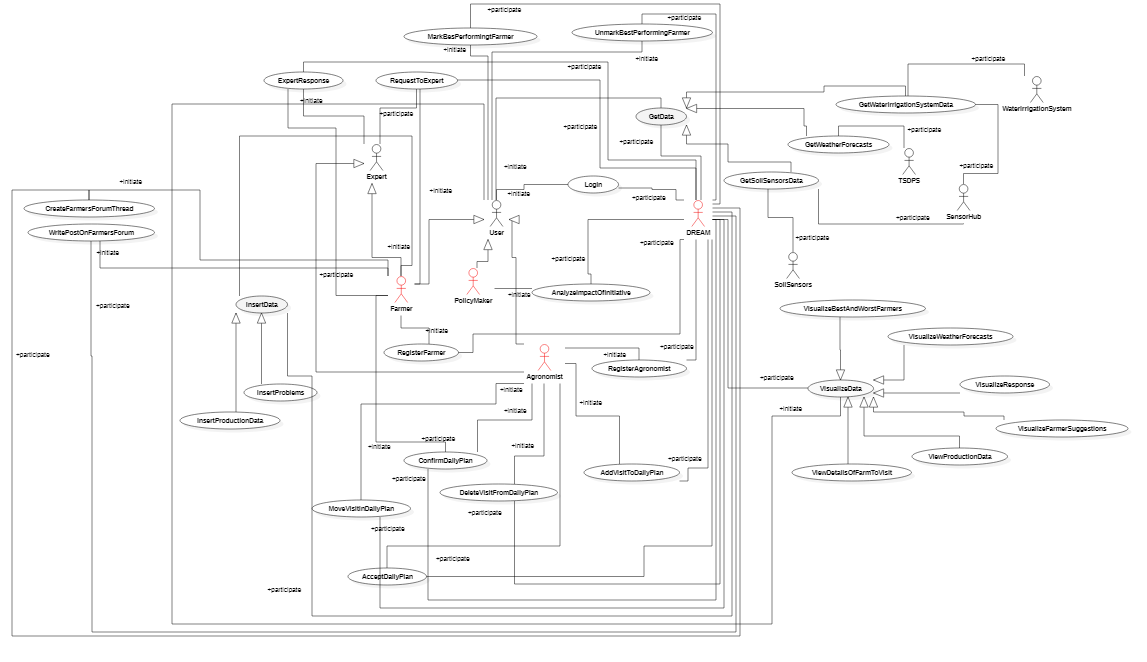
\includegraphics[scale=0.75]{use cases model/use cases model.png}
    \caption{This is the use cases model of the system.}
\end{sidewaysfigure}
\clearpage
\newpage
%%%%%%%%%%%%%%%%%%%%%%%%%%%%TABLE 1%%%%%%%%%%%%%%%%%%%%%%%
%\rowcolors{2}{blue!15}{blue!25}
\centering
\begin{longtable}{|p{3.5cm}|m{8cm}|}
 \caption{Use case 1: RegisterFarmer}
 \label{uc1}
 \hline
 \multicolumn{2}{|c|}{\cellcolor{white}\emph{USE CASE 1}} \\
  % do not write anything here
 \endfirsthead
 % do not write anything here
 \endhead
 % do not write anything here
 \endfoot
 % do not write anything here
 \endlastfoot
 \hline
 Name & RegisterFarmer\\
 \hline
 Actor & Farmer\\
 \hline
 Entry condition & The farmer does not have an account and wants to enrol in the \verb|DREAM| system.\\
 \hline
 Event flow & \begin{enumerate}
    \item The farmer accesses to the \verb|DREAM| landing page.
    \item \verb|DREAM| shows a form for logging in and a button "Sign Up Farmer".
    \item The farmer selects the "Sign Up Farmer" button.
    \item \verb|DREAM| shows a form to insert the farmer's personal data (name, surname, birthdate), his/her e-mail, a password and the location of his/her farm.
    \item The farmer inserts his name, surname, birthdate, e-mail, password and the location of his/her farm.
    \item The farmer clicks on the "Sign Up" button.
    \item \verb|DREAM| checks the validity of the data, and then it sends an e-mail to the inserted e-mail address, containing a confirmation link to complete the enrolling.
    \item \verb|DREAM| shows a message advising the farmer to check his e-mail and click on the confirm link. 
    \item The farmer clicks on the confirm link sent in the e-mail.
 \end{enumerate}\\
 \hline
 Exit condition & \verb|DREAM| shows a confirm of having created the account correctly and a link to the farmer's homepage.\\
 \hline
 Exceptions & \begin{itemize}
     \item If the e-mail inserted by the farmer is already used in the \verb|DREAM| system, an error message is shown.
     \item If one of the data inserted by the farmer is empty, an error message is shown.
     \item If the password is shorter than 10 characters, an error message is shown.
     \item If the farmer 24 hours after having inserted his data has not clicked on the confirm link, the signing up process is canceled and if the farmer clicks on the link an error message is shown.
 \end{itemize}\\
 \hline
 Special requirements &
 \begin{itemize}
     \item The e-mail with the confirm link should be sent by \verb|DREAM| in less than 10 seconds.
     \item After the farmer has clicked on the confirm link, the confirm message should be shown in less than 3 seconds.
 \end{itemize}\\
 \hline
\end{longtable}

\begin{figure}[H]
    \centering
    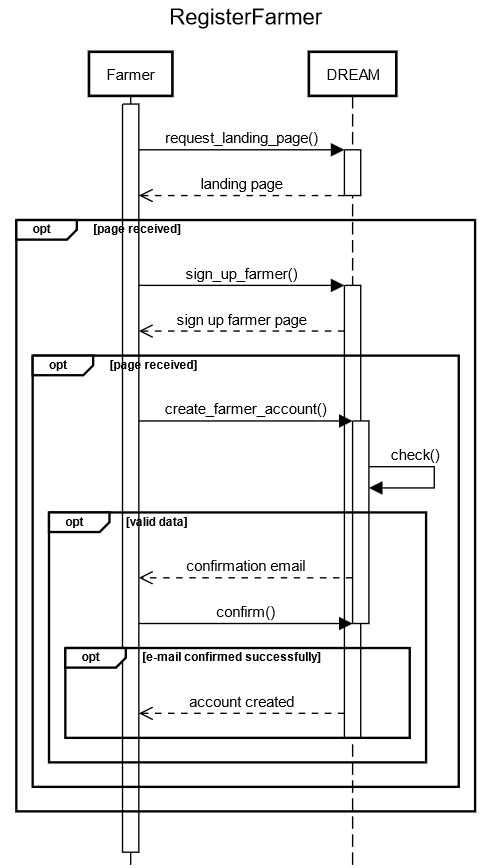
\includegraphics[scale=0.60]{sequence_diagrams/RegisterFarmer.png}
    \caption{Sequence diagram for the RegisterFarmer use case.}
\end{figure}
\newpage
%%%%%%%%%%%%%%%%%%%%%%%%%%%%TABLE 2%%%%%%%%%%%%%%%%%%%%%%%

\centering
\begin{longtable}{|p{3.5cm}|m{8cm}|}
\caption{Use case 2: RegisterAgronomist}
 \label{uc2}
 \hline
 \multicolumn{2}{|c|}{\cellcolor{white}\emph{USE CASE 2}} \\
  % do not write anything here
 \endfirsthead
 % do not write anything here
 \endhead
 % do not write anything here
 \endfoot
 % do not write anything here
 \endlastfoot
 \hline
 Name & RegisterAgronomist\\
 \hline
 Actor & Agronomist\\
 \hline
 Entry condition & The agronomist logs in the \verb|DREAM| system for the first time with the credentials he has already received.\\
 \hline
 Event flow & \begin{enumerate}
    \item \verb|DREAM| shows a form for inserting the agronomist's personal and working data (name, surname, birthdate, optionally a specialization) and the area he is reponsible of.
    \item The agronomist inserts his personal and working data.
    \item The agronomist selects the area he is responsible of.
    \item The agronomist clicks on the "Done" button.
 \end{enumerate}\\
 \hline
 Exit condition & The agronomist is shown the agronomist's homepage of the \verb|DREAM| system.\\
 \hline
 Exceptions & \begin{itemize}
     \item If the agronomist inserts an empty name, surname or birthdate, an error is shown.
     \item If the agronomist does not select the area which he/she is assigned to, an error is shown.
 \end{itemize}\\
 \hline
 Special requirements & \begin{itemize}
     \item After clicking on the "Done" button, the agronomist must be shown the homepage in less than 3 seconds.
 \end{itemize}\\
 \hline
\end{longtable}

\begin{figure}[H]
    \centering
    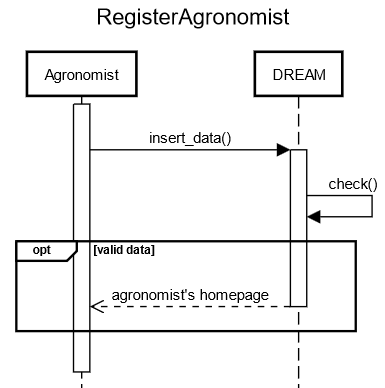
\includegraphics[scale=0.60]{sequence_diagrams/RegisterAgronomist}
    \caption{Sequence diagram for the RegisterAgronomist use case.}
\end{figure}
\newpage
%%%%%%%%%%%%%%%%%%%%%%%%%%%%TABLE 3%%%%%%%%%%%%%%%%%%%%%%%

\centering
\begin{longtable}{|p{3.5cm}|m{8cm}|}
\caption{Use case 3: LogIn}
 \label{uc3}
 \hline
 \multicolumn{2}{|c|}{\cellcolor{white}\emph{USE CASE 3}} \\
  % do not write anything here
 \endfirsthead
 % do not write anything here
 \endhead
 % do not write anything here
 \endfoot
 % do not write anything here
 \endlastfoot
 \hline
 Name & LogIn\\
 \hline
 Actor & User (either a Farmer, an Agronomist or a Policy Maker)\\
 \hline
 Entry condition & The user is not logged in the system and wants to log in.\\
 \hline
 Event flow & \begin{enumerate}
    \item The user accesses to the \verb|DREAM| landing page.
    \item \verb|DREAM| shows a form for logging in.
    \item The user inserts his/her e-mail, password and selects his role (either farmer, agronomist or policy maker).
    \item The user clicks on the "Log In" button. 
 \end{enumerate}\\
 \hline
 Exit condition & The user is logged in and is shown the homepage of the \verb|DREAM| system.\\
 \hline
 Exceptions & \begin{itemize}
     \item If the credentials inserted by the user are not correct, an error message is shown on the landing page and the log in is not allowed.
 \end{itemize}\\
 \hline
 Special requirements & \begin{itemize}
     \item After clicking on the "Log In" button, the user must be shown the homepage in less than 3 seconds.
 \end{itemize}\\
 \hline
\end{longtable}

\begin{figure}[H]
    \centering
    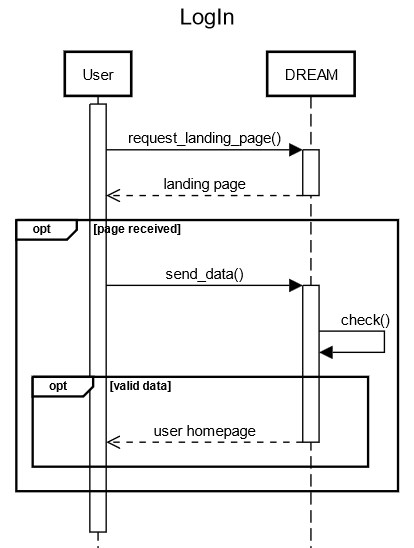
\includegraphics[scale=0.60]{sequence_diagrams/LogIn.png}
    \caption{Sequence diagram for the LogIn use case.}
\end{figure}

\newpage
%%%%%%%%%%%%%%%%%%%%%%%%%%%%TABLE 4%%%%%%%%%%%%%%%%%%%%%%%

\centering
\begin{longtable}{|p{3.5cm}|m{8cm}|}
\caption{Use case 4: ViewProductionData}
 \label{uc4}
 \hline
 \multicolumn{2}{|c|}{\cellcolor{white}\emph{USE CASE 4}} \\
  % do not write anything here
 \endfirsthead
 % do not write anything here
 \endhead
 % do not write anything here
 \endfoot
 % do not write anything here
 \endlastfoot
 \hline
 Name & ViewProductionData\\
 \hline
 Actor & Farmer\\
 \hline
 Entry condition & The farmer is logged in the \verb|DREAM| system and wants to visualize his/her past production data.\\
 \hline
 Event flow & \begin{enumerate}
    \item The farmer selects the "My Productions" entry in the homepage.
    \item \verb|DREAM| shows a list of production data items, each one of them containing a date and the corresponding activities performed by the farmer in that date (seeding, planting, fertilizing, watering and harvesting) with the relative details, the comments about these activities inserted by the farmer and, potentially, the problems inserted by the farmer relative to that date Moreover, an "Insert Production Data" button and a "Select Dates" form are shown.
    \item The farmer inserts in the "Select Dates" form the start and end date for which he/she wants to visualize his production data.
    \item The farmer clicks on the "Select Dates" button.
 \end{enumerate}\\
 \hline
 Exit condition & The user is shown a list of production data relative to the dates between the start and end dates - included - inserted.\\
 \hline
 Exceptions & \begin{itemize}
     \item If no production data are relative to the inserted start and and dates, a warning message is shown.
 \end{itemize}\\
 \hline
 Special requirements & \begin{itemize}
     \item After clicking on the "My Production" button, the user must be shown the view in less than 3 seconds.
     \item After clicking on the "Select Dates" button, the user must be shown the view in less than 3 seconds.
 \end{itemize}\\
 \hline
\end{longtable}

\begin{figure}[H]
    \centering
    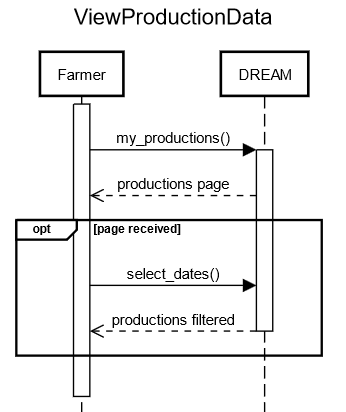
\includegraphics[scale=0.60]{sequence_diagrams/ViewProductionData.png}
    \caption{Sequence diagram for the ViewProductionData use case.}
\end{figure}
\newpage
%%%%%%%%%%%TABLE 5%%%%%%%%%%%%%%%%%%%%%%%%%%%%%%%%%%%%%%%%

\centering
\begin{longtable}{|p{3.5cm}|m{8cm}|}
\caption{Use case 5: InsertProductionData}
 \label{uc5}
 \hline
 \multicolumn{2}{|c|}{\cellcolor{white}\emph{USE CASE 5}} \\
  % do not write anything here
 \endfirsthead
 % do not write anything here
 \endhead
 % do not write anything here
 \endfoot
 % do not write anything here
 \endlastfoot
 \hline
 Name & InsertProductionData\\
 \hline
 Actor & Farmer\\
 \hline
 Entry condition & The farmer wants to insert some data about his/her production activity. He/she is already logged in the \verb|DREAM| system.\\
 \hline
 Event flow & \begin{enumerate}
    \item In the homepage, the farmer selects from the menu the item "My Production".
    \item \verb|DREAM| shows a list of production data items and a "Insert Production Data" button.
    \item The farmer clicks on the "Insert Production Data" button.
    \item \verb|DREAM| shows a form that allows the farmer to insert the date the production data is referred to; for each of his plantations, the actions (seeding, planting, fertilizing, watering, harvesting) the farmer has performed on a single day of work and for each action some more details (for seeding, planting and harvesting the quantity of product involved, for fertilizing the type and quantity of the fertilizer used , for watering the amount of water used). Moreover, the farmer can also insert a textual description of the activity performed.
    \item The farmer inserts the date which the production data are referred to.
    \item For each product type, the farmer selects the action(s) he performed and the details related to that action(s).
    \item Optionally, the farmer inserts a brief description of the activity performed or some observations about it.
    \item The farmer clicks on the "Insert" button.
    \item \verb|DREAM| checks the validity of the data.
    \color{black}
 \end{enumerate}\\
 \hline
 Exit condition & The farmer is shown a confirm of having inserted the data into the system together with the data just inserted.\\
 \hline
 Exceptions & \begin{itemize}
     \item If the kind of product is not present, the farmer can add the new product together with the area dedicated to it.
 \end{itemize}\\
 \hline
 Special requirements & \begin{itemize}
     \item When the farmer clicks on the "Insert" button, the confirmation is shown in less than 3 seconds.
 \end{itemize}\\
 \hline
\end{longtable}

\begin{figure}[H]
    \centering
    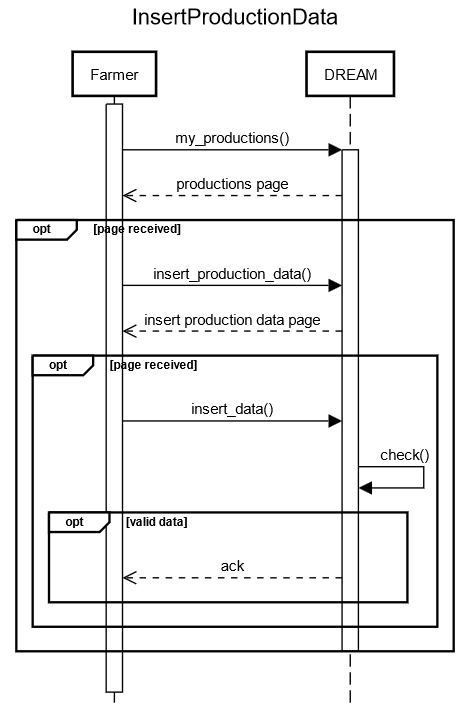
\includegraphics[scale=0.75]{sequence_diagrams/InsertProductionData.png}
    \caption{Sequence diagram for the InsertProductionData use case.}
\end{figure}
\newpage
%%%%%%%%%%%TABLE 6%%%%%%%%%%%%%%%%%%%%%%%%%%%%%%%%%%%%%%%%

\begin{longtable}{|p{3.5cm}|m{8cm}|}
\caption{Use case 6: InsertProblems}
 \label{uc6}
 \hline
 \multicolumn{2}{|c|}{\cellcolor{white}\emph{USE CASE 6}} \\
 % do not write anything here
 \endfirsthead
 % do not write anything here
 \endhead
 % do not write anything here
 \endfoot
 % do not write anything here
 \endlastfoot
 \hline
 Name & InsertProblems\\
 \hline
 Actor & Farmer\\
 \hline
 Entry condition & The farmer faces a problem and decides to communicate it on \verb|DREAM|. He/she is already logged in the \verb|DREAM| system.\\
 \hline
 Event flow & \begin{enumerate}
    \item In the homepage, the farmer selects from the menu the item "Insert Problem".
    \item \verb|DREAM| shows a form to insert a problem.
    \item The farmer selects the kind of problem among a list of available ones, when the problem occurred and how much it lasted.
    \item The farmer gives a brief description of the problem.
    \item The farmer selects whether he would like to meet as soon as possible an agronomist.
    \item The farmer clicks on the "Insert" button.
    \color{black}
 \end{enumerate}\\
 \hline
 Exit condition & The farmer is shown the problem he inserted with a confirm of having successfully inserted it into the system.
 If the farmer requested a visit from an agronomist, an agronomist assigned to the area of the farmer is scheduled the visit in his daily plan during the following days and the farmer is notified about the date and time of the visit.\\
 \hline
 Exceptions & \begin{itemize}
     \item If the kind of problem is not present, the farmer can add it by its own.
     \item In case no agronomist can be scheduled for the current week, the farmer is notified about the problem and an agronomist will be found for the next week.
 \end{itemize}\\
 \hline
 Special requirements & \begin{itemize}
     \item After the farmer clicks on the "send" button, the problem is inserted in the system (and the visit of the agronomist is scheduled, if requested) in less than 3 seconds.
 \end{itemize}\\
 \hline
\end{longtable}
\begin{figure}[H]
    \centering
    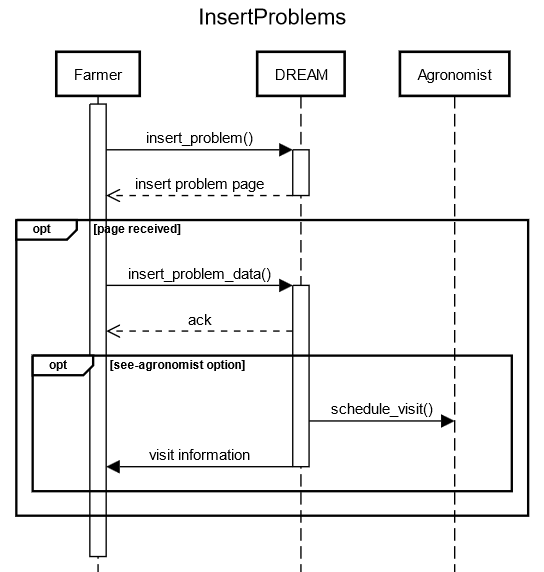
\includegraphics[scale=0.75]{sequence_diagrams/InsertProblems}
    \caption{Sequence diagram for the InsertProblems use case}
\end{figure}
\newpage
%%%%%%%%%%%%%%%%%%%%%%%%%%%%TABLE 7%%%%%%%%%%%%%%%%%%%%%%%

\centering
\begin{longtable}{|p{3.5cm}|m{8cm}|}
\caption{Use case 7: AcceptDailyPlan}
 \label{uc7}
 \hline
 \multicolumn{2}{|c|}{\cellcolor{white}\emph{USE CASE 7}} \\
  % do not write anything here
 \endfirsthead
 % do not write anything here
 \endhead
 % do not write anything here
 \endfoot
 % do not write anything here
 \endlastfoot
 \hline
 Name & AcceptDailyPlan\\
 \hline
 Actor & Agronomist\\
 \hline
 Entry condition & The agronomist is logged in the \verb|DREAM| system and wants to visualize the daily plan for the next working day, which he has not accepted yet.\\
 \hline
 Event flow & \begin{enumerate}
    \item The agronomist accesses the "Daily Plan" area from the homepage.
    \item \verb|DREAM| shows a list of 7 dates, starting with the present day and including only working days.
    \item The agronomist selects the date of his/her next working day.
    \item \verb|DREAM| shows the daily plan of the agronomist for the selected date: it is a list of visits to farms. For each visit, the name and surname of the farmer, the location of the farm, the starting hour of the visit are shown; and there are a "Farm Details" button (view UC8 for more details), a "Move" button (view UC9 for more details) and a "Delete" button (view UC10 for more details). Moreover, an "Add Visit" button (view UC11 for more details) and a "Accept Daily Plan" button are present.
    \item After possibly visualizing details about the farms to visit (UC8) or modifying the daily plan (UC9, UC10, UC11), the agronomist clicks on the "Accept Daily Plan button"
 \end{enumerate}\\
 \hline
 Exit condition & The agronomist is shown the daily plan for the selected date without the "Move", "Delete", "Add Visit" and "Accept Daily Plan" buttons, and all the farmers involved in the visits in the accepted daily plan are notified about the visit.\\
 \hline
 Exceptions & \begin{itemize}
     \item If the agronomist has modified the daily plan and the daily plan is not acceptable, the daily plan is shown to the agronomist with all the buttons to modify it, together with an error message.
 \end{itemize}\\
 \hline
 Special requirements &\begin{itemize}
     \item When selecting the daily plan date, the agronomist must be shown the daily plan in less than 3 seconds.
 \end{itemize}\\
 \hline
\end{longtable}

\begin{figure}[H]
    \centering
    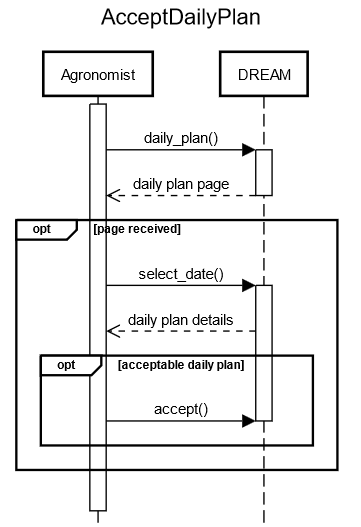
\includegraphics[scale=0.75]{sequence_diagrams/AcceptDailyPlan.png}
    \caption{Sequence diagram for the AcceptDailyPlan use case.}
\end{figure}
\newpage
%%%%%%%%%%%%%%%%%%%%%%%%%%%%TABLE 8%%%%%%%%%%%%%%%%%%%%%%%

\centering
\begin{longtable}{|p{3.5cm}|m{8cm}|}
\caption{Use case 8: ViewDetailsOfFarmToVisit}
 \label{uc8}
 \hline
 \multicolumn{2}{|c|}{\cellcolor{white}\emph{USE CASE 8}} \\
  % do not write anything here
 \endfirsthead
 % do not write anything here
 \endhead
 % do not write anything here
 \endfoot
 % do not write anything here
 \endlastfoot
 \hline
 Name & ViewDetailsOfFarmToVisit\\
 \hline
 Actor & Agronomist\\
 \hline
 Entry condition & The agronomist is logged in the \verb|DREAM| system and is visualizing the daily plan of a certain work day. He/She wants to see more details about a farm present in the daily plan.\\
 \hline
 Event flow & \begin{enumerate}
    \item The agronomist clicks on the "Farm Details" button relative to a farm to visit.
    \item \verb|DREAM| shows a list of production data items and a list of problems inserted by the farmer owning the farm to visit, starting from the day after the last visit of the agronomist (or from the subscription of the farmer into the system, if the agronomist has never visited the farmer) until the present day.
 \end{enumerate}\\
 \hline
 Exit condition & The agronomist can read the details about the farmer, and clicking on a "Back" button, returning to the daily plan view.\\
 \hline
 Exceptions & \begin{itemize}
     \item If there are no production data relative to the farm, a message is shown.
     \item If there are no problems relative to the farm, a message is shown.
 \end{itemize}\\
 \hline
 Special requirements &\begin{itemize}
     \item When selecting the "Farm Details" button, the agronomist must be shown the farm details in less than 3 seconds.
 \end{itemize}\\
 \hline
\end{longtable}

\begin{figure}[H]
    \centering
    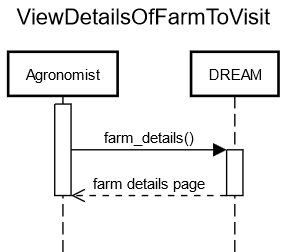
\includegraphics[scale=0.75]{sequence_diagrams/ViewDetailsOfFarmToVisit.png}
    \caption{Sequence diagram for the ViewDetailsOfFarmToVisit use case.}
\end{figure}
\newpage
%%%%%%%%%%%%%%%%%%%%%%%%%%%%TABLE 9%%%%%%%%%%%%%%%%%%%%%%%

\centering
\begin{longtable}{|p{3.5cm}|m{8cm}|}
\caption{Use case 9: MoveVisitInDailyPlan}
 \label{uc9}
 \hline
 \multicolumn{2}{|c|}{\cellcolor{white}\emph{USE CASE 9}} \\
  % do not write anything here
 \endfirsthead
 % do not write anything here
 \endhead
 % do not write anything here
 \endfoot
 % do not write anything here
 \endlastfoot
 \hline
 Name & MoveVisitInDailyPlan\\
 \hline
 Actor & Agronomist\\
 \hline
 Entry condition & The agronomist is logged in the \verb|DREAM| system and is visualizing the daily plan of a certain work day. He/She wants to move a visit from a starting hour to another one, either because the work day is ended and he/she performed the visit in a different hour than the selected one or because he/she wants to modify the daily plan for a future work day before accepting it.\\
 \hline
 Event flow & \begin{enumerate}
    \item The agronomist clicks on the "Move" button relative to a certain visit.
    \item \verb|DREAM| shows an input field for inserting the starting hour of the visit and an "Insert" button.
    \item The agronomist inserts the starting hour of the visit.
    \item The agronomist clicks on the "Insert" button.
 \end{enumerate}\\
 \hline
 Exit condition & The agronomist is shown the daily plan of the work day, exactly like it was before the update, except for the fact that the starting date of the selected visit has been updated with the inserted one\\
 \hline
 Exceptions & \begin{itemize}
     \item If the inserted starting date is outside the working hours of the agronomist, the daily plan is not updated and an error message is shown.
 \end{itemize}\\
 \hline
 Special requirements &\begin{itemize}
     \item When selecting the "Insert" button, the agronomist must be shown the updated daily plan in less than 3 seconds.
 \end{itemize}\\
 \hline
\end{longtable}

\begin{figure}[H]
    \centering
    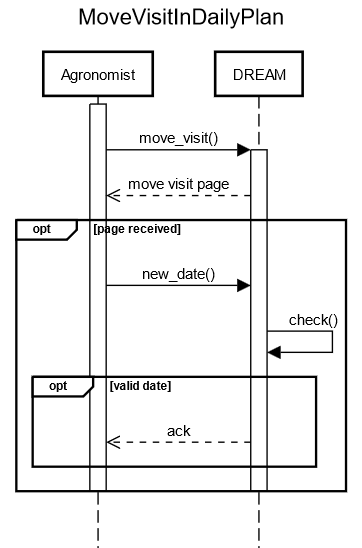
\includegraphics[scale=0.75]{sequence_diagrams/MoveVisitInDailyPlan.png}
    \caption{Sequence diagram for the MoveVisitInDailyPlan use case.}
\end{figure}
\newpage
%%%%%%%%%%%%%%%%%%%%%%%%%%%%TABLE 10%%%%%%%%%%%%%%%%%%%%%%%

\centering
\begin{longtable}{|p{3.5cm}|m{8cm}|}
\caption{Use case 10: DeleteVisitFromDailyPlan}
 \label{uc10}
 \hline
 \multicolumn{2}{|c|}{\cellcolor{white}\emph{USE CASE 10}} \\
  % do not write anything here
 \endfirsthead
 % do not write anything here
 \endhead
 % do not write anything here
 \endfoot
 % do not write anything here
 \endlastfoot
 \hline
 Name & DeleteVisitFromDailyPlan\\
 \hline
 Actor & Agronomist\\
 \hline
 Entry condition & The agronomist is logged in the \verb|DREAM| system and is visualizing the daily plan of a certain work day. He/She wants to delete a visit, either because the work day is ended and he/she did not perform the visit or because he/she wants to modify the daily plan for a future work day before accepting it.\\
 \hline
 Event flow & \begin{enumerate}
    \item The agronomist clicks on the "Delete" button relative to a certain visit.
 \end{enumerate}\\
 \hline
 Exit condition & The agronomist is shown the daily plan of the work day, exactly like it was before the update, except for the fact that the selected visit has been deleted.\\
 \hline
 Exceptions & - \\
 \hline
 Special requirements &\begin{itemize}
     \item When selecting the "Delete" button, the agronomist must be shown the updated daily plan in less than 3 seconds.
 \end{itemize}\\
 \hline
\end{longtable}

\begin{figure}[H]
    \centering
    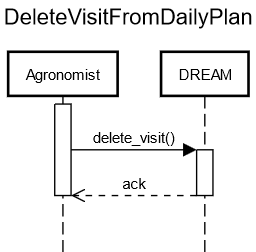
\includegraphics[scale=0.75]{sequence_diagrams/DeleteVisitFromDailyPlan.png}
    \caption{Sequence diagram for the DeleteVisitFromDailyPlan use case.}
\end{figure}
\newpage
%%%%%%%%%%%%%%%%%%%%%%%%%%%%TABLE 11%%%%%%%%%%%%%%%%%%%%%%%

\centering
\begin{longtable}{|p{3.5cm}|m{8cm}|}
\caption{Use case 11: AddVisitToDailyPlan}
 \label{uc11}
 \hline
 \multicolumn{2}{|c|}{\cellcolor{white}\emph{USE CASE 11}} \\
  % do not write anything here
 \endfirsthead
 % do not write anything here
 \endhead
 % do not write anything here
 \endfoot
 % do not write anything here
 \endlastfoot
 \hline
 Name & AddVisitToDailyPlan\\
 \hline
 Actor & Agronomist\\
 \hline
 Entry condition & The agronomist is logged in the \verb|DREAM| system and is visualizing the daily plan of a certain work day. He/She wants to add a visit to the plan, either because the work day is ended and he/she performed a visit which was not planned or because he/she wants to modify the daily plan for a future work day before accepting it.\\
 \hline
 Event flow & \begin{enumerate}
    \item The agronomist clicks on the "Add Visit" button.
    \item \verb|DREAM| shows a list of all farmers in the area of the agronomist and an input field for the starting hour of the visit.
    \item The agronomist selects a farmer from the list of farmers.
    \item The agronomist inserts a starting hour for the visit.
    \item The agronomist clicks on the "Add" button.
 \end{enumerate}\\
 \hline
 Exit condition & The agronomist is shown the daily plan of the work day, exactly like it was before the update, except for the fact that the new visit has been added.\\
 \hline
 Exceptions & \begin{itemize}
     \item If the inserted starting date is outside the working hours of the agronomist, the daily plan is not updated and an error message is shown.
 \end{itemize}\\
 \hline
 Special requirements &\begin{itemize}
     \item When selecting the "Add" button, the agronomist must be shown the updated daily plan in less than 3 seconds.
 \end{itemize}\\
 \hline
\end{longtable}

\begin{figure}[H]
    \centering
    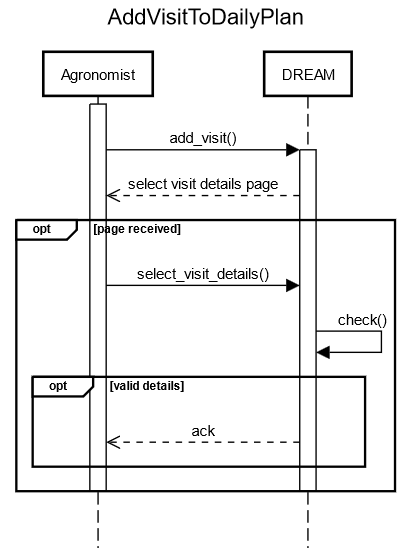
\includegraphics[scale=0.75]{sequence_diagrams/AddVisitToDailyPlan.png}
    \caption{Sequence diagram for the AddVisitToDailyPlan use case.}
\end{figure}
\newpage
%%%%%%%%%%%%%%%%%%%%%%%%%%%%TABLE 12%%%%%%%%%%%%%%%%%%%%%%%

\centering
\begin{longtable}{|p{3.5cm}|m{8cm}|}
\caption{Use case 12: ConfirmDailyPlan}
 \label{uc12}
 \hline
 \multicolumn{2}{|c|}{\cellcolor{white}\emph{USE CASE 12}} \\
  % do not write anything here
 \endfirsthead
 % do not write anything here
 \endhead
 % do not write anything here
 \endfoot
 % do not write anything here
 \endlastfoot
 \hline
 Name & ConfirmDailyPlan\\
 \hline
 Actor & Agronomist\\
 \hline
 Entry condition & The working day of an agronomist has ended - more precisely, it is passed at least half an hour from the starting hour of the last visit planned for the agronomist  - and the agronomist, who is already logged in the system, wants to confirm the daily plan of the day, possibly specifying some deviations.\\
 \hline
 Event flow & \begin{enumerate}
    \item The agronomist accesses the "Daily Plan" area from the homepage.
    \item \verb|DREAM| shows a list of 7 dates, starting with the present day and including only working days.
    \item The agronomist selects the date of the present work day.
    \item \verb|DREAM| shows the daily plan of the agronomist for the present work day. For each visit, the name and surname of the farmer, the location of the farm, the starting hour of the visit are shown; and there are a "Farm Details" button (view UC8 for more details), a "Move" button (view UC9 for more details), a "Delete" button (view UC10 for more details) and an input field for inserting a report about the visit. Moreover, an "Add Visit" button (view UC11 for more details) and a "Confirm Daily Plan" button are present.
    \item The agronomist writes the reports for all the visits performed.
    \item After possibly visualizing details about the farms to visit (UC8) or modifying the daily plan (UC9, UC10, UC11), the agronomist clicks on the "Confirm Daily Plan button"
 \end{enumerate}\\
 \hline
 Exit condition & The agronomist is shown the daily plan for the present work day without the "Move", "Delete", "Add Visit", "Insert Report" and "Confirm Daily Plan" buttons. \\
 \hline
 Exceptions & \begin{itemize}
     \item If the agronomist does not insert the report (UC13) for one of the performed visits, an error message is shown and the system does not let the agronomist confirm the plan.
     \item If the agronomist does not confirm the daily plan during the present day, the "Daily Plan" page will contain in the list of dates for the daily plans also the date of the unconfirmed daily plan, together with a message warning the agronomist to confirm the daily plan.
 \end{itemize}\\
 
 \hline
 Special requirements & After having selected the "Confirm Daily Plan" button, the agronomist must be shown the daily plan in less than 3 seconds.\\
 \hline
\end{longtable}

\begin{figure}[H]
    \centering
    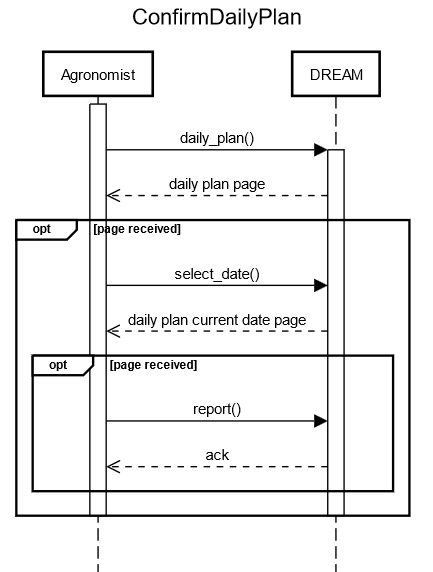
\includegraphics[scale=0.75]{sequence_diagrams/ConfirmDailyPlan.png}
    \caption{Sequence diagram for the ConfirmDailyPlan use case.}
\end{figure}

\newpage
%%%%%%%%%%%%%%%%%%%%%%%%%%%%TABLE 13%%%%%%%%%%%%%%%%%%%%%%%

\centering
\begin{longtable}{|p{3.5cm}|m{8cm}|}
\caption{Use case 13: GetSoilSensorsData}
 \label{uc13}
 \hline
 \multicolumn{2}{|c|}{\cellcolor{white}\emph{USE CASE 13}} \\
  % do not write anything here
 \endfirsthead
 % do not write anything here
 \endhead
 % do not write anything here
 \endfoot
 % do not write anything here
 \endlastfoot
 \hline
 Name & GetSoilSensorsData\\
 \hline
 Actor & SoilSensorsHub\\
 \hline
 Entry condition & It is 06:00, or 14:00, or 22:00 \footnote{All times are referred to the UTC+5:30 time zone, which is the one used in India}.\\
 \hline 
 Event flow & \begin{enumerate}
    \item \verb|DREAM| sends the SoilSensorsrHub a request for data about soil moisture.
    \item The SoilSensorsHub replies with a list of $<$sensorId, currentSoilMoisture$>$ items, one for each sensor managed by the hub.
 \end{enumerate}\\
 \hline
 Exit condition & \verb|DREAM| either receives the data or the maximum number of attempts is reached.\\
 \hline
 Exceptions & \begin{itemize}
     \item In case the SoilSensorsHub is not reachable, \verb|DREAM| retries to contact it 3 times, with an interval of 30 minutes between them; if after the third try the SoilSensorsHub has not been contacted successfully yet, \verb|DREAM| will contact it in 6:30 hours (that is, at the next scheduled time for contact the SoilSensorsHub).
 \end{itemize}\\
 \hline
 Special requirements & -\\
 \hline
\end{longtable}

\begin{figure}[H]
    \centering
    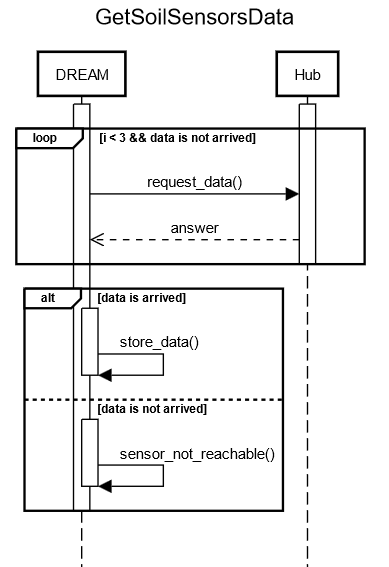
\includegraphics[scale=0.75]{sequence_diagrams/GetSoilSensorsData}
    \caption{Sequence diagram for the GetSoilSensorsData use case.}
\end{figure}
\newpage

%%%%%%%%%%%%%%%%%%%%%%%%%%%%TABLE 14%%%%%%%%%%%%%%%%%%%%%%%

\centering
\begin{longtable}{|p{3.5cm}|m{8cm}|}
\caption{Use case 14: GetWaterIrrigationSystemData}
 \label{uc14}
 \hline
 \multicolumn{2}{|c|}{\cellcolor{white}\emph{USE CASE 14}} \\
  % do not write anything here
 \endfirsthead
 % do not write anything here
 \endhead
 % do not write anything here
 \endfoot
 % do not write anything here
 \endlastfoot
 \hline
 Name & GetWaterIrrigationSystemData\\
 \hline
 Actor & WaterIrrigationSystem\\
 \hline
 Entry condition & It is 00:00. \footnote{Time referred to the UTC+5:30 time zone}\\
 \hline
 Event flow & \begin{enumerate}
    \item \verb|DREAM| requests the WaterIrrigationSystem for the data relative to the day which has just ended.
    \item The WaterIrrigationSystem replies with a list of $<$deviceId, waterUsedAmount$>$ items, one for each water irrigation device managed by the WaterIrrigationSystem.
 \end{enumerate}\\
 \hline
 Exit condition & \verb|DREAM| will send the next request to the WaterIrrigationSystem in 24 hours.\\
 \hline
 Exceptions & \begin{itemize}
     \item In case the WaterIrrigationSystem is not reachable, \verb|DREAM| retries to contact it 3 times, with an interval of 30 minutes between them; if after the third try the WaterIrrigationSystem has not been contacted successfully yet, \verb|DREAM| will contact the next day at 00:00.
 \end{itemize}\\
 \hline
 Special requirements &\begin{itemize}
     -
 \end{itemize}\\
 \hline
\end{longtable}
\begin{figure}[H]
    \centering
    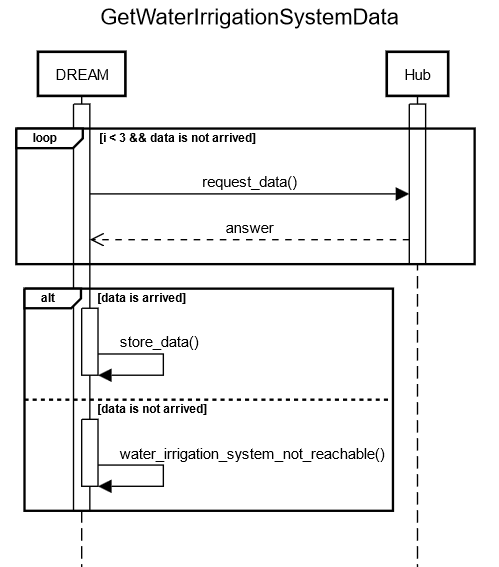
\includegraphics[scale=0.75]{sequence_diagrams/GetWaterIrrigationSystemData}
    \caption{Sequence diagram for the GetWaterIrrigationSystemData use case}
\end{figure}
\newpage
%%%%%%%%%%%%%%%%%%%%%%%%%%%%TABLE 15%%%%%%%%%%%%%%%%%%%%%%%

\centering
\begin{longtable}{|p{3.5cm}|m{8cm}|}
\caption{Use case 15: VisualizeBestAndWorstFarmers}
 \label{uc15}
 \hline
 \multicolumn{2}{|c|}{\cellcolor{white}\emph{USE CASE 15}} \\
  % do not write anything here
 \endfirsthead
 % do not write anything here
 \endhead
 % do not write anything here
 \endfoot
 % do not write anything here
 \endlastfoot
 \hline
 Name & VisualizeBestAndWorstFarmers\\
 \hline
 Actor & Policy Maker, TSDPSSystem\\
 \hline
 Entry condition & The policy maker is logged in the system and wants to visualize best and worst performing farmers according to some certain criteria.\\
 \hline
 Event flow & \begin{enumerate}
    \item From the homepage, the policy maker accesses the Farms section.
    \item \verb|DREAM| shows:
    \begin{itemize}
        \item a form for selecting one or more criteria to rank the farmers;
        \item a form for (optionally) inserting some weights associated to these criteria;
        \item a form for (optionally) inserting the number N of best farmers and the number M of worst farmers to display according to the selected criterion;
        \item a form for (optionally) selecting the area of the farmers to consider;
        \item a form for (optionally) selecting the time period to consider for ranking the farmers.
    \end{itemize}
    \item The policy maker selects one or more criteria to rank the farmers among the list of available ones.
    \item Optionally, the policy maker inserts some weights associated to the selected criteria.
    \item Optionally, the policy maker inserts the number N of best farmers to display.
    \item Optionally, the policy maker inserts the number M of worst farmers to display.
    \item Optionally, the policy maker selects the area where the farms to rank should be located.
    \item Optionally, the policy maker inserts the start and end date of the period to consider for ranking the farmers.
    \item The policy maker clicks on the "Rank" button.
    \item Depending on the criteria selected, \verb|DREAM| may fetch from the TSDPSSystem some data from the weather reports (view UC23 for more details)
 \end{enumerate}\\
 \hline
 Exit condition & If no limits on the number of farmers to display were inserted, \verb|DREAM| shows a list of all farmers (belonging to the selected area, if there was one) ordered according to the selected criteria, together with a "Mark As Best-Performing" button for each farmer in the first half of the list and a "Mark As Worst-Performing" button in the second half of the list. \newline
 If limits on the farmers to display were specified, \verb|DREAM| shows the list of the first N farmers and the list of the last M farmers according to the selected criteria (and belonging to the selected area, if there was one). For each farmer in the first list, there is a "Mark As Best-Performing" button; for each farmer in the latter list, there is a "Mark As Worst-Performing" button.
 \newline
 In both cases, if farmer was already marked as best- or worst-performing, the "Mark As Best-Performing" and "Mark As Worst-Performing" are not present, and there is a flag that shows that they are already marked, and a button "Unmark".
 \newline
 Moreover, for each farmer there is a "FarmDetails" button. By clicking on it, the policy maker can see a table with monthly seeded, planted, watered, fertilized and harvested amounts for each crop grown in the farm.\\
 \hline
 Exceptions & \begin{itemize}
    \item If there is no data in the system about farmers that respect the constraints selected by the policy maker (area and time period), a warning message is displayed.
 \end{itemize}\\
 \hline
 Special requirements &\begin{itemize}
     \item After the policy maker clicks on the "Rank" button, the lists should be shown in at most 10 seconds.
 \end{itemize}\\
 \hline
\end{longtable}

\begin{figure}[H]
    \centering
	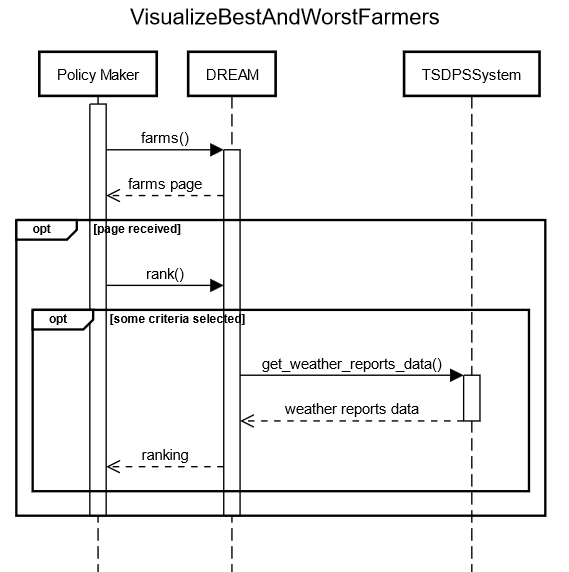
\includegraphics[scale=0.5]{sequence_diagrams/VisualizeBestAndWorstFarmers.png}
    \caption{Sequence diagram for the VisualizeBestAndWorstFarmers use case.}
\end{figure}
OBS.: The use case for the agronomist is almost equivalent to this one; the only difference is that an agronomist is not allowed to choose the area of the farmers to consider, as the farmers he/she can visualize are only the ones located in the area the agronomist is assigned to (event 7 not present).
\newpage
%%%%%%%%%%%%%%%%%%%%%%%%%%%%TABLE 16%%%%%%%%%%%%%%%%%%%%%%%

\centering
\begin{longtable}{|p{3.5cm}|m{8cm}|}
\caption{Use case 16: MarkBestPerformingFarmer}
 \label{uc16}
 \hline
 \multicolumn{2}{|c|}{\cellcolor{white}\emph{USE CASE 16}} \\
  % do not write anything here
 \endfirsthead
 % do not write anything here
 \endhead
 % do not write anything here
 \endfoot
 % do not write anything here
 \endlastfoot
 \hline
 Name & MarkBestPerformingFarmer\\
 \hline
 Actor & User (Policy Maker or Agronomist), Farmer\\
 \hline
 Entry condition & The user is logged in the system and is visualizing a list of farmers ranked according to some criteria he/she has chosen. He/she wants to mark a certain farmer as best-performing.\\
 \hline
 Event flow & \begin{enumerate}
    \item The user clicks on the "Mark As Best-Performing" button related to a certain farmer.
    \item \verb|DREAM| shows the user a confirm of having marked the farmer as best-performing.
    \item \verb|DREAM| sends the farmer a notification about the fact he/she was selected as best-performing
 \end{enumerate}\\
 \hline
 Exit condition &  When policy makers and agronomists of the area of the farmer will visualize the farmer in a list in the "Farms" section, he/she will be shown as best-performing.
 If the farmer was never marked as best-performing, the homepage of the farmer now displays a "My Replies" section, as other farmers are able to ask him/her questions.\\
 \hline
 Exceptions & -\\
 \hline
 Special requirements &\begin{itemize}
     \item After the policy maker clicks on the "Mark As Best-Performing" button, the confirm should be shown and the notification should be sent in less than 10 seconds.
 \end{itemize}\\
 \hline
\end{longtable}

\begin{figure}[H]
    \centering
	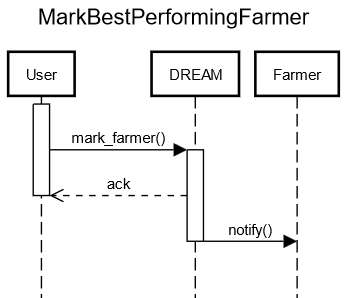
\includegraphics[scale=0.5]{sequence_diagrams/MarkBestPerformingFarmer.png}
    \caption{Sequence diagram for the MarkBestPerformingFarmer use case}
\end{figure}
OBS.: the use case MarkWorstPerformingFarmer is exactly the same.
\newpage

%%%%%%%%%%%%%%%%%%%%%%%%%%%%TABLE 18%%%%%%%%%%%%%%%%%%%%%%%

\centering
\begin{longtable}{|p{3.5cm}|m{8cm}|}
\caption{Use case 17: UnmarkBestPerformingFarmer}
 \label{uc17}
 \hline
 \multicolumn{2}{|c|}{\cellcolor{white}\emph{USE CASE 17}} \\
  % do not write anything here
 \endfirsthead
 % do not write anything here
 \endhead
 % do not write anything here
 \endfoot
 % do not write anything here
 \endlastfoot
 \hline
 Name & UnmarkBestPerformingFarmer\\
 \hline
 Actor & User (Policy Maker or Agronomist), Farmer\\
 \hline
 Entry condition & The user is logged in the system and is visualizing a list of farmers ranked according to some criteria he/she has chosen. He/she wants to unmark a best-performing farmer.\\
 \hline
 Event flow & \begin{enumerate}
    \item The user clicks on the "Unmark" button related to a best-performing farmer.
    \item \verb|DREAM| shows the user a confirm of having unmarked the farmer.
    \item \verb|DREAM| sends the farmer a notification about the fact he/she has been unmarked.
 \end{enumerate}\\
 \hline
 Exit condition &  When policy makers and agronomists of the area of the farmer will visualize the farmer in a list in the "Farms" section, he/she will no more be shown as best-performing.
 Other farmers are not able anymore to send questions to the farmer - the My Replies section in the homepage of the farmer stays there, to display past replies.\\
 \hline
 Exceptions & -\\
 \hline
 Special requirements &\begin{itemize}
     \item After the policy maker clicks on the "Unmark" button, the confirm should be shown and the notification should be sent in less than 10 seconds.
 \end{itemize}\\
 \hline
\end{longtable}

\begin{figure}[H]
    \centering
	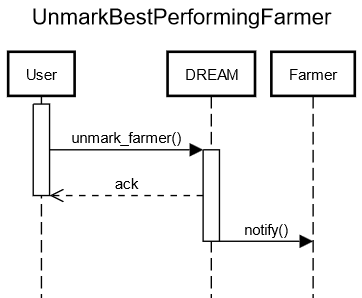
\includegraphics[scale=0.5]{sequence_diagrams/UnmarkBestPerformingFarmer.png}
    \caption{Sequence diagram for the UnmarkBestPerformingFarmer use case.}
\end{figure}

OBS.: the use case UnmarkWorstPerformingFarmer is exactly the same.
\newpage

%%%%%%%%%%%%%%%%%%%%%%%%%%%%TABLE 19%%%%%%%%%%%%%%%%%%%%%%%

\centering
\begin{longtable}{|p{3.5cm}|m{8cm}|}
\caption{Use case 18: AnalyzeImpactOfInitiative}
 \label{uc18}
 \hline
 \multicolumn{2}{|c|}{\cellcolor{white}\emph{USE CASE 18}} \\
  % do not write anything here
 \endfirsthead
 % do not write anything here
 \endhead
 % do not write anything here
 \endfoot
 % do not write anything here
 \endlastfoot
 \hline
 Name & AnalyzeImpactOfInitiative\\
 \hline
 Actor & Policy Maker, TSDPSSystem\\
 \hline
 Entry condition & The policy maker is logged in the system and wants to analyze the impact of an initiative - i.e., visit to the farm or reply to a question - on the production of a certain farmer.\\
 \hline
 Event flow & \begin{enumerate}
    \item From the homepage, the policy maker accesses the "Initiatives Analysis" section.
    \item \verb|DREAM| shows a list of initiatives - either visit to a farm or reply to a question of a farmer -, and some input fields to filter the initiatives according to the type (visit or reply), the date, the area of the farmer, the agronomist or best-performing farmer involved.
    \item The policy maker selects one of the initiatives.
    \item \verb|DREAM| fetches weather reports data from the TSDPS system
 \end{enumerate}\\
 \hline
 Exit condition &  \verb|DREAM| shows details about the initiative and indicators comparing the farmer production data 30 days before and 30 days after the initiative, such as percent difference between the production volume or percent difference between the amount harvested over the amount seeded for each crop, resilience to adverse meteorological events. Moreover, there are two input fields to change the time scope for computing the indicators.\\
 \hline
 Exceptions & -\\
 \hline
 Special requirements &\begin{itemize}
     \item After the policy maker selects the initiative, the result should be shown in less than 10 seconds.
 \end{itemize}\\
 \hline
\end{longtable}

\begin{figure}[H]
    \centering
	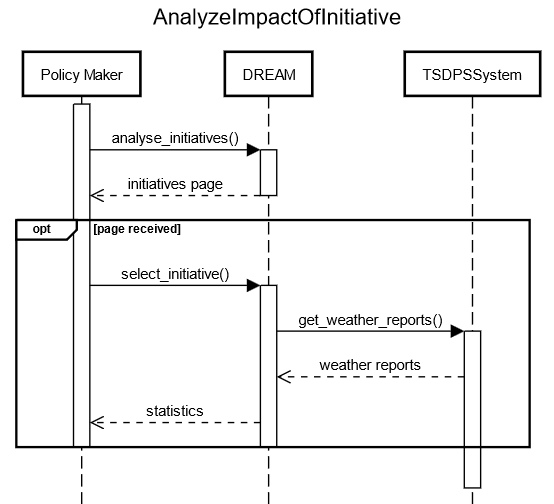
\includegraphics[scale=0.5]{sequence_diagrams/AnalyzeImpactOfInitiative.png}
    \caption{Sequence diagram for the AnalyzeImpactOfInitiative use case.}
\end{figure}
\newpage
%%%%%%%%%%%%%%%%%%%TABLE 19%%%%%%%%%%%%%%%%

\centering
\begin{longtable}{|p{3.5cm}|m{8cm}|}
\caption{Use case 19: VisualizeWeatherForecasts}
 \label{uc19}
 \hline
 \multicolumn{2}{|c|}{\cellcolor{white}\emph{USE CASE 19}} \\
  % do not write anything here
 \endfirsthead
 % do not write anything here
 \endhead
 % do not write anything here
 \endfoot
 % do not write anything here
 \endlastfoot
 \hline
 Name & VisualizeWeatherForecasts\\
 \hline
 Actor & User (either Farmer or Agronomist), TSDPSSystem \\
 \hline
 Entry condition & The user is logged in the system and wants to visualize the weather forecast for the area of his/her farm (if he/she is a farmer) or the area he/she is assigned to (if he/she is an agronomist).\\
 \hline
 Event flow & \begin{enumerate}
    \item From the homepage, the user accesses the WeatherForecasts section.
    \item \verb|DREAM| shows an input field for inserting the date for which the forecasts should be shown, and if the user is an agronomist, the list of the mandals in the area he/she is responsible of.
    \item If the user is an agronomist, he/she selects the mandal in his area for which he/she wants to visualize the forecasts. 
    \item The user selects the date for which he/she wants to visualize the forecasts.
    \item \verb|DREAM| fetches from the TSDPSSystem the weather forecast for the selected date and for the chosen mandal (if the user is an agronomist) or for the mandal of the farmer's farm (if the user is a farmer) (view UC23 for more details).
 \end{enumerate}\\
 \hline
 Exit condition & \verb|DREAM| shows a table containing the weather forecasts for the chosen date and mandal. \\
 \hline
 Exceptions & \begin{itemize}
     \item If the Telangana government website is currently unreachable, an error message is shown to the user.
     \item If no weather data is available for the chosen date, an error message is shown to the user.
 \end{itemize}\\
 \hline
 Special requirements &\begin{itemize}
     \item The weather forecasts should be shown in less than 10 seconds.
 \end{itemize}\\
 \hline
\end{longtable}

\begin{figure}[H]
    \centering
	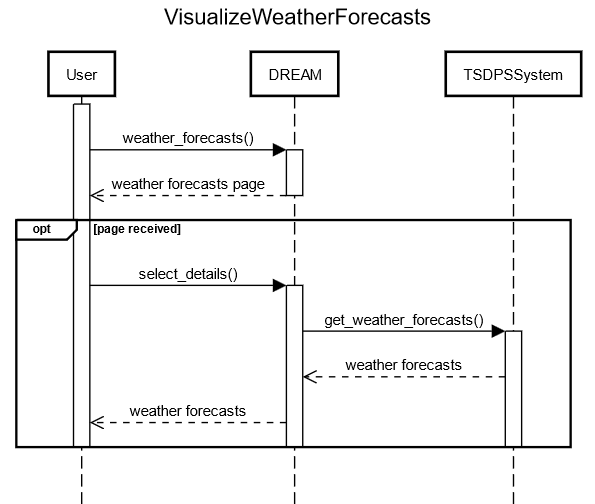
\includegraphics[scale=0.5]{sequence_diagrams/VisualizeWeatherForecasts.png}
    \caption{Sequence diagram for the VisualizeWeatherForecasts use case.}
\end{figure}
\newpage

%%%%%%%%%%%%%%%%%%%%%%%%%%%%TABLE 22%%%%%%%%%%%%%%%%%%%%%%%

\centering
\begin{longtable}{|p{3.5cm}|m{8cm}|}
\caption{Use case 20: VisualizeFarmerSuggestions}
 \label{uc20}
 \hline
 \multicolumn{2}{|c|}{\cellcolor{white}\emph{USE CASE 20}} \\
  % do not write anything here
 \endfirsthead
 % do not write anything here
 \endhead
 % do not write anything here
 \endfoot
 % do not write anything here
 \endlastfoot
 \hline
 Name & VisualizeFarmerSuggestions\\
 \hline
 Actor & Farmer, TSDPSSystem\\
 \hline
 Entry condition & The farmer is logged into the system and wants to check if there are any suggestions for him/her.\\
 \hline
 Event flow & \begin{enumerate}
    \item From the homepage, the farmer accesses the Suggestions section;
    \item \verb|DREAM| retrieves weather forecasts and reports necessary for computing the suggestions from the TSDPSSystem (view UC23 for more details).
    \item \verb|DREAM| shows a list of suggestions for the farmer.
 \end{enumerate}\\
 \hline
 Exit condition & The farmer views the list of suggestions.\\
 \hline
 Exceptions & \begin{itemize}
     \item If there are no suggestions for the farmer, a message is shown.
 \end{itemize}\\
 \hline
 Special requirements & The farmer should be shown the suggestions in less than 20 seconds.\\
 \hline
\end{longtable}
\begin{figure}[H]
    \centering
	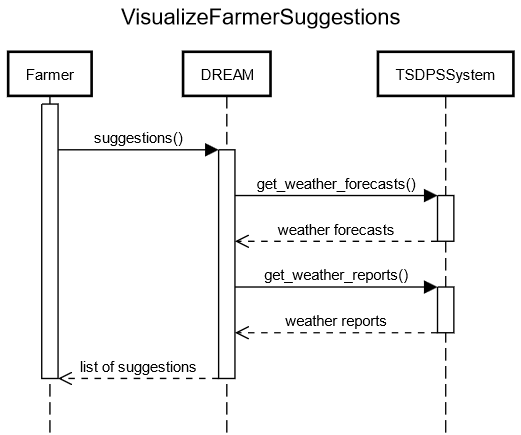
\includegraphics[scale=0.5]{sequence_diagrams/VisualizeFarmerSuggestions.png}
    \caption{Sequence diagram for the VisualizeFarmerSuggestions use case.}
\end{figure}
\newpage

%%%%%%%%%%%%%%%%%%%%%%%%%%%%TABLE 23%%%%%%%%%%%%%%%%%%%%%%%

\centering
\begin{longtable}{|p{3.5cm}|m{8cm}|}
\caption{Use case 21: GetWeatherForecasts}
 \label{uc21}
 \hline
 \multicolumn{2}{|c|}{\cellcolor{white}\emph{USE CASE 21}} \\
  % do not write anything here
 \endfirsthead
 % do not write anything here
 \endhead
 % do not write anything here
 \endfoot
 % do not write anything here
 \endlastfoot
 \hline
 Name & GetWeatherForecasts\\
 \hline
 Actor & TSDPSSystem\\
 \hline
 Entry condition & Either (a) a user requests weather data; or (b) \verb|DREAM| needs to access weather forecasts for computing suggestions for some farmer.\\
 \hline
 Event flow & \begin{enumerate}
    \item \verb|DREAM| requests the TSDPSSystem the needed weather forecast 
    \item The TSDPSSystem replies with the required weather forecasts 
 \end{enumerate}\\
 \hline
 Exit condition & The weather forecast are available to the \verb|DREAM| system.\\
 \hline
 Exceptions & \begin{itemize}
     \item If the TSDPSSystem is currently unreachable, the process is aborted and an error is returned to the user.
 \end{itemize}\\
 \hline
 Special requirements & - \\
 \hline
\end{longtable}
\begin{figure}[H]
    \centering
	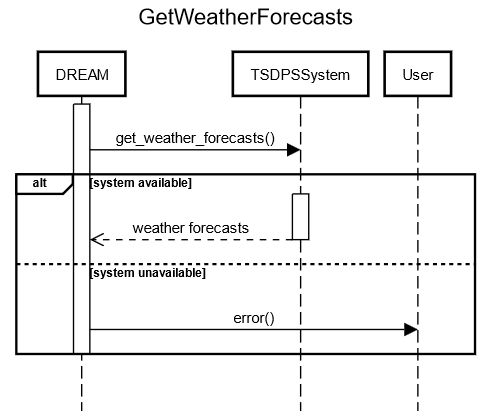
\includegraphics[scale=0.5]{sequence_diagrams/GetWeatherForecasts.png}
    \caption{Sequence diagram for the GetWeatherForecasts use case.}
\end{figure}
The interaction is analogous for retrieving weather reports.
\newpage
%%%%%%%%%%%TABLE 21%%%%%%%%%%%%%%%%%%%%%%%%%%%%%%%%%%%%%%%%

\centering
\begin{longtable}{|p{3.5cm}|m{8cm}|}
\caption{Use case 22: RequestToExpert}
 \label{uc22}
 \hline
 \multicolumn{2}{|c|}{\cellcolor{white}\emph{USE CASE 22}} \\
  % do not write anything here
 \endfirsthead
 % do not write anything here
 \endhead
 % do not write anything here
 \endfoot
 % do not write anything here
 \endlastfoot
 \hline
 Name & RequestToExpert\\
 \hline
 Actor & Farmer, Expert (either an Agronomist or a best-performing Farmer)\\
 \hline
 Entry condition & The Farmer is logged in the \verb|DREAM| system and wants to ask a question to an Agronomist or to another Farmer.\\
 \hline
 Event flow & \begin{enumerate}
    \item From the homepage, the Farmer enters the "My Requests" section.
    \item The Farmer clicks on the "New Request" button and selects the type of expert he wants to ask his question.
    \item \verb|DREAM| responds showing the list of experts of that kind available.
    \item The Farmer selects from the list the expert to contact, then inserts in a form all the data of the request (title, description) and sends the request.
    \item \verb|DREAM| forwards the request to the chosen expert – that is, it inserts the request in the list of the new requests issued to the expert.
    \item \verb|DREAM| shows a confirmation of having sent the request, containing the name of the expert, the title and the description of the request.
 \end{enumerate}\\
 \hline
 Exit condition & The request is present in the list in the "My Requests" section of the Farmer view, shown as a closed request, and selecting it from the list the Farmer can see the name of the Expert, the timestamp, title and text of the request, the timestamp and text of the reply, and the feedback message.\\
 \hline
 Exceptions & \begin{itemize}
    \item If the device of the Expert is not connected to the Internet when he should receive the request, then \verb|DREAM| shows the details of the request and a message saying that it will be sent as soon as the device will be connected to the Internet. When the disconnected device reconnects, the message is sent.
 \end{itemize}\\
 \hline
 Special requirements & \begin{itemize}
     \item The messages between the Farmer and the Expert are delivered in less than one minute.
 \end{itemize}\\
 \hline
\end{longtable}

\begin{figure}[H]
    \centering
    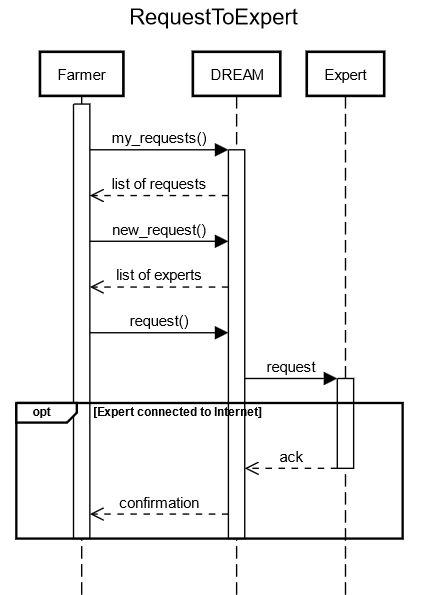
\includegraphics[scale=0.75]{sequence_diagrams/RequestToExpert.png}
    \caption{Sequence diagram for the RequestToExpert use case.}
\end{figure}
\newpage
%%%%%%%%%%%TABLE 22%%%%%%%%%%%%%%%%%%%%%%%%%%%%%%%%%%%%%%%%

\centering
\begin{longtable}{|p{3.5cm}|m{8cm}|}
\caption{Use case 23: ExpertResponse}
 \label{uc23}
 \hline
 \multicolumn{2}{|c|}{\cellcolor{white}\emph{USE CASE 23}} \\
  % do not write anything here
 \endfirsthead
 % do not write anything here
 \endhead
 % do not write anything here
 \endfoot
 % do not write anything here
 \endlastfoot
 \hline
 Name & ExpertResponse\\
 \hline
 Actor & Farmer, Expert (either an Agronomist or a best-performing Farmer)\\
 \hline
 Entry condition & The Expert is logged in the \verb|DREAM| system.\\
 \hline
 Event flow & \begin{enumerate}
    \item From the homepage, the Expert enters the "My Responses" section.
    \item The Expert selects one request from the list of non-answered requests.
    \item \verb|DREAM| shows the name of the Farmer, the timestamp, the title and the description of the request, and a form to insert the reply.
    \item The Experts fills the form with the response and clicks on the "Send Reply" button.
    \item \verb|DREAM| forwards the reply to the Farmer – that is, it associates the reply to the request of the Farmer.
    \item \verb|DREAM| shows a confirmation of having sent the reply, containing the name of the Farmer, the title and the text of the request, and the text of the reply.
 \end{enumerate}\\
 \hline
 Exit condition & The request is present in the list in the "My Responses" section of the Expert, shown as a closed request.\\
 \hline
 Exceptions & \begin{itemize}
    \item If the device of the Farmer is not connected to Internet when the Expert sends the response, then \verb|DREAM| shows a message saying that it will be sent as soon as the device will be connected to Internet. When the disconnected device reconnects, the message is sent.
 \end{itemize}\\
 \hline
 Special requirements & \begin{itemize}
     \item The messages between the Farmer and the Expert are delivered in less than one minute.
 \end{itemize}\\
 \hline
\end{longtable}

\begin{figure}[H]
    \centering
    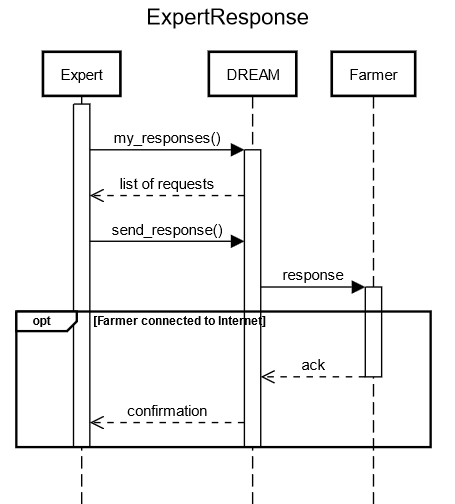
\includegraphics[scale=0.75]{sequence_diagrams/ExpertResponse.png}
    \caption{Sequence diagram for the ExpertResponse use case.}
\end{figure}
\newpage
%%%%%%%%%%%TABLE 23%%%%%%%%%%%%%%%%%%%%%%%%%%%%%%%%%%%%%%%%

\centering
\begin{longtable}{|p{3.5cm}|m{8cm}|}
\caption{Use case 24: VisualiseResponse}
 \label{uc24}
 \hline
 \multicolumn{2}{|c|}{\cellcolor{white}\emph{USE CASE 24}} \\
  % do not write anything here
 \endfirsthead
 % do not write anything here
 \endhead
 % do not write anything here
 \endfoot
 % do not write anything here
 \endlastfoot
 \hline
 Name & VisualiseResponse\\
 \hline
 Actor & Farmer\\
 \hline
 Entry condition & The Farmer is logged in the \verb|DREAM| system.\\
 \hline
 Event flow & \begin{enumerate}
    \item From the homepage, the Farmer enters the "My Requests" section.
    \item \verb|DREAM| shows a list of the requests issued by the Farmer, where the ones which the response hasn't been read yet are highlighted.
    \item The Farmer selects the request the Expert has replied to.
    \item \verb|DREAM| shows the timestamp, title and text of the request, the name of the Expert who has replied, and the timestamp and text of the reply, and a text input to provide a feedback to the Expert.
    \item The Farmer writes down his feedback to the Expert.
    \item The Farmer clicks on the "Send" button.
    \item \verb|DREAM| sends the feedback to the expert – that is, it associates the feedback to the request-reply thread.

 \end{enumerate}\\
 \hline
 Exit condition & The farmer visualises the response of the expert and the expert has received a feedback from the farmer.\\
 \hline
 Exceptions & -
 \hline
 Special requirements & -
 \hline
\end{longtable}

\begin{figure}[H]
    \centering
    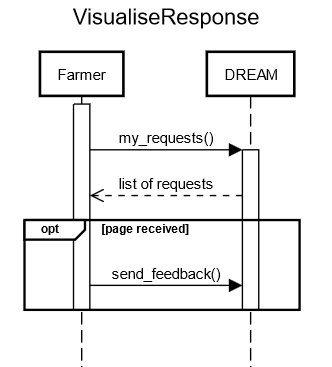
\includegraphics[scale=0.75]{sequence_diagrams/VisualiseResponse.png}
    \caption{Sequence diagram for the VisualiseResponse use case.}
\end{figure}
\newpage

%%%%%%%%%%%%%%%%%%%%%%%%%%%%TABLE 24%%%%%%%%%%%%%%%%%%%%%%%

\centering
\begin{longtable}{|p{3.5cm}|m{8cm}|}
\caption{Use case 25: CreateFarmersForumThread}
 \label{uc25}
 \hline
 \multicolumn{2}{|c|}{\cellcolor{white}\emph{USE CASE 25}} \\
  % do not write anything here
 \endfirsthead
 % do not write anything here
 \endhead
 % do not write anything here
 \endfoot
 % do not write anything here
 \endlastfoot
 \hline
 Name & CreateFarmersForumThread\\
 \hline
 Actor & Farmer\\
 \hline
 Entry condition & The Farmer is logged in the \verb|DREAM| system, and visualizes the home page.\\
 \hline
 Event flow & \begin{enumerate}
    \item From the homepage, the Farmer enters the Forum section.
    \item \verb|DREAM| replies showing a list of the already present discussion threads and a "New Thread" button.
    \item The Farmer clicks on the "New Thread" button.
    \item \verb|DREAM| shows a text input area to insert the name of the "New Thread",  and a "Create" button.
    \item The Farmer inserts the title of the discussion thread.
    \item The Farmer clicks on the "New Thread" button.

 \end{enumerate}\\
 \hline
 Exit condition & A new thread of discussion has been created, which can be seen by all farmers when entering the "Forum" section.
The Farmer visualizes the list of messages in the thread – which is empty – together with a "New Post" button.\\
 \hline
 Exceptions & \begin{itemize}
     \item If the title inserted by the Farmer is not valid (empty or already present), an error message is shown and the new thread is not created.
 \end{itemize}\\
 \hline
\end{longtable}
\begin{figure}[H]
    \centering
	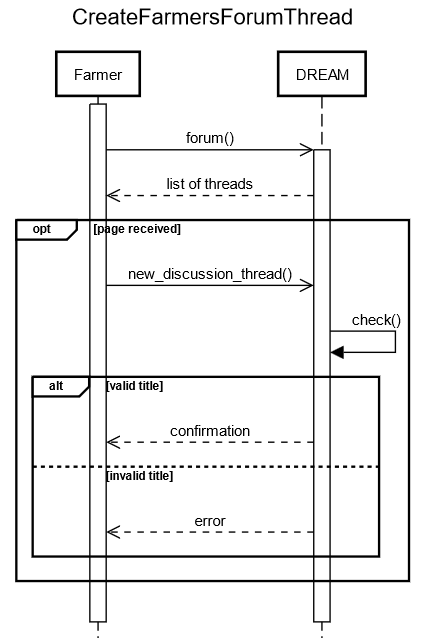
\includegraphics[scale=0.5]{sequence_diagrams/CreateFarmersForumThread.png}
    \caption{Sequence diagram for the CreateFarmersForumThread use case.}
\end{figure}
\newpage

%%%%%%%%%%%%%%%%%%%%%%%%%%%%TABLE 25%%%%%%%%%%%%%%%%%%%%%%%

\centering
\begin{longtable}{|p{3.5cm}|m{8cm}|}
\caption{Use case 26: WritePostOnFarmersForum}
 \label{uc26}
 \hline
 \multicolumn{2}{|c|}{\cellcolor{white}\emph{USE CASE 26}} \\
  % do not write anything here
 \endfirsthead
 % do not write anything here
 \endhead
 % do not write anything here
 \endfoot
 % do not write anything here
 \endlastfoot
 \hline
 Name & WritePostOnFarmersForum\\
 \hline
 Actor & Farmer\\
 \hline
 Entry condition & The Farmer is logged in the \verb|DREAM| system, and visualizes the home page.\\
 \hline
 Event flow & \begin{enumerate}
    \item From the homepage, the Farmer enters the Forum section.
    \item \verb|DREAM| replies showing a list of the already present discussion threads and a "New Thread" button.
    \item The Farmer clicks on one of the already present discussion threads.
    \item \verb|DREAM| shows a list of the posts in the forum, an input text field and a "New Post" button.
    \item The Farmer inserts the text of the post.
    \item The Farmer clicks on the "New Post" button.
 \end{enumerate}\\
 \hline
 Exit condition & \verb|DREAM| shows a confirmation of having created the new post, and the post is shown together with the others in the list.\\
 \hline
 Exceptions & \begin{itemize}
     \item If the text of the post is empty, \verb|DREAM| shows an error message and doesn't create any new post.
 \end{itemize}\\
 \hline
\end{longtable}
\begin{figure}[H]
    \centering
	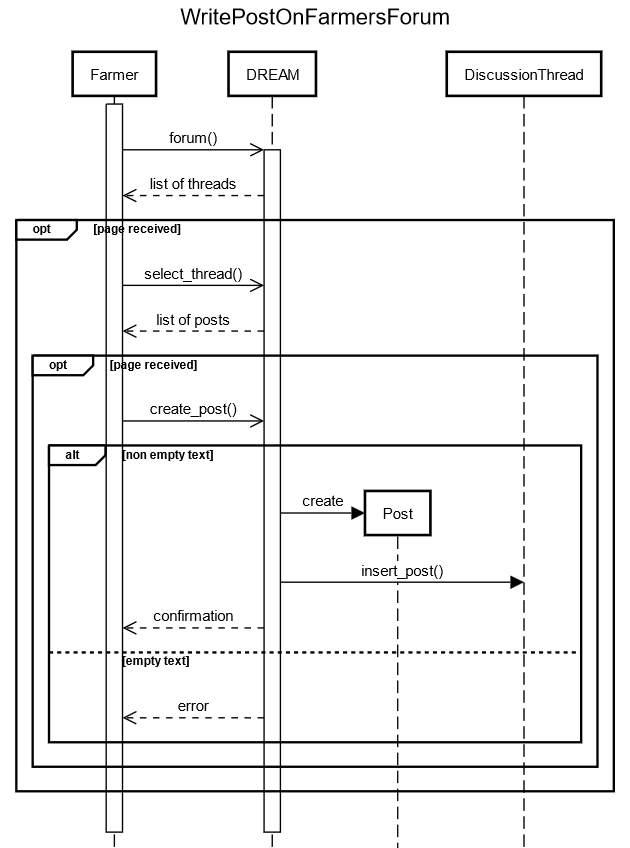
\includegraphics[scale=0.5]{sequence_diagrams/WritePostOnFarmersForum.png}
    \caption{Sequence diagram for the WritePostOnFarmersForum use case.}
\end{figure}
\newpage
\raggedright



\subsubsection{Mapping between use cases and requirements}
This section shows how the \verb|DREAM| system implements requirements by mapping them to use cases.

\begin{longtable}[c]{|m{3,5cm}|m{8cm}|}
 %%%%%%%%%%%%%%%%%%%%%%%%%%%%%%%%%%
\caption{Mapping between use cases and requirements.}
 \label{Mapping UC - R}
%%%%%%%%%%%%%%%%%%%%%%%%%%%%%%%%%
  \hline
  UC1: RegisterFarmer &
\begin{itemize}
    \item R5: \verb|DREAM| shall allow farmers to insert the location and the area of their plot of land;
\end{itemize}\\
\hline
 UC2: RegisterAgronomist &
\begin{itemize}
    \item R29: \verb|DREAM| shall allow agronomists to insert the area they are responsible of;
\end{itemize}\\
\hline
UC3: LogIn & 
\begin{itemize}
    \item R48: \verb|DREAM| shall allow users to log in the system by using an email and a password;
\end{itemize}\\
\hline
UC4: ViewProductionData & 
\begin{itemize}
    \item R49: \verb|DREAM| shall allow farmers to visualize data inserted by them about their production;
\end{itemize}\\
\hline
UC5: InsertProductionData & 
\begin{itemize}
        \item R6: \verb|DREAM| shall allow farmers to insert the type of products they grow in a certain area of their farms;

        \item R7: \verb|DREAM| shall allow farmers to insert data about their sowing activity;
    
        \item R8: \verb|DREAM| shall allow farmers to insert data about their planting activity;
        
        \item R9: \verb|DREAM| shall allow farmers to insert data about their harvesting activity;
        
        \item R10: \verb|DREAM| shall allow farmers to insert data about the irrigation of their plantations;
    \end{itemize}\\
\hline
  \item UC6: InsertProblems & 
    \begin{itemize}
        \item R11: \verb|DREAM| shall allow farmers to insert descriptions of problems they face;
    
  \item R12: \verb|DREAM| shall allow farmers to request a visit of an agronomist when inserting a problem;

  \item R13: When a farmer requests a visit of an agronomist, \verb|DREAM| inserts the visit to the farmer into the daily plan of an agronomist assigned to the area of the farmer;

  \item R14: When a farmer requests a visit of an agronomist, if no agronomist is available in the area of the farmer during the seven days after the request (excluding the day when the request is made), \verb|DREAM| notifies the farmer about this situation.
    \end{itemize}\\
\hline
UC7: AcceptDailyPlan & 
\begin{itemize}
    \item R39: \verb|DREAM| enforces that every farmer is assigned a visit in the daily plan of an agronomist at least twice a year;

    \item R40: \verb|DREAM| enforces that no agronomist in a certain area is assigned more than twice of the visits than an agronomist of the same area;

    \item R41: \verb|DREAM| enforces that the daily plan of agronomists includes more visits to worst-performing farmers than to other ones;

    \item R42: \verb|DREAM| allows agronomists to accept or modify -i.e.: remove, add or move a visit - the automatically generated daily plan;

    \item R45: \verb|DREAM| is able to notify farmers involved by a visit of an agronomist;
\end{itemize}\\ \hline
\hline
UC8: ViewDetailsOfFarmToVisit & 
\begin{itemize}
    \item R46: \verb|DREAM| allows agronomists to visualize data about farmers to visit - such as name, surname and location of the farm -  and their production since their last visit to the farm;
\end{itemize}\\
\hline
UC9: MoveVisitInDailyPlan & 
\begin{itemize}
    \item R39: \verb|DREAM| enforces that every farmer is assigned a visit in the daily plan of an agronomist at least twice a year;

    \item R40: \verb|DREAM| enforces that no agronomist in a certain area is assigned more than twice of the visits than an agronomist of the same area;

    \item R41: \verb|DREAM| enforces that the daily plan of agronomists includes more visits to worst-performing farmers than to other ones;

    \item R42: \verb|DREAM| allows agronomists to accept or modify -i.e.: remove, add or move a visit - the automatically generated daily plan;

    \item R45: \verb|DREAM| is able to notify farmers involved by a visit of an agronomist;
\end{itemize}\\ \hline
\hline
UC10: DeleteVisitFromDailyPlan & 
\begin{itemize}
    \item R39: \verb|DREAM| enforces that every farmer is assigned a visit in the daily plan of an agronomist at least twice a year;

    \item R40: \verb|DREAM| enforces that no agronomist in a certain area is assigned more than twice of the visits than an agronomist of the same area;

    \item R41: \verb|DREAM| enforces that the daily plan of agronomists includes more visits to worst-performing farmers than to other ones;

    \item R42: \verb|DREAM| allows agronomists to accept or modify -i.e.: remove, add or move a visit - the automatically generated daily plan;

    \item R45: \verb|DREAM| is able to notify farmers involved by a visit of an agronomist;
\end{itemize}\\ \hline
\hline
UC11: AddVisitToDailyPlan & 
\begin{itemize}
    \item R39: \verb|DREAM| enforces that every farmer is assigned a visit in the daily plan of an agronomist at least twice a year;

    \item R40: \verb|DREAM| enforces that no agronomist in a certain area is assigned more than twice of the visits than an agronomist of the same area;

    \item R41: \verb|DREAM| enforces that the daily plan of agronomists includes more visits to worst-performing farmers than to other ones;

    \item R42: \verb|DREAM| allows agronomists to accept or modify -i.e.: remove, add or move a visit - the automatically generated daily plan;

    \item R45: \verb|DREAM| is able to notify farmers involved by a visit of an agronomist;
\end{itemize}\\ \hline
\hline
UC12: ConfirmDailyPlan & 
\begin{itemize}
    \item R4: \verb|DREAM| shall allow agronomists to insert feedback about the farmers they visited;
    
    \item R43: \verb|DREAM| allows agronomists to confirm a daily plan at the end of the working day; 

    \item R44: \verb|DREAM| allows agronomists to specify deviations -i.e.: remove, add or move a visit- from a daily plan at the end of the working day; 
\end{itemize}\\
\hline
UC13: GetSoilSensorsData & 
\begin{itemize}
    \item R1: \verb|DREAM| collects soil moisture data from the soil moisture sensors;
\end{itemize} \\ \hline
\hline
UC14: GetWaterIrrigationSystemData & 
\begin{itemize}
    \item R3: \verb|DREAM| collects watering data from the water irrigation system;
\end{itemize} \\ \hline
\hline
UC15: VisualizeBestAndWorstFarmers & 
\begin{itemize}
    \item R15: \verb|DREAM| can use different criteria (namely, productivity in terms of harvested quantity over sowed quantity, productivity in presence of adverse meteorological events, productivity in presence of drought, and so on) and/or combinations of them to rank farmers;
    
    \item R16: \verb|DREAM| shall allow policy makers and agronomists to choose the criteria to use for ranking farmers and the associated weights (for combinations of them);
    
    \item R17: \verb|DREAM| shall allow policy makers and agronomists to choose the time period and the area to consider for ranking the farmers;
\end{itemize} \\
\hline
UC16: MarkBestPerformingFarmer & 
\begin{itemize}
    \item R18: \verb|DREAM| allows policy makers and agronomists to mark/unmark a farmer as best-performing
or worst-performing;
\end{itemize}\\
\hline
UC17: UnmarkBestPerformingFarmer & 
\begin{itemize}
    \item R18: \verb|DREAM| allows policy makers and agronomists to mark/unmark a farmer as best-performing
or worst-performing;
\end{itemize}\\
\hline
UC18: AnalyzeImpactOfInitiative & 
\begin{itemize}
    \item R19:
\verb|DREAM| can compare different time periods of a farmer work according to
various production criteria (e.g. production volume, fertilizers adopted,
fraction of harvested plants over sowed ones, etc);
\item
R20:
\verb|DREAM| can compare different time periods of a farmer work with respect
to environmental factors (e.g. weather reports data, soil moisture, ...);
\item
R21:
\verb|DREAM| allows policy makers to choose an initiative taken by an
agronomist or a farmer to help a farmer - i.e., visit to the farm or reply
to a question - and two time periods of the farmer to compare the two
time periods;
\item R22:
\verb|DREAM| can show the impact of a certain initiative taken by an agronomist
or a farmer to help a farmer - i.e., visit to the farm or reply to a question
- during a certain time period.
\end{itemize}\\
\hline
UC19: VisualizeWeatherForecasts &
\begin{itemize}
    \item R27: \verb|DREAM| is able to connect to the Telangana government website to fetch forecasts for the chosen date;

    \item R28: \verb|DREAM| can show weather forecast data for a certain location and date;

    \item R30: \verb|DREAM| shall allow agronomists to choose the date of the weather forecasts to visualize; 
\end{itemize} \\ 
\hline
UC20: VisualizeFarmerSuggestions & 
\begin{itemize}
    \item R23: \verb|DREAM| is able to find correlations among environmental factors, fertilisers adopted and crops planted with the volume of production of the farmers;
 
    \item R24: \verb|DREAM| is able to send suggestions to farmers about fertilizers to use;
    
    \item R25: \verb|DREAM| is able to send suggestions to farmers about crops to plant; 
\end{itemize} \\ 
\hline
UC21: GetWeatherForecasts & 
\begin{itemize}
    \item R27: \verb|DREAM| is able to connect to the Telangana government website to fetch forecasts for the chosen date;
\end{itemize} \\ \hline
\hline
UC22: RequestToExpert & 
\begin{itemize}
    \item R31: \verb|DREAM| allows farmers to choose the (best-performing) farmer or agronomist (assigned to his area) who to issue a request;
  
    \item R32: \verb|DREAM| allows the farmers to send a request to a best-performing farmer or agronomist.
    


    
\end{itemize} \\ \hline
\hline
UC23: ExpertResponse & 
\begin{itemize}
        \item R33: \verb|DREAM| notifies (best-performing) farmers and agronomists of the requests of help from other farmers;

    \item R34: \verb|DREAM| allows best-performing farmers and agronomists to insert a message of response to the farmers who have made a request for help to them.
\end{itemize}\\
\hline
UC24: VisualizeResponse & 
\begin{itemize}
    \item R35: \verb|DREAM| sends the response to the farmer who issued the corresponding request.
\end{itemize}\\
\hline
UC25: CreateFarmersForumThread & 
\begin{itemize}
    \item R36: \verb|DREAM| allows farmers to initiate a new thread in the forum.
\end{itemize}
\hline
UC26: WritePostOnFarmersForum & 
\begin{itemize}
    \item R37: \verb|DREAM| allows the farmers to add a post to a thread in the forum;
\end{itemize} \\ \hline
\end{longtable}


\newpage
\raggedright
\subsection{Performance Requirements}
This section is dedicated to “specify both the static and the dynamic numerical requirements placed on the software or on human interaction with the software as a whole”\footnote{IEEE 29148-2018 Requirements engineering, section 9.6.14}.
Static numerical requirements:
\begin{itemize}
\item according to the estimates\footnote{professor Jayashankar Telangana state agricultural university}, Telangana has a population of 36 millions of people and a total number of farm holdings equal to 55.54 lakhs, namely more or less 5 555 400 people in Telangana are farmers; assuming that all of them are potential users of \verb|DREAM|, it must support at least 5.7 million non-simultaneously connected terminals, since also the agronomists and policy makers shall be allowed to access the system;
\item given the huge number of (possible) users and the purpose of the system, \verb|DREAM| must be able to support at least 10\% of the total number of users simultaneously; this requirement is more important than speed performances;
\item all the weather reports and forecasts are not directly stored on \verb|DREAM|; nevertheless, \verb|DREAM| must store all the sensors and water irrigation system data as well as the users data and the forums data. 
We can assume that the system stores 1KB of personal information for each user:
\[ usersData = 5.7 * 10^6 users * 1 KB \approx 5.7 GB \]
Assuming an average of 1000 posts a day, the data required for 1 year is (assumption: 1KB for each post, no images allowed):
\[forumData = 1 KB * 1000 posts/day * 365 days/year \approx 365 MB \]
Plus 32 bytes for each sensor measurement (16 bytes to recognize the sensor, 8 bytes for the timestamp and 8 bytes for the soil moisture value; we estimate 10 000 humidity sensors in Telangana whose data is retrieved 3 times a day):
\[sensorsData = 32 B * 10 000 sensors * 3 measurements/day * 365 days/year \approx 350 MB \]
Plus 32B additional bytes for each farmer because of the water irrigation system:
\[waterIrrigationSystemData = 32 B * 12 measurements/year * 5.5 * 10^6 farmers \approx 2 GB \]
Plus 1KB for each production report stored in \verb|DREAM| (assuming that each farmer uploads the production data once for each month):
\[productionData = 1 KB * 12 reports/year * 5.5 * 10^6 farmers \approx 66 GB \]
Plus some additional data for the daily plans, that we can neglect because of the small number of agronomists with regards to the number of farmers.\\
This means that the amount of information to be effectively stored must be in the rank of:
\[totalData = \sum_{i=1}^{5} data[i] \approx 74 GB \]
In this calculation is not considered all the space required to perform analysis over the stored data and the data accessed over the Telangana's government website (namely, weather reports and forecasts). Therefore, we can assume that a database of $100 GB$ can suffice for the first year.
\end{itemize}
Dynamic numerical requirements:
\begin{itemize}
\item all the transactions must be processed in less than 3 seconds (as said before, \verb|DREAM| does not require strict temporal requirements);
\item the number of transactions the system has to process during peak workload conditions is in the order of $10^4$.
\end{itemize}

\subsection{Design Constraints}
In this section we “specify constraints on the system design imposed by external standards, regulatory requirements or project limitations”\footnote{IEEE 29148-2018 Requirements engineering, section 9.6.16}.
\subsubsection{Standard compliance}
\verb|DREAM| stores personal data of the users, like name, surname, job, location of the farm (if he is a farmer) … . Therefore, this data must be treated according to the privacy regulations in India.
\subsubsection{Hardware limitation}
Since \verb|DREAM| is a webapp, every device with a browser recent enough can be used to access the system. \verb|DREAM| does not impose any constraint on the sensors and the water irrigation system, as long as the central hub uses a standardized protocol for communication.
\subsubsection{Any other constraint}
No any other specific constraint is required.
\subsection{Software System Attributes}
In this section a list of required attributes of the system is provided.
\subsubsection{Reliability}
\verb|DREAM| is not a critical system, therefore some limited failures cannot create big problems. For example, an error when accessing the Telangana’s website or a failure during the generation of the daily plan can be easily solved just by re-starting the process.
\subsubsection{Availability}
The system is not critical, as already said, therefore some periods of inactivity are allowed. Because all the tasks it performs are not critical, small periods of inactivity do not create many problems. For instance, when a farmer needs to ask for help, he could make the request even the following day. Another example is the access to the humidity sensors: data of today could be accessed even tomorrow since they are stored in Telangana’s website as well. A final example is about the proposal of a schedule plan; agronomists can wait some time before retrieving it. 
We can impose that \verb|DREAM| must not be unavailable for more than 1 day per month.
\subsubsection{Security}
The only information that needs to be protected is the personal data of the users. Therefore, \verb|DREAM| has to assure data privacy. This can be done by ensuring that all connections are established securely via HTTPS.
\subsubsection{Maintainability}
The system must be designed in order to facilitate maintainability. Every functionality implemented must be well documented. The system must be decomposed in a certain number of modules to limit the complexity and to make the development process more efficient. The main goal is that each module is coherent and can be (internally) modified without affecting other modules and without changing its interface.
\subsubsection{Portability}
Since \verb|DREAM| is a webapp, it does not have strict requirements on the underlying operating system or hardware used. The website will be developed using an interpreted language with a widely available interpreter. Furthermore, \verb|DREAM| must have a responsive interface (namely, it must scale properly to different devices’ sizes).
\newpage
\section{Formal analysis using Alloy}
This section presents the formal specification of some requirements through Alloy. See the comments in the code for an explanation.
\begin{minted}{alloy}
open util/integer
open util/ordering [DateTime] // adds ordering to DateTime objects

/**** SIGNATURES ****/
sig DateTime {}
abstract sig User {}
sig Farmer extends User {
	farm: one Farm
}
sig Agronomist extends User {
	// For the purposes of this Alloy specification,
	// we assume all Agronomists have already selected their area.
	area: one Area
}
sig Farm {
	area: one Area,
}
sig DailyPlan {
	agronomist: one Agronomist,
	fromDateTime: one DateTime,
	toDateTime: one DateTime
}
sig FarmVisit {
	dailyPlan: one DailyPlan,
	farm: one Farm,
	dateTime: one DateTime
}
sig Area {}
sig ProductionData {
	farm: one Farm,
	fromDateTime: one DateTime,
	toDateTime: one DateTime,
	volume: one Int
}
sig ProductionIssue {
	productionData: one ProductionData
}

/**** FUNCTIONS ****/
fun FarmVisits[fx: Farm]: set FarmVisit {
	{ fv: FarmVisit | fv.farm = fx }
}

fun FarmerVisits[f: Farmer]: set FarmVisit {
	FarmVisits[f.farm]
}

fun FarmVisitAgronomist[fv: FarmVisit]: one Agronomist {
	fv.dailyPlan.agronomist
}

fun AgronomistVisits[a: Agronomist]: set FarmVisit {
	{ fv: FarmVisit | FarmVisitAgronomist[fv] = a }
}

fun FarmerIssues[f: Farmer]: set ProductionIssue {
	{ i: ProductionIssue | i.productionData.farm = f.farm }
}

fun AgronomistDailyPlans[a: Agronomist]: set DailyPlan {
	{ p: DailyPlan | p.agronomist = a }
}

/**** FACTS ****/
// Every farm has exactly one farmer
fact { all fx: Farm | one f: Farmer | f.farm = fx }

// All areas have at least one agronomist
fact { all a: Area | some agr: Agronomist | agr.area = a }

// All areas have at least one farmer
fact { all a: Area | some f: Farmer | f.farm.area = a }

// All farms are visited at least twice
// (Note: For the purposes of this specification, we assume all visits
// in the generated world happen in the same year)
fact { all fx: Farm | (let v = FarmVisits[fx] | #v >= 2) }

// Every Daily Plan has at least one visit
fact { all p: DailyPlan | some v: FarmVisit | v.dailyPlan = p }

// Daily Plan dates are consistent
fact { all p: DailyPlan | lt[p.fromDateTime, p.toDateTime] }

// Farm Visit dates are consistent with their daily plan
fact {
    all fv: FarmVisit | (
        gte[fv.dateTime, fv.dailyPlan.fromDateTime] and
        lte[fv.dateTime, fv.dailyPlan.toDateTime]
    )
}

// Agronomists only visit farms in their area
fact { all fv: FarmVisit | fv.farm.area = FarmVisitAgronomist[fv].area }

// Farmers who had more production issues are visited more often
// (relative to other farmers in their area)
fact {
    all disj f1: Farmer, f2: Farmer |
        (f1.farm.area = f2.farm.area and #FarmerIssues[f1] > #FarmerIssues[f2])
        implies
        #FarmerVisits[f1] >= #FarmerVisits[f2]
}

// Agronomists in the same area "split" their work,
// i.e no agronomist does more than twice
// the number of visits of any of their colleagues.
fact {
    all disj a1: Agronomist, a2: Agronomist | (
        a1.area = a2.area
        implies
        #AgronomistVisits[a1] <= mul[2, #AgronomistVisits[a2]]
    )
}

// Production volume is nonnegative
fact { all d: ProductionData | d.volume >= 0 }

// Production datetimes are consistent
fact { all d: ProductionData | lt[d.fromDateTime, d.toDateTime] }

/**** PREDICATES (WORLD GENERATION) ****/
pred WorldSimple {
	#Area = 1
	#Farmer = 1
	#Agronomist = 1
}

pred WorldManyAgronomists {
	#Area = 1
	#Farmer = 2
	#Agronomist = 5
	#FarmVisit = 5
}

pred WorldFarmersIssues {
	#Area = 1
	#Farmer = 2
	#Agronomist = 2
	#ProductionData = 2
	#ProductionIssue = 5
	#FarmVisit = 5
	// Every farmer had at least one issue
	all f: Farmer | #FarmerIssues[f] >= 1
}

/**** ASSERTIONS ****/
// All farmers have a "reference" agronomist
//(i.e. the agronomist they can contact via DREAM)
assert FarmerReferenceAgronomists {
	all f: Farmer | some agr: Agronomist | f.farm.area = agr.area
}

// All agronomists have at least one daily plan
assert AgronomistDailyPlans {
	all a: Agronomist | #AgronomistDailyPlans[a] > 0
}

// All agronomists visit some farms
assert AgronomistFarmVisits {
	all a: Agronomist | #AgronomistVisits[a] > 0
}

/**** EXECUTION ****/
check FarmerReferenceAgronomists for 5
check AgronomistFarmVisits for 5
check AgronomistDailyPlans for 5
run WorldSimple for 5
run WorldManyAgronomists for 10
run WorldFarmersIssues for 5
\end{minted}
\newpage
\clearpage
\begin{sidewaysfigure}
    \centering
     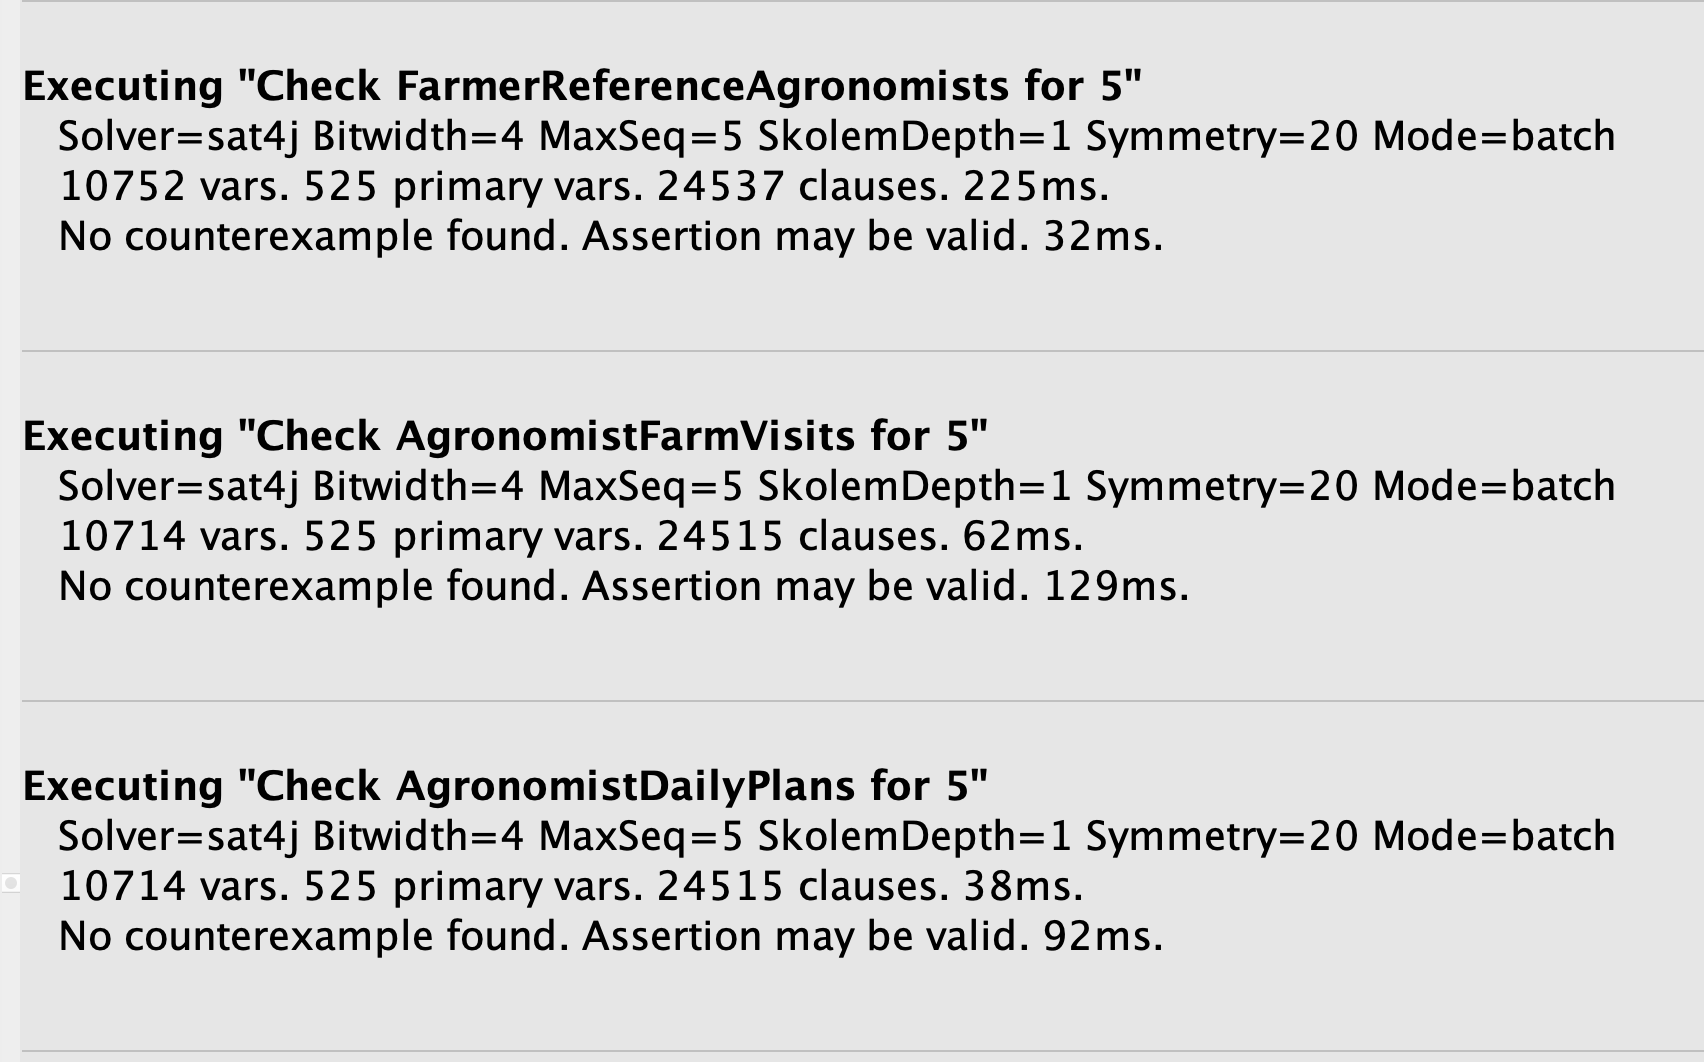
\includegraphics[scale=0.45]{alloy output/assertions.png}
    \caption{Output of the assertions.}
\end{sidewaysfigure}
\clearpage
\newpage
\clearpage
\begin{sidewaysfigure}
    \centering
    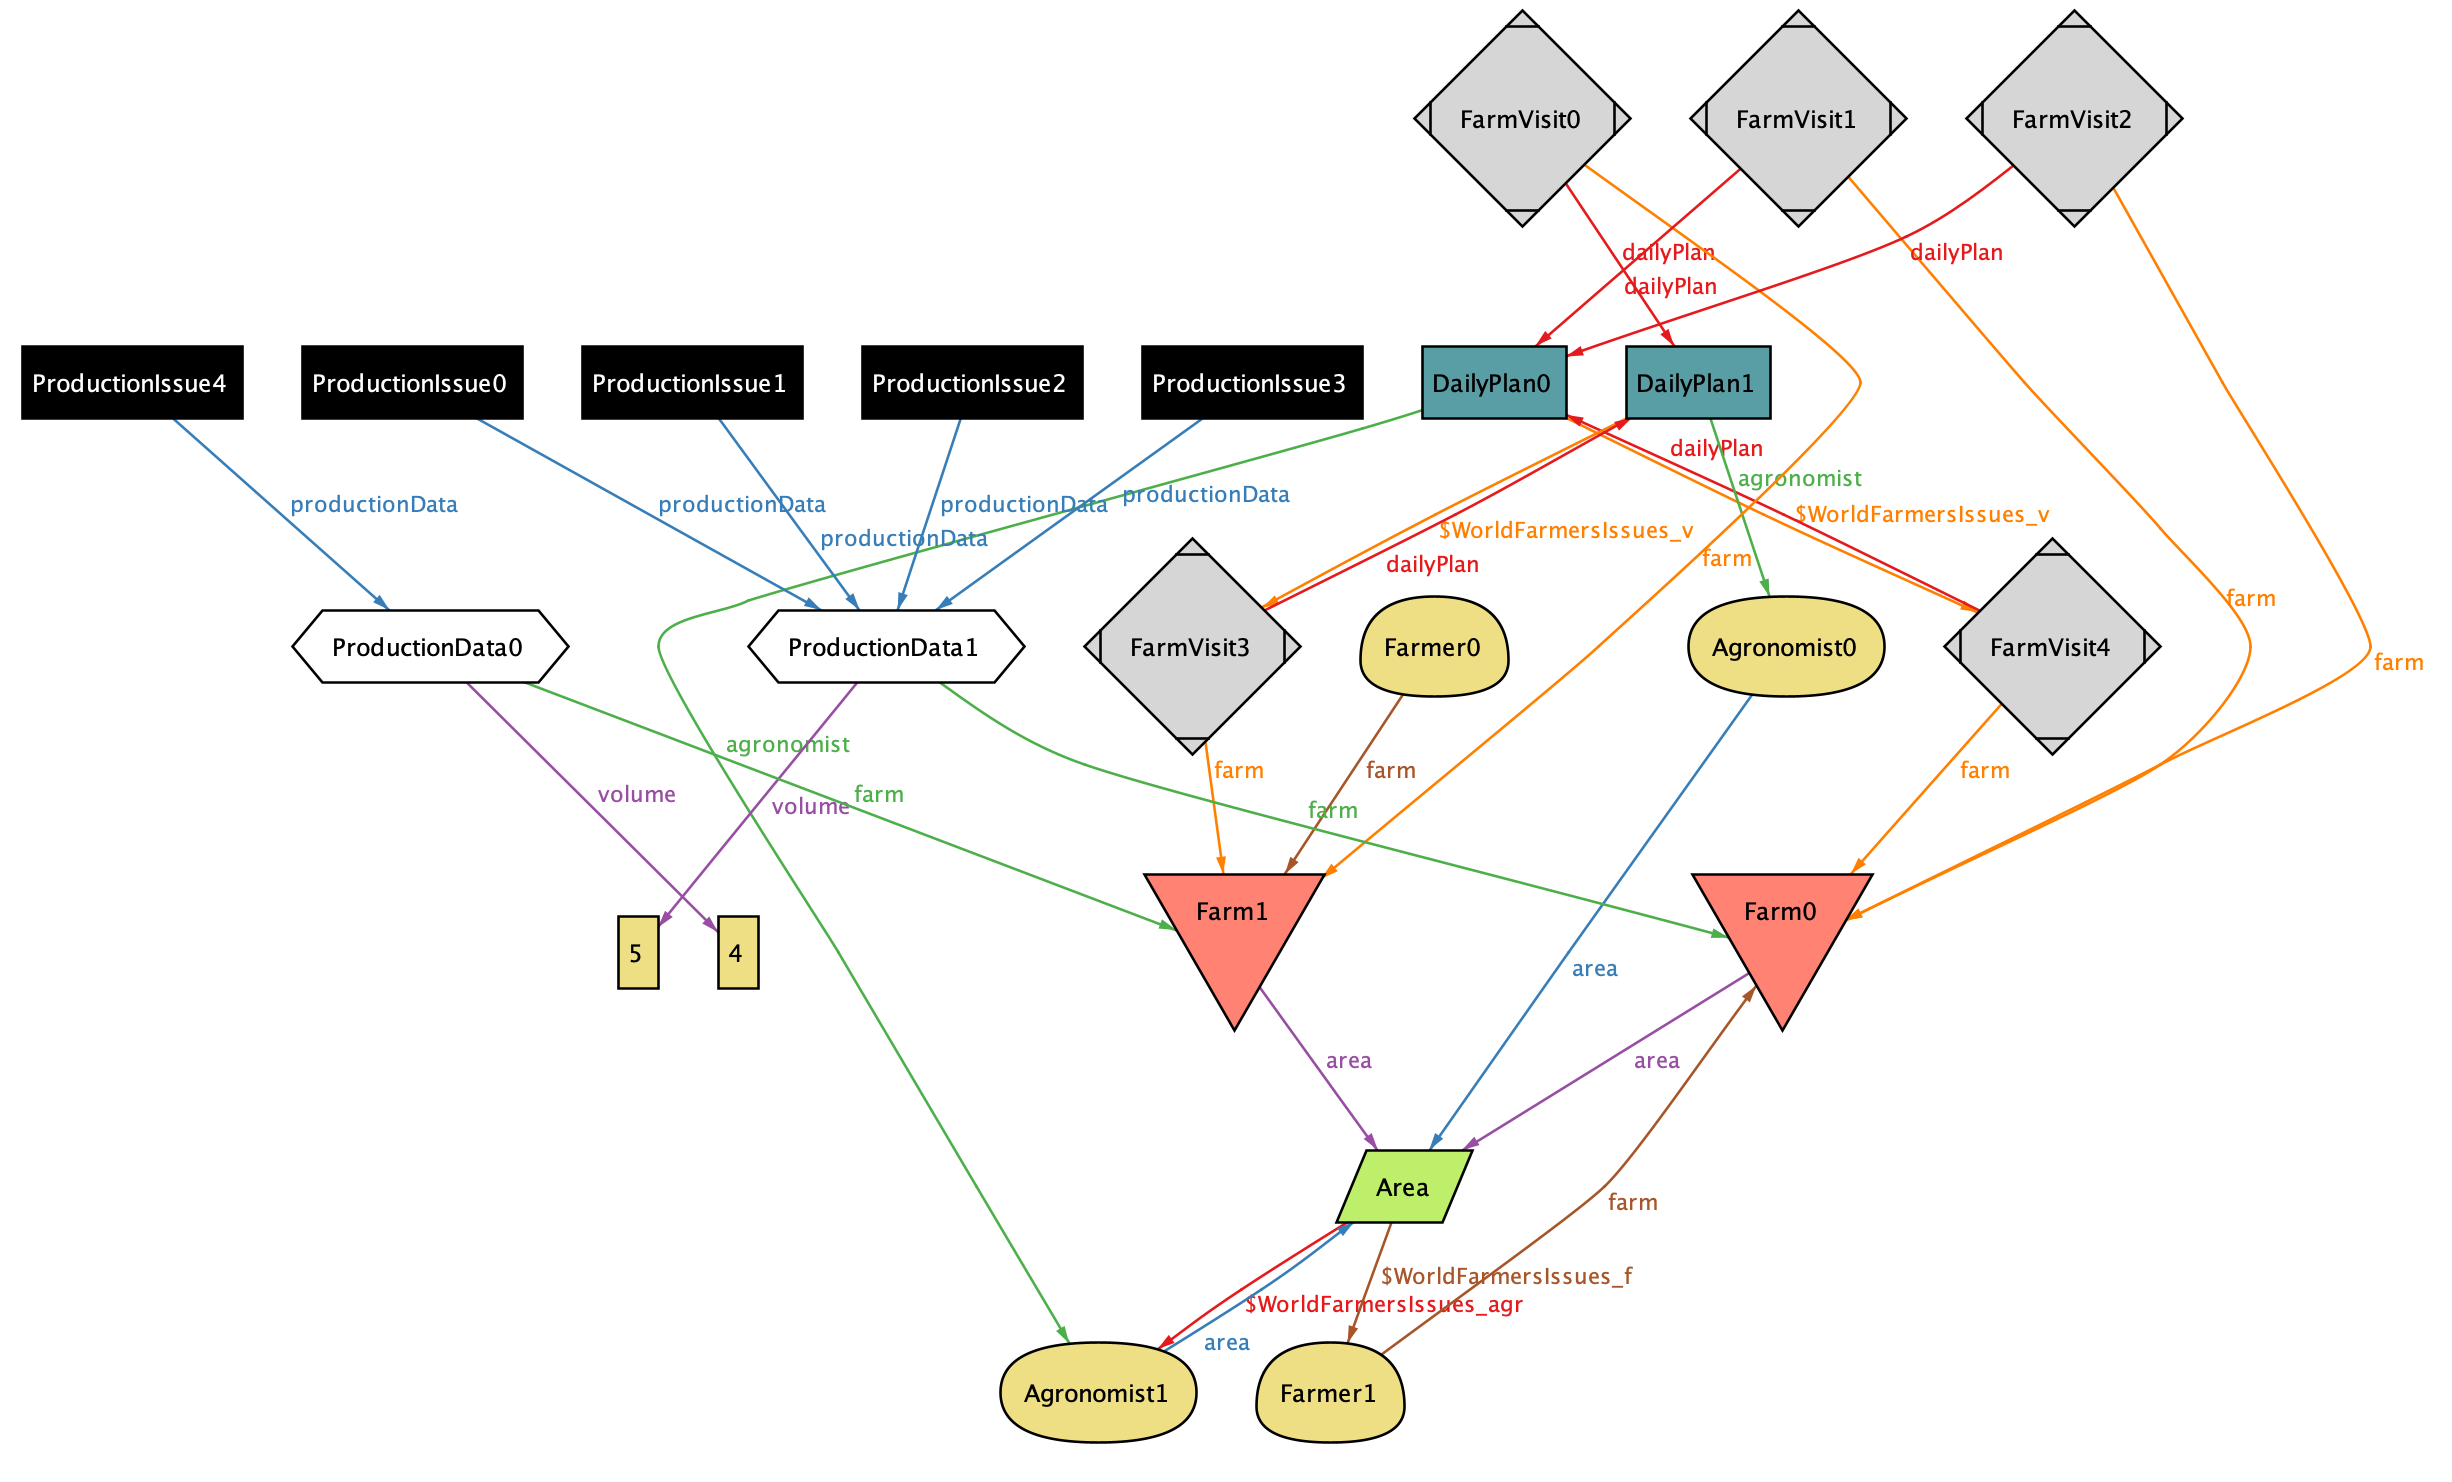
\includegraphics[scale=0.45]{alloy output/worldfarmersissues.png}
    \caption{Output of the "WorldFarmersIssues".}
\end{sidewaysfigure}
\clearpage
\newpage
\clearpage
\begin{sidewaysfigure}
    \centering
    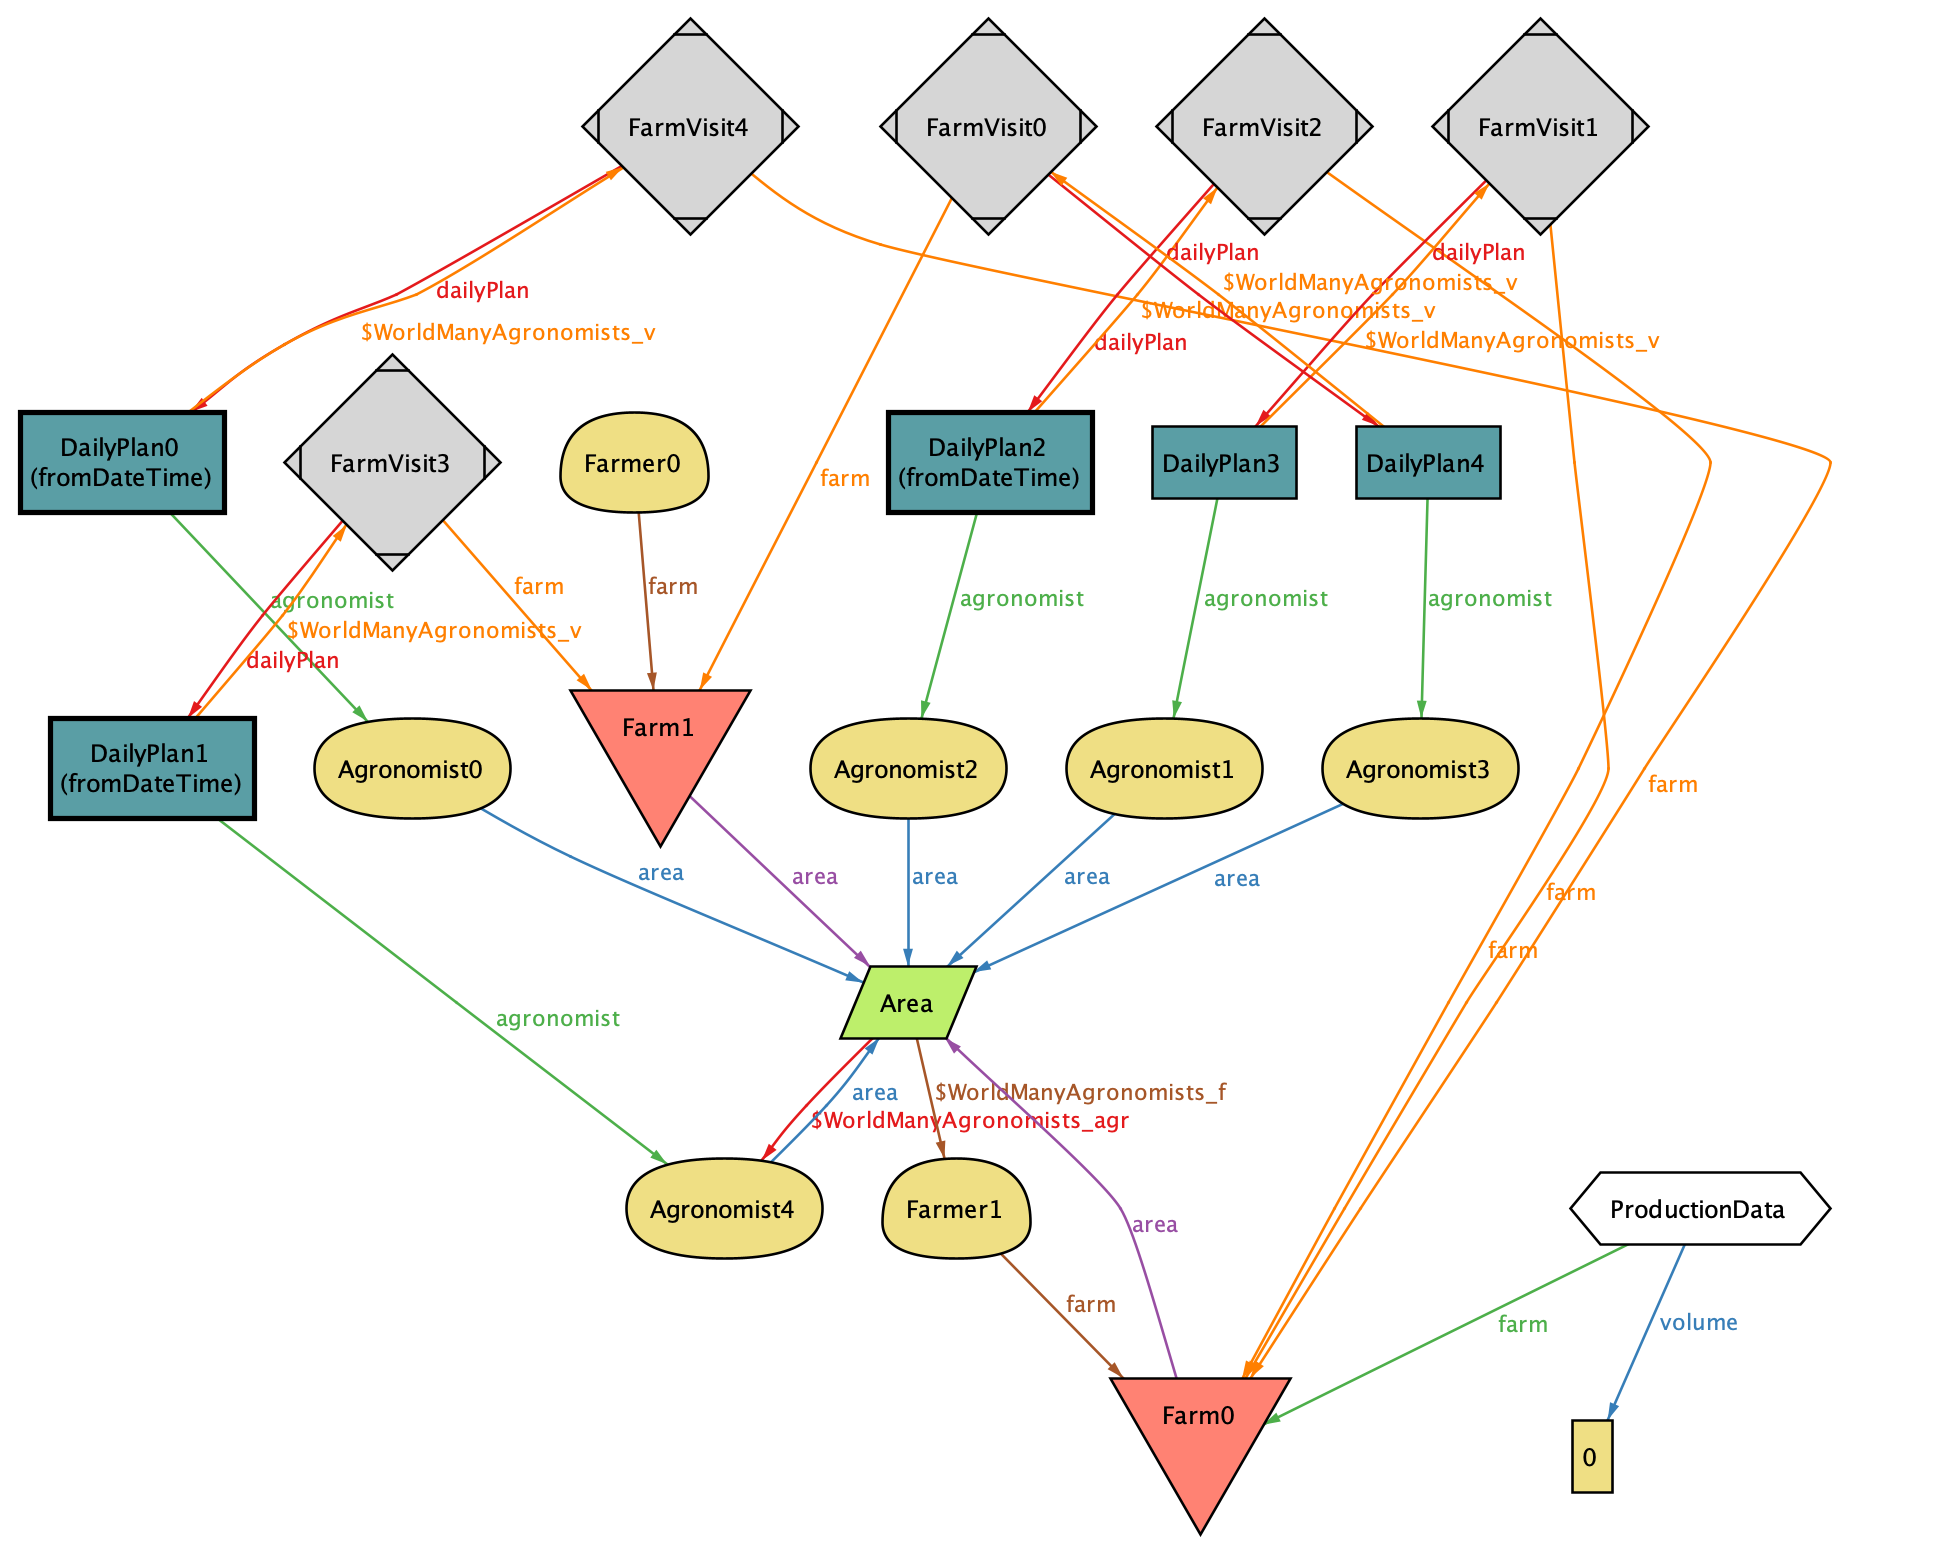
\includegraphics[scale=0.45]{alloy output/worldmanyagronomists.png}
    \caption{Output of the "WorldManyAgronomists".}
\end{sidewaysfigure}
\clearpage
\newpage
\clearpage
\begin{sidewaysfigure}
    \centering
    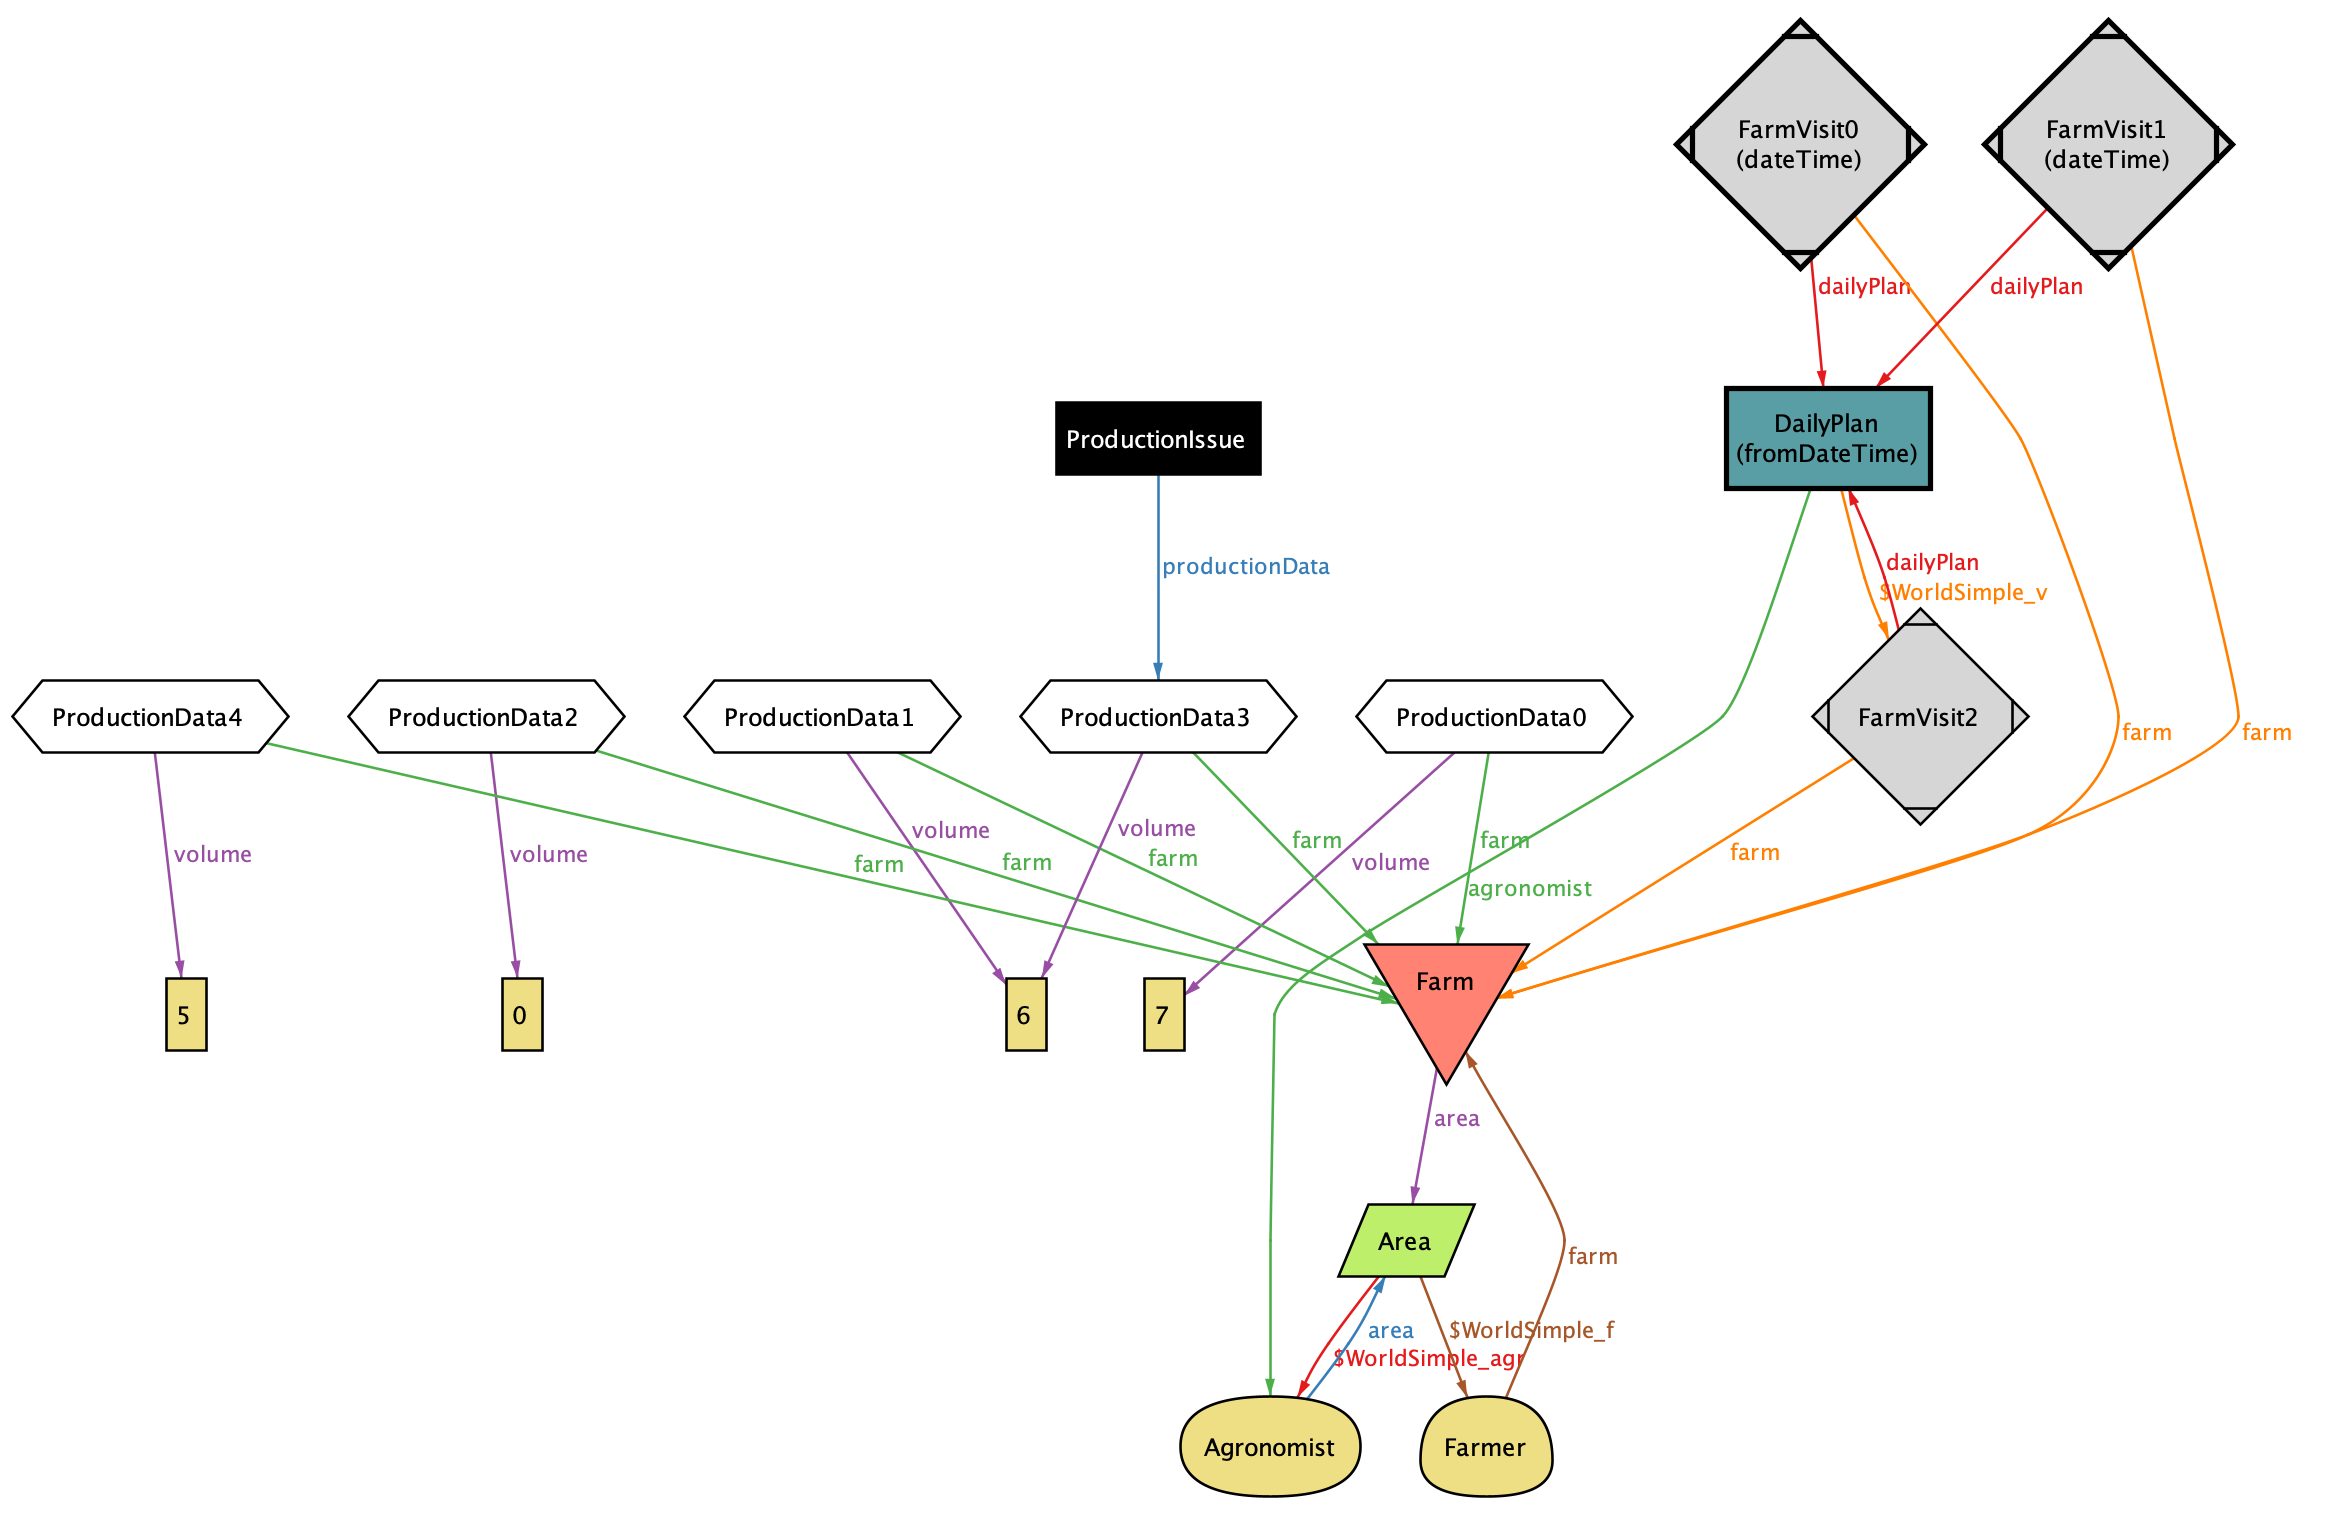
\includegraphics[scale=0.45]{alloy output/worldsimple.png}
    \caption{Output of the "WorldSimple".}
\end{sidewaysfigure}
\clearpage
\section{Effort spent}
\centering
\begin{longtable}{|m{5cm}|m{5cm}|}
\caption{The time Christian Grasso has spent on this document.}
 \label{christian effort spent}
 \hline
 \multicolumn{2}{|c|}{\cellcolor{white}\emph{Effort spent}} \\
  % do not write anything here
 \endfirsthead
 % do not write anything here
 \endhead
 % do not write anything here
 \endfoot
 % do not write anything here
 \endlastfoot
 \hline
 Organization\footnote{This entry features all the times the group gathered to decide what to do.} & 6h\\
 \hline
 Product perspective & 2.30h\\
 \hline
 Scenarios and use cases & 4h\\
 \hline
 WP SP G R D & 4h\\
 \hline
 Alloy & 9h\\
 \hline
 Review and Mockups & 4h\\
 \hline
 Final recap & 2h\\
 \hline
\end{longtable}

\centering
\begin{longtable}{|m{5cm}|m{5cm}|}
\caption{The time Filippo Lazzati has spent on this document.}
 \label{filippo effort spent}
 \hline
 \multicolumn{2}{|c|}{\cellcolor{white}\emph{Effort spent}} \\
  % do not write anything here
 \endfirsthead
 % do not write anything here
 \endhead
 % do not write anything here
 \endfoot
 % do not write anything here
 \endlastfoot
 \hline
 Organization\footnote{This entry features all the times the group gathered to decide what to do.} & 6h\\
 \hline
 Overall description & 4h\\
 \hline
 Scenarios and use cases & 12.30h\\
 \hline
 WP SP G R D & 9.30h\\
 \hline
 Alloy & 3h\\
 \hline
 External interfaces and performance requirements & 2.30\\
 \hline
 Review and Mockups & 3.30h\\
 \hline
  Final recap & 2h\\
 \hline
\end{longtable}

\centering
\begin{longtable}{|m{5cm}|m{5cm}|}
\caption{The time Chiara Magri has spent on this document.}
 \label{chiara effort spent}
 \hline
 \multicolumn{2}{|c|}{\cellcolor{white}\emph{Effort spent}} \\
  % do not write anything here
 \endfirsthead
 % do not write anything here
 \endhead
 % do not write anything here
 \endfoot
 % do not write anything here
 \endlastfoot
 \hline
 Organization\footnote{This entry features all the times the group gathered to decide what to do.} & 6h\\
 \hline
 Scenarios and use cases & 12.30h\\
 \hline
 Mapping R - UC & 5h\\
 \hline
 WP SP G R D & 14h\\
 \hline
 Alloy & 3h\\
 \hline
 Review & 1.30h\\
 \hline
  Final recap & 2h\\
 \hline
\end{longtable}
\newpage
\section{References}
\subsection{Used Tools}
\begin{itemize}
    \item \href{https://staruml.io/}{StarUML}: to draw UML diagrams;
    \item \href{https://app.diagrams.net/}{draw.io}: another tool to draw UML diagrams;
    \item \href{https://alloytools.org/}{Alloy}: to specify formally some requirements;
    \item \href{https://www.overleaf.com}{Overleaf}: Latex editor;
    \item \href{https://github.com/}{Github}: to share the files;
    \item \href{https://balsamiq.com/}{Balsamiq}: to design the wireframes.
\end{itemize}
\end{document}
